\documentclass[]{book}
\usepackage[]{epsf}
\usepackage{graphicx}
\usepackage{color}
%\usepackage{ams}
\usepackage{amssymb}
\usepackage{amsmath}
\usepackage{floatflt}
\usepackage[letterpaper]{geometry}
\usepackage{bezier}
\usepackage{kescust}
\usepackage{keslogic}
\usepackage{kescircuits}
\usepackage{circuitikz}
\usepackage{multirow}
\usepackage{rotating}
\usepackage{suffix}
\usepackage{wrapfig}
\usepackage[linesnumbered]{algorithm2e}%other options: ,lined,boxed,commentsnumbered

\newcommand{\NoSide}[1]{\multicolumn{1}{c}{#1}}
\newcommand{\RtSide}[1]{\multicolumn{1}{c|}{#1}}

\topmargin 0in \textheight 8.5in \textwidth 6.5in \evensidemargin
0in \oddsidemargin 0in


\newcommand{\sign}{\hbox{sgn}}

\ctikzset{bipoles/length=.6cm}
\newcommand\esymbol[1]{\begin{circuitikz}
\draw (0,0) to [#1] (1,0); \end{circuitikz}}
\WithSuffix\newcommand\esymbol*[1]{\begin{circuitikz}
\draw (1,0) to [#1] (0,0); \end{circuitikz}}


\input kvmacros %for karnaugh maps



\title{
{\Large Keith On...} \\
{\huge Hardware}
}
\author{
    K.E. Schubert \\
  \vspace{.1in} \\
  Founder \\
  Renaissance Research Labs \\
  \vspace{.1in} \\
  Professor \\
  Department of Electrical and Computer Engineering \\
  School of Engineering and Computer Science \\
  Baylor University 
}
\date{}

\makeindex

\begin{document}

\baselineskip=1.05\normalbaselineskip

\maketitle

\tableofcontents

%\listoffigures

%\listoftables

\pagenumbering{arabic}
\part{Electronics}
\chapter{Passive Components}


\section{Resistor}

\begin{eqnarray}
V &=& IR \\
P &=& VI \\
  &=& I^2R \\
  &=& \frac{V^2}{R}
\end{eqnarray}

DC: $R=\frac{l\cdot\rho}{A}$, where $l$ is the length in meters, $A$ is the cross sectional area in square meters and $\rho$ is the electric resistivity or specific electrical resistance in ohm-meters.  This assumes the current density is uniform.

\begin{picture}(200,200)(0,0)
\put(0,0){\Rvert{$222k\Omega$}}
\put(0,60){\Rhoriz{$222k\Omega$}}
%\put(70,79){\bezier{100}(0,0)(30,10)(40,40)}
\end{picture} 

\section{Capacitor}


\begin{eqnarray}
cV=q \label{cviq}
\end{eqnarray}
When I took my physics E\&M class my professor had an interesting way to remember equation~\ref{cviq}. One of his friends in college used a beer slogan, ``Canadian Velvet is the Queen of beers'', as a mnemonic.

\begin{picture}(200,200)(0,0)
\\put(70,0){\Cvert{$0.01\mu f$}}
\put(70,60){\Choriz{$0.01\mu f$}}
%\put(70,79){\bezier{100}(0,0)(30,10)(40,40)}
\end{picture} 

\section{Inductor}

Symbol: L

Unit: Henry (volt sec/Amp)

\begin{eqnarray}
\phi &=& LI
\end{eqnarray}
Note: $\phi$ is magnetic flux

\section{Memristence}

Memristors were first predicted in the 1970's due to symmetry, but were first made in 2007.  They have great potential to revolutionize memory.

\begin{eqnarray}
\phi &=& M(q)q
\end{eqnarray}
Thus, at some instant in time
\begin{eqnarray}
V(t) &=& M(q(t))I(t)
\end{eqnarray}
Note that $M$ is not a constant, and in fact it is non-linear with hysteresis.




\input{Kohw_basic_laws}
\chapter{Semiconductors}

This will be a brief introduction to physical electronics.  To properly study the field requires both quantum and statistical mechanics.  Perhaps one day I will write up a book on these topics and will then have the background material available to show more of the why.  For now I will attempt to give an understanding of the key concepts and an explanation of how to solve for key values.

\section{Energy Levels}

In electronics we are concerned about three basic types of materials: insulators, semiconductors, and conductors.  Their properties come from the energy gap between their valence\footnote{topmost filled band} (energy level of the valence band is denoted $E_v$) and conduction\footnote{band above the valence band} (energy level of the conduction band is denoted $E_c$) bands, and where the Fermi energy\footnote{A formal discussion is beyond the scope, so I will try to give a simple explanation.  In thermal equilibrium the Fermi energy is the chemical potential, i.e. the amount the energy of the system changes when particles are added or subtracted from it.  It is a crucial element in determining the probability a state contains an electron.  The Fermi energy can also be thought of as the critical energy of the Fermi-Dirac distribution (the energy at which the probability is $0.5$).  Note the Fermi energy is always greater than the energy of the highest filled band.} (denoted $E_f$) lies with respect to them.
\begin{description}
  \item[Conductors] have a small energy gap between the valence and conduction band and the Fermi energy is at or above the level of the conduction band.  Charge carriers are readily available to carry current.  This is how they conduct.
  \item[Semiconductors] have a small to mid sized gap and the Fermi energy lies in this gap.  Charge carriers are not readily available, but can be made to be available by other factors (temperature, electric field, photons, donors/acceptors, etc.).  This ability to conduct or insulate is the source of the name.  We break down semiconductors into different categories: intrinsic and extrinsic.  Extrinsic is then broken down into p or n type.
  \item[Insulators] have a large energy gap between the valence and conduction band and the Fermi energy is between them, though not close to the conduction band.  This means charge carriers are very unlikely available to move and thus carry current.  This is how they insulate.
\end{description}
Quantum theory tells us that the electrons around an atom are in shells that have quantized energy values.  Further, due to the Pauli Exclusion Principle, no two electrons can have the same quantum numbers (n, l, m, s), which also applies in systems of multiple atoms.  As atoms come closer together the shells split so the quantum numbers are unique between them.


%To explain where these energies come from we need to do a brief review of some results from quantum theory.  The total energy of an electron bound to a hydrogen nucleus is given by
%\begin{eqnarray}
%E(n) &=& \frac{-m_eq^4}{8\pi^2\epsilon_0^2\hbar^2n^2}\\
%     &=& \frac{-m_eq^4}{2\epsilon_0^2h^2n^2}
%\end{eqnarray}
%where
%\begin{description}
%  \item[$n$] n is the principle quantum number and takes the values of $\{1, 2, \ldots\}$.
%  \item[$m_e$] mass of an electron ($9.11\times 10^{-31}$ [kg]).
%  \item[$q$] charge of an electron ($1.6\times 10^{-19}$ [C]).
%  \item[$\epsilon_0$] permittivity of free space ($8.85\times 10^{-12}$ [F/m]).
%  \item[$\hbar$] modified Planck's constant ($1.054\times 10^{-34}$ [J-s]), which is just Planck's constant divided by $2\pi$.
%  \item[$h$] Planck's constant ($6.625\times 10^{-34}$ [J-s]).
%\end{description}




\section{Intrinsic Semiconductors}

Intrinsic semiconductors are materials that semiconduct in and of themselves.  They come in two varieties, elemental (Si, Ge) and compound (GaAs, InP, etc.), which simply tells you if the material is an element or a compound (made of several elements).  Elemental semiconductors come from column IVa of the periodic table, see Table~\ref{t-PeriodicTable}, as they have half their outer s and p sub-shells filled.  Compound intrinsic semiconductors are compounds that behave like elemental intrinsic semiconductors, as they are formed by bonding elements on either side of column IVa.  I will mostly discuss elemental, though the principles are the same for compound intrinsic semiconductors.

\begin{table}
\caption{Semiconductors in the Periodic Table and Intrinsic Semiconductor Properties}\label{t-PeriodicTable}\label{T:IntSemi}
\begin{tabular}{cc}
\begin{tabular}{|c|c|c|c|c|c|}
\NoSide{IB}    & \NoSide{IIB}   & \NoSide{IIIA}  & \NoSide{IVA}   & \NoSide{VA}    & \NoSide{VIA}   \\
\cline{3-6}
\NoSide{}      & \RtSide{}      & 5              & 6              & 7              & 8              \\
\NoSide{}      & \RtSide{}      & B              & C              & N              & O              \\
\cline{3-6}
\NoSide{}      & \RtSide{}      & 13             & 14             & 15             & 16             \\
\NoSide{}      & \RtSide{}      & Al             & Si             & P              & S              \\
\hline
29             & 30             & 31             & 32             & 33             & 34             \\
CU             & Zn             & Ga             & Ge             & As             & Se             \\
\hline
47             & 48             & 49             & 50             & 51             & 52             \\
Ag             & Cd             & In             & Sn             & Sb             & Te             \\
\hline
79             & 80             & 81             & 82             & 83             & 84             \\
Au             & Hg             & Tl             & Pb             & Bi             & Po             \\
\hline
\end{tabular}
%\end{table}
%\begin{table}
%\caption{Properties of intrinsic semiconductors.}\label{T:IntSemi}
&
\begin{tabular}{lccc}
Material          & Symbol & $E_g$[$eV$] & B[$cm^{-3}K^{-3/2}$]\\\hline
%Gallium Nitride   & GaN    & 3.5         & \\
%Gallium Phosphide & GaP    & 2.26        &                      \\
Gallium Arsenide  & GaAs   & 1.42        & $2.10\times 10^{14}$ \\
Germanium         & Ge     & 0.66        & $1.66\times 10^{15}$ \\
Silicon           & Si     & 1.12        & $5.23\times 10^{15}$ \\
\end{tabular}
\\ \end{tabular}
\end{table}

%Silicon, Si - the most common semiconductor, atomic number 14, energy gap Eg = 1.12 eV - indirect bandgap; crystal structure - diamond, lattice constant 0.543 nm, atomic concentration 5x1022 atoms/cm-3, index of refraction 3.42, density 2.33 g/cm3, dielectric constant 11.7, intrinsic carrier concentration 1.02 x 1010 cm-3, mobility of electrons and holes at 300 K: 1450 and 500 cm2/V-s, thermal conductivity 1.31 W/cm-oC, thermal expansion coefficient 2.6 x 10-6 1/oC, melting point 1414 oC; excellent mechanical properties (MEMS applications); single crystal Si can be processed into wafers up to 300 mm in diameter.

%Ge, C, Sb.


%Gallium Arsenide, GaAs - After silicon second the most common semiconductor, energy gap Eg = 1.43 eV, direct bandgap; crystal structure - zinc blend, lattice constant 5.65 Ang., index of refraction 3.3, density 5.32 g/cm3, dielectric constant 12.9, intrinsic carrier concentration 2.1 x 106 cm-3, mobility of electrons and holes at 300 K - 8500 and 400 cm2/V-s, thermal conductivity 0.46 W/cm-oC, thermal expansion coefficient 6.86 x 10-6 oC-1; thermally unstable above 600 oC due to As evaporation; does not form sufficient quality native oxide; mechanically fragile; due to direct bandgap commonly used to fabricate light emitting devices; due to higher electron and hole mobilities, also foundation of the variety of high-speed electronic devices; bandgap can be readily engineered by forming ternary compounds based on GaAs, e.g. AlGaAs.

%Gallium Nitride, GaN - wide bandgap III-V semiconductor with direct bandgap 3.5 eV wide; among very few semiconductors capable of generating blue radiation, GaN is used for blue LEDs and lasers; intrinsically n-type semiconductor but can be doped p-type; GaN is formed as an epitaxial layer; Lattice mismatch remains a problem, creating a high defect density. Incorporation of Indium (InxGa1-xN) allows control of emission from green to violet (high and low In content respectively). GaN can also be used in UV detectors that do not respond to visible light. GaN has a Wurtzite(W) or Zinc Blend(ZB) crystal structure. Lattice constant [A] 3.189(W) 5.186(ZB); Density[g/cm3] 6.15(W) 6.15(ZB); Atomic concentration [cm-3] 8.9 x 1022(W) 8.9 x 1022(ZB); Melting point [oC] 2,500(W) 2,500(ZB); Thermal conduct.[W/cm oC] 1.3(W) 1.3(W); Thermal expansion coefficient[oC-1] ~1x10-6; Dielectric constant (static) 8.9(W) 9.7(ZB); Refractive index 2.4(W) 2.3(ZB);

%GaP - Crystal structure zinc blend; Lattice constant [A] 5.45; Density [g/cm3] 4.14; Atomic concentration [cm-3] 4.94 x 1022; Melting point [oC] 1457; Thermal conductivity [W/cm oC] 1.1; Thermal expansion coefficient[1/oC] 4.65x10-6; Dielectric constant 11.1; Refractive index 3.02; Energy gap [eV] 2.26; Type of energy gap: direct; Electron mobility [cm2/V sec] 250; Hole mobility [cm2/V sec] 150;

% CdSe, CdTe, CdHgTe, ZnS

%Silicon carbide, SiC - semiconductor featuring energy gap Eg = 2.9 -3.05 eV (wide bandgap semiconductor), indirect bandgap; SiC can be obtained in several polytypes- most common hexagonal in the form of either 4H or 6H polytypes; parameters vary depending on polytype; Intrinsically n-doped; p-type doping and n-type conductivity control can be obtained by doping with aluminum and nitrogen respectively. SiC features higher than Si and GaAs electron saturation velocity; excellent semiconductor but difficult and expensive to fabricate single-crystal wafers; excellent for high power, high temperature applications; SiC is closely lattice matched to GaN, has a thermal expansion coefficient close to GaN, and is available in both conductive and semi-insulating substrates. Thus it is often used as a substrate for GaN epitaxial layers. SiC wafers 75 mm in diameter are available commercially.
%Crystal Structure 3C-SiC (cubic) 6H-SiC (hexagonal)
%Lattice constant [A] 4.36 3.08
%Thermal conductivity [W/cm oC] 5
%Melting point sublimes > 2,100 oC
%Dielectric constant 9.7
%Energy gap [eV] 2.3 3.03
%Electron Drift Mobility [cm2/V sec] 800 400
%Hole Drift Mobility [cm2/V sec] 40 100



%Equations used to calculate Direct Energy Gap
%AlxIn1-xP 1.34 + 2.23x
%AlxGa1-xAs 1.424 + 1.247 (x<0.45)
%1.424 + 1.087x + 0.438x2
%AlxIn1-xAs 0.36 + 2.35x + 0.24x2
%AlxGa1-xSb 0.73 + 1.10x + 0.47x2
%AlxIn1-xSb 0.172 + 1.621x + 0.43x2
%GaxIn1-xP 1.34 + 0.511x + 0.6043x2
%(0.49
%GaxIn1-xAs 0.356 + 0.7x + 0.4x2
%GaxIn1-xSb 0.172 + 0.165x + 0.413x2
%GaPxAs1-x 1.424 + 1.172x + 0.186x2
%GaAsxSb1-x 0.73 - 0.5x + 1.2x2
%InPxAs1-x 0.356 + 0.675x + 0.32x2
%InAsxSb1-x 0.18 - 0.41x + 0.58x2
%Source: Swaminathan, V; Macrander, A. T.; Materials Aspects of GaAs and InP based Structures. 1991.


\begin{wrapfigure}{r}{0.4\textwidth}
%\vspace*{-.45in}
\begin{center}
\caption{Silicon crystal structure}
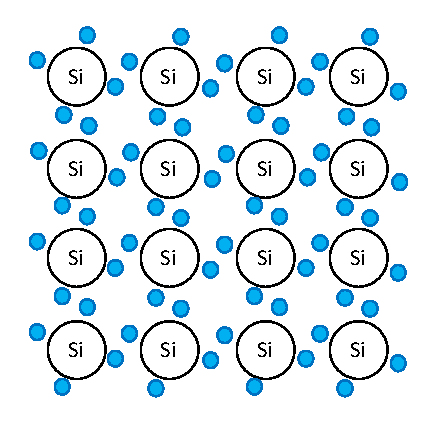
\includegraphics[width=0.35\textwidth]{semiconductors_pure}\label{f-semiconductor-pure}
\end{center}
\end{wrapfigure}

These are (and must be) pure materials, as even a small amount of impurities will cause them not to work.  Most modern semiconductors are extrinsic\footnote{This is due to the excessive cost and difficulty of making a pure or nearly pure material.}, so I will just give a brief overview.  At room temperature, Fermi-Dirac statistics shows the gap between valence and conduction band must be on the order of 1 electron volt or less.  Several materials meet this requirement, such as gallium arsenide (GaAs, 1.42 eV), Silicon (Si, 1.12 eV), and Germanium (Ge, 0.66 eV).  The electrons promoted to the conduction band leave behind holes in the valence band, and current is carried by both the flow of electrons in the conduction band and holes in the valence band.  The flow of the electron-hole pairs (in opposite directions) is the mechanism of current.  Essentially the electron-hole movement is the same for extrinsic semiconductors also, but for extrinsic semiconductors these need not be equal (and are not).

The number of electrons available in the conduction band is  given by
\begin{eqnarray}
n_e &=& 2\left(\frac{2\pi m^*_nkT}{h^2}\right)^{\frac{3}{2}}e^{\left(\frac{-(E_c-E_f)}{2kT}\right)}\\
&=&BT^{\frac{3}{2}}e^{\left(\frac{-(E_c-E_f)}{2kT}\right)}
\end{eqnarray}



Since the number of electrons in the conduction band and the number of holes in the valence band are equal in an intrinsic semiconductor, we will just consider the density of the intrinsic carriers (either electron or hole), $n_i$.
\begin{eqnarray}
n_i &=& BT^{\frac{3}{2}}e^{\left(\frac{-E_g}{2kT}\right)}
\end{eqnarray}
The temperature in Kelvin is $T$.  The values of $B$ and $E_g$ are dependent on the material, and are provided for our top three intrinsic materials in Table~\ref{T:IntSemi}.The Boltzmann constant, $k$, is $86\times 10^{-6}$[$eV/K$].

\begin{example}
What is the carrier density of Germanium at room temperature?

Answer:

Room temperature is not a well defined term, meaning it is not a set temperature.  Roughly it could vary from $65^\circ$F to $85^\circ$F, or in kelvin, from 291K to 303K.  For ease of calculation, we will choose 300K to be room temperature.
\begin{eqnarray}
n_i
&=& BT^{\frac{3}{2}}e^{\left(\frac{-E_g}{2kT}\right)} \\
&=& 1.66\times 10^{15}\cdot 300^{\frac{3}{2}}e^{\left(\frac{-0.66}{2\cdot 86\times 10^{-6} \cdot 300}\right)}\\
&\approx & 2.40\times 10^{13} [cm^{-3}]
\end{eqnarray}
\end{example}

To make life easier in calculating this, I usually use a small SciLab program, see Code~\ref{code:intrinsicCarriers}.

\SciLab{SciLab code to calculate intrinsic carrier density.}{code:intrinsicCarriers}{IntrinsicCarriers.sce}

\section{Extrinsic Semiconductors}

Extrinsic semiconductors are made by adding an impurity into the crystallin structure that is chosen to provide an extra electron above the valence band (a donor or n type), or to provide a deficiency of electrons (an acceptor or p type).  Since the charge carriers (electrons and holes) are no longer balanced, we need to be able to calculate how many of them there are.  A basic relationship is
\begin{eqnarray}
n_e n_h &=& n_i^2 \label{eq:extrinsiccarrierdensity}
\end{eqnarray}
where $n_e$ is the thermal equilibrium concentration of free electrons, $n_h$ is the thermal equilibrium concentration of holes, and $n_i$ is the intrinsic carrier density.  Provided the concentration of the dopant is greater than the intrinsic carrier density, we can approximate the number of carriers of the type provided by the dopant by the concentration of the dopant.  We will denote the dopant concentration by $N_n$ for n type materials and $N_p$ for p type materials.

%A p-type wafer is usually doped with Boron, although Gallium can also be used (rare). P+ wafers are heavily doped and typically have resistances of <1 Ohm/cm2. P+ wafers are often used for Epi substrates. P- wafers are lightly doped with typical resistances of >1 Ohm/cm2. The most common crystal orientations for P-type wafers are {100} and {111}.

%N-type wafers are doped with Phosphorus, Antimony, or Arsenic. N+ wafers are heavily doped with resistances <1 Ohm/cm2. N- wafers are lightly doped with resistances >1 Ohm/cm2.

%Resistivity is very important to good electronic devices and for growing uniform thermal oxides. High resistivity silicon can only be produced using the Float Zone (FZ) crystal growth method, which does not use a crucible during crystal growth. The Czochralski (CZ) method uses a quartz crucible during crystal growth, and oxygen from the crucible unintentionally dopes the material. The oxygen dopant behaves as an n-type impurity and impedes high resistivity. Low resistivity n-type material is achieved using Arsenic doping.

%Wafer flats in relation to doping



\subsection{P Type Semiconductors}

\begin{figure}
\begin{center}
\caption{P Type Silicon crystal structure}\label{f-semiconductor-p}
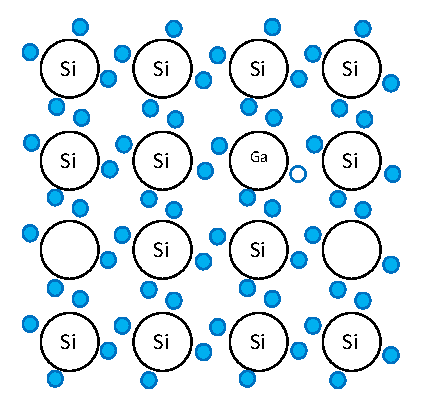
\includegraphics{semiconductors_p}
\end{center}
\end{figure}
If an element like gallium or boron is doped, which has only 3 electrons in its outer shell of up to 8, into the crystallin structure of say silicon, which has 4 electrons in its outer shell of 8, a gap in the bonding is formed, see Figure~\ref{f-semiconductor-p}.  The outer shell of the gallium and the bonded silicon is just one shy of completing and thus it is already free to conduct a hole by stealing an electron from a neighbor.  In terms of energy bands, the energy of this ``hole'' (usually denoted $E_a$) is very close to (but above) the energy of the valence band.  The Fermi energy is thus close to the valence band, which means there will not be lots of free electrons, so the only free carriers are these holes\footnote{In truth the hole is the spot where the electron is missing (and thus not an actual thing), but since this means that the atom that is missing it is ionized (positive in the case of a lack of an electron), it appears that a positive charge is flowing.  This is governed by statistical mechanics and so it is not possible to track the actual electron.  Like it or not, holes are a reasonable description of how the charge is carried.}.

\subsection{N Type Semiconductors}
\begin{figure}
\begin{center}
\caption{N Type Silicon crystal structure}\label{f-semiconductor-n}
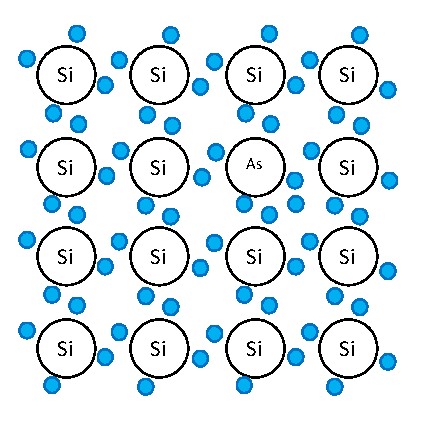
\includegraphics{semiconductors_n}
\end{center}
\end{figure}




\chapter{Diodes}

Up till now we have considered individual semiconductors, now we want to consider what happens when we put two next to each other.  By placing a p region next to an n region, holes start diffusing from the p region to the n region, and electrons start diffusing from the n region to the p region.  This does several things.  
\begin{itemize}
\item First, it locks up the charge carriers, so that there are not any available to carry current.  For this reason it is called the depletion region.  
\item Second, it causes a charge differential across the boundary, which is called the potential barrier, $V_{bi}$.  The potential barrier resists the further diffusion of charge carriers, because the depletion region in the n material is slightly positive, and the depletion region in the p region is slightly negative, resulting in an induced E-field from n to p.  The potential barrier is given by
    \begin{eqnarray}
    V_{bi} &=& \frac{kT}{e^-}\ln{\left(\frac{N_nN_p}{n_i^2}\right)},
    \end{eqnarray}
    where, $e^-$ is the electron charge\footnote{I am putting a minus sign in the exponent to distinguish the electron charge from the natural logarithm base.  Thus I will put a plus in the exponent if I want to speak of the charge of a proton.  The value of $e^-=1.602176487�10^{-19}$ [coulombs], which can also be calculated by $e^-=\frac{F}{N_A}$, where $F$ is Faraday's constant ($9.64853399x10^4$ [C/mol]) and $N_A$ is Avogadro's Number ($6.02213667x10^{23}$ [1/mol]).}.  We often lump $\frac{kT}{e^-}$ into a term called the thermal voltage, $V_T$, which is approximately $V_T\approx 0.026$ [V] at $T=300$ [K].
\item Third, the charge differential acts like a capacitor (it is storing charge).  The nominal (or zero applied voltage) junction capacitance (or depletion layer capacitance), is given by, $C_{j0}$ and is usually around a pico Farad (pF).
\end{itemize} 

\section{Reverse Bias}

If we apply a voltage, such that the positive terminal is connected to the n material, and the negative terminal to the p material, the applied electric field, $E_A$, is in the same direction as the electric field of the potential barrier.  This causes the depletion region to grow, because the free electrons in the n material are drawn to the positive terminal and the free holes in the p material are drawn to the negative terminal.  The larger depletion region prevents charge from flowing so the diode is off.  The reverse bias also effects the junction capacitance.
\begin{eqnarray}
C_j &=& C_{j0}\left(1+\frac{V_R}{V_bi}\right)^{-0.5}
\end{eqnarray}
with $V_R$ the reverse bias voltage.  Note the larger the larger the applied voltage the smaller the capacitance, which is due to the increased width of the depletion region (wider the region the lower the capacitance). 
\chapter{Binary Junction Transistors}

\begin{tabular}{l|ccc}
Characteristic   & Common Base & Common Emitter & Common Collector \\\hline
Input impedance  & Low         & Medium         & High \\
Output impedance & Very High   & High           & Low \\
Phase Angle      & $0^\circ$   & $180^\circ$    & $0^\circ$ \\
Voltage Gain     & High        & Medium         & Low \\
Current Gain     & Low         & Medium         & High \\
Power Gain       & Low         & Very High      & Medium \\
\end{tabular}
\chapter{Field Effect Transistors}

\section{Ideal Behavior}

A Field Effect Transistor (FET) is in one sense essentially a capacitor, and thus it is governed by
\begin{eqnarray}
CV &=& Q\\
C_{gb}(V_{gc}-V_t) &=& Q_{channel}
\end{eqnarray}
where,
\begin{itemize}
\item $C_{gb}$ is the capacitance between the gate and the body, this is often just called the gate capacitance.
\item $V_{gc}$ is the Voltage between the gate and the channel.  Note that $V_c=V_{ds}/2$, so $V_{gc}=V_gs-V_{ds}/2$.
\item $V_t$ is the threshold voltage, i.e. the minimum voltage to cause an inversion layer to form.
\item $Q_{channel}$ is the charge carries available in the channel to conduct.
\end{itemize}
The more charge carriers, $Q_{channel}$, the easier the current will flow, so calculating this is an essential step to quantitatively analyzing a FET.  First we need to find out what our capacitance, $C_{gb}$ is, this is done by
\begin{eqnarray}
C_{gb} &=& \varepsilon_{ox}\frac{WL}{t_{ox}} \\
&=& 3.9\varepsilon_0\frac{WL}{t_{ox}}
\end{eqnarray}
\begin{itemize}
\item $\varepsilon_{ox}$ is the permittivity\footnote{Permittivity is the resistance to forming an electric field.} of the insulating oxide layer.  Note: the 3.9 is the relative permittivity of silicon dioxide compared the the permittivity of free space.  Relative permittivity is denoted $\varepsilon_r$, and varies by material, frequency, temperature, and sometimes even direction.  We will treat it as a constant, which is ok for our operating situation.
\item $\varepsilon_0$ is the permittivity of free space ($8.85 \times 10^{-14}$ [F/cm]).
\item $W$ is the width of the gate (along source and drain).
\item $L$ is the length under the gate (between source and drain).
\end{itemize}
Now we want to get the current flowing in the channel, but that means we need to know how fast they are moving.  In a semiconductor the velocity of the charge carrier, $v_c$, is given by
\begin{eqnarray}
v_c &=& \mu_cE\\
&=&\mu_c\frac{V_{ds}}{L}
\end{eqnarray}
where $\mu_c$ is the mobility of the charge carrier.  The length of the channel divided by the velocity of the carriers, gives us the time for a charge to cross the channel, $T_{channel}$.  The total charge in the channel divided by this time is then the current.
\begin{eqnarray}
i_{ds} &=& \frac{Q_{channel}}{T_{channel}}\\
 &=& \frac{C_{gb}(V_{gc}-V_t)}{\frac{L}{v_c}}\\
 &=& \frac{3.9\varepsilon_0\frac{WL}{t_{ox}}(V_{gc}-V_t)}{\frac{L}{\mu_c\frac{V_{ds}}{L}}}\\
 &=& 3.9\varepsilon_0\frac{W}{t_{ox}}(V_{gs}-V_t)\mu_c\frac{V_{ds}}{L}\\
 &=& \frac{3.9\varepsilon_0}{t_{ox}}\mu_c\frac{W}{L}(V_{gc}-V_t)V_{ds}\\
 &=& \frac{3.9\varepsilon_0}{t_{ox}}\mu_c\frac{W}{L}(V_{gs}-V_t-V_{ds}/2)V_{ds}
\end{eqnarray}


\section{Amplification}

\begin{eqnarray}
i_{DS} &=& \frac{k}{2}(V_{GS}-V_T)^2
\end{eqnarray}
if $V_{DS} \geq V_{GS}-V_T\geq 0$. 
\chapter{Logic Families}

There are a great many logic families in use today.  Probably the most famous is the TTL family, though it has largely been replaced by CMOS families.  Even so, there are reasons for using different families (power, current, voltage, static, noise rejection, bus design, etc.).  In the following sections we will examine some of the more well known families, their advantages, and how to interface them.


\section{Diode Logic}
Diode Logic (DL) uses diodes and resistors to implement logic gates.  DL is a simple but old technology not used in integrated circuits.  They are helpful to understand, as they are similar in some ways to later families.  DL only has \textbf{and} and \textbf{or} gates.

\begin{figure}
\begin{center}
\caption{Diode Logic  (a) \textbf{Or} Gate\label{f:DL_or} and (b) \textbf{And} Gate.}\label{f:DL_and}
\begin{tabular}{cc}
(a) & (b) \\
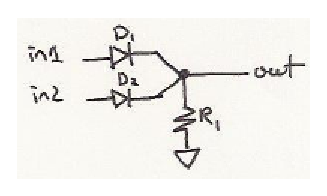
\includegraphics{images/DLor.eps}&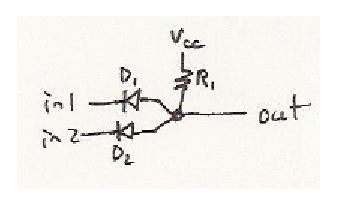
\includegraphics{images/DLand.eps}\\
\end{tabular}
\end{center}
\end{figure}
Consider the circuit in Figure~\ref{f:DL_or}.  If either $in_1$ or $in_2$ is high, the corresponding diodes ($D_1$ or $D_2$ respectively) turns on, making the output high.  Since the output will be about 0.6v less than the input you can't put too many of these in series before the logic level drops below useful levels.  If both inputs are off then both diodes don't conduct and the resistor to ground ($R_1$) pulls the output down to a low output (hence the name pull down resistor).  The circuit is thus an \textbf{or} gate.

Now consider the circuit in Figure~\ref{f:DL_and}.  If either $in_1$ or $in_2$ is low, the corresponding diodes ($D_1$ or $D_2$ respectively) turns on, making the output low, though it will be about 0.6v higher than the inputs so just like with the \textbf{or} gate, you can't do too many of these in series.  If by inputs are high, then both diodes are off and the output is isolated from the input.  The resistor to $V_{cc}$ pulls the output up (hence the name, pull up resistor).  The gate is thus an \textbf{and} gate.


\section{Resistor Transistor Logic}
Resistor Transistor Logic, (RTL) replaces the diodes of DL with transistors, which allowed for negation.  This is thus the first full logic family.


\section{Diode Transistor Logic}


\begin{figure}
\begin{center}
\caption{Diode Transistor Logic \textbf{Nand} Gate.}\label{f:DTL_nand}
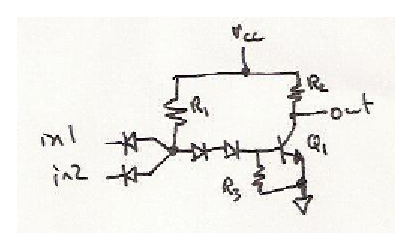
\includegraphics{images/DTLnand.eps}
\end{center}
\end{figure}

\section{Transistor Transistor Logic}
Transistor transistor logic (TTL) is arguably the most famous logic family.  It has been used for around 40 years, and can still be purchased today.  It is reasonably fast, has good noise rejection, and has good protection from static.  A large number of interfaces are TTL compatible, so even when the components are not used, its design implications are still felt.  The venerable 7400 and 5400 (milspec\footnote{Milspec means it is built to military specification, which would be enough to be noteworthy, but milspec parts are useful in hazardous environments, such as space, marine (water and saline), industrial fabrication environments, extreme temperature ranges, etc.}) series are the most famous TTL components, and they have been used widely in engineering labs since I was in school way back when...  If you want to see what components were in the series, see Appendix~\ref{c:7400}.



\begin{figure}
\begin{center}
\caption{Transistor Transistor Logic \textbf{Nand} Gate.}\label{f:TTL_nand}
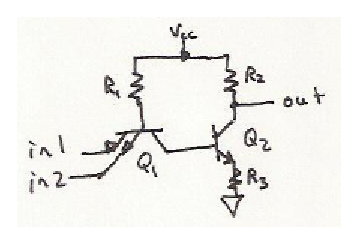
\includegraphics{images/TTLnand.eps}
\end{center}
\end{figure}

\subsection{Open Collector Outputs}
If you noticed in earlier logic families, typically the collector of the output transistor is connected to power by a pull-up transistor, and without it the ``high'' output would not function correctly (it would be a weak, floating high).  Since all the outputs use one, you could omit the resistor, and then wire the outputs together, and put an external pull-up.  Such an output is ``open collector'' and they allow you to do active-low wired-OR and active-high wired-AND functionality.  Wired gates are ``gates'' formed by wiring the outputs together, so you get a free gate.  If you were to try this with driven outputs, you would get a short as both high and low are typically driven.  Open collector outputs are generally slow, but proper resistor selection can improve things, and you can get two levels of logic for one level, which also saves time.  I would advise against them unless you really know what you are doing and why.  If you need to use them, the pull-up resistor is generally sized by calculating the minimum and maximum values per below.
\begin{eqnarray}
R_{max} &=& \frac{\min{(V_{cc})}-V_{OH}}{\sum{\max{(I_{OH})}}+\sum{\max{(I_{IH})}}}\\
R_{min} &=& \frac{\max{(V_{cc})}-V_{OL}}{I_{OL}-\sum{\max{(I_{IL})}}}
\end{eqnarray}
where, $V_{cc}$ is the supply voltage, $V_{OH}$ is the high output voltage of the gate, $I_{OH}$ is the high output current for every gate whose outputs are connected to the pull-up resistor, $I_{IH}$ is the high input current of every gate whose input is connected to the pull-up resistor, $I_{OL}$ is the low output current of the gate, and $I_{IL}$ is the low input current for every gate hooked to the pull-up resistor.  This might look fancy, but it is actually just Ohm's law ($R=V/I$ in this case), where the voltage is the difference from the output to the supply, and the current must consider all the possible currents.  We then maximize the top and minimize the bottom and vice versa to get our extreme cases.  Memorizing this would be tough, understanding it is easy and from this it can be easily recreated.


\begin{figure}
\begin{center}
\caption{Transistor Transistor Logic \textbf{Nand} Gate with Open Collector Output.}\label{f:TTL_nand_opencollector}
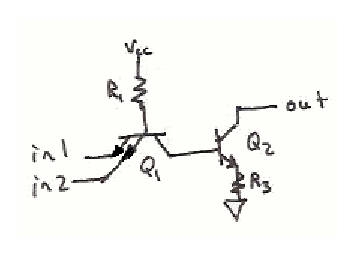
\includegraphics{images/TTLnand_opencollector.eps}
\end{center}
\end{figure}

\subsection{Totem Pole Outputs}
Instead of trying to take advantage of wired logic through a pull-up, we could consider how can we make the outputs switch as fast as possible.  To do this we would need to pull up and down with separate transistors, so that we could quickly drive the output high or low.  This is what totem pole outputs does.  It is called totem pole outputs because the output transistors are on top of each other like a totem pole.

\begin{figure}
\begin{center}
\caption{Transistor Transistor Logic \textbf{Nand} Gate with Totem Pole Output.}\label{f:TTL_nand_totem}
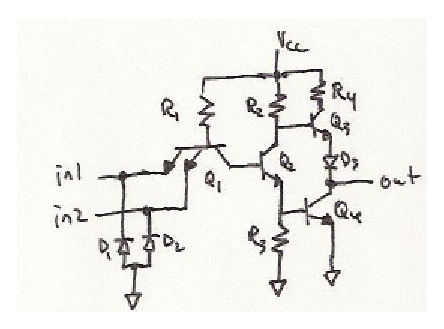
\includegraphics{images/TTLnand_totempole.eps}
\end{center}
\end{figure}

\subsection{Tristate Outputs}

\begin{figure}
\begin{center}
\caption{Transistor Transistor Logic \textbf{Nand} Gate with Tristate Output.}\label{f:TTL_nand_tristate}
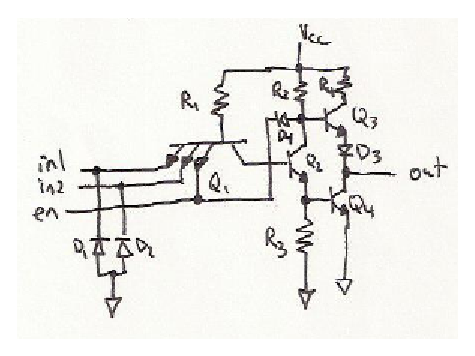
\includegraphics{images/TTLnand_tristate.eps}
\end{center}
\end{figure}




\section{CMOS Families}

\section{Static CMOS}

Static CMOS is the basic type, and aims at reliable, robust circuits.

\section{Dynamic CMOS}

Dynamic CMOS is designed to be small, fast, and low power.  Examples include PE Logic and Domino Logic, and require timing.  The key idea is to precharge and time the discharge to ensure that transitions occur quickly.  For instance Domino logic includes an inverter between gates to quickly change and cause a ripple of discharges from one stage to the next, thus falling like dominos\footnote{Yes dominos like the tile game, not the fast, cheap pizza. :)}.

\section{Interfacing}

There are a lot of logic families out there so I will only cover the most common ones in this section, the rest can be handled in similar ways, you just need to know the standard considerations of voltages (not just min and max but also the logic levels), current (input and output at high and low levels), impedance (not always needed but can be important on bus lines and such), floating outputs (high, low, or not at all), timing (rise time, fall time, latency, etc.), and data rates (really this is an implication of timing, but it is big enough to be mentioned separately).  It is helpful to know if the circuits you are interfacing are switching ground or power, as you can make a more reliable circuit using this information (i.e. you do the same in your circuit, which will be more compatible and thus also more reliable as it will not run into as many glitches caused by misreading a voltage level.).  The basic requirements to call two chips compatible are:

\begin{tabular}{rcl}
Driver Output  && Load Input \\
$V_{OH_{max}}$ & $<$ & $V_{IH_{max}}$\\
$V_{OH_{min}}$ & $>$ & $V_{IH_{min}}$\\
$V_{OL_{max}}$ & $<$ & $V_{IL_{max}}$\\
$V_{OL_{min}}$ & $>$ & $V_{I_{min}}$\\
$-I_{OH_{max}}$ & $>$ & $I_{IH_{max}}$\\
$I_{OL_{max}}$ & $>$ & $-I_{IL_{max}}$\\
\end{tabular}

The first two rows require that the high (true in positive logic) output voltage range must be contained in the high input voltage range, so that any $H$ produced is correctly received.  The next two lines do the same thing for the low values.  The last two are to ensure that the driving chip can supply the needed current for a $H$ and sink the needed current for a $L$.  Note the negative signs are present because they flow out of the corresponding terminals rather than in.  Level shifters can be placed between to meet voltage requirements, or current amplifiers/buffer stages can be used to meet current requirements.  Typically, the first requirement is met by keeping the supply voltage the same, provided they can both take the same supply voltage.  Similarly the fourth requirement is met by providing both the same ground.  The last two requirements need to be verified for the entire load they are driving (fan-out and fan-in problems).

Before you design a circuit to interface, you should check if there is a device that already does the interfacing.  In many cases there are devices designed for interfacing.  For instance, between the old TTL family and the newer CMOS families (C, HC, AC, ACH, etc.), there are T versions (CT, HCT, ACT, ACHT, etc.) that can drop in replace the old TTL components, or one of the T devices can sit between the families and convert (say a buffer or two inverters).  This is by far the easiest way to do the conversion, and I would do it this way unless forced to do otherwise.  It is useful to know how to convert, should you ever have to, so below are the basics.

If you are straight converting signals, you often want to go through two inverters\footnote{The inverters buffer the input.  Don't use an actual buffer because a buffer is slower than an inverter, so buffers should be avoided unless absolutely needed.  Basically, you put an inverter of the same logic type of the output immediately after the output and an inverter of the same logic type as the input immediately before the input.}, as these devices as they are often used for this purpose, they are frequently designed to handle input and output.  Note that you do not have to use inverters, they are a protection layer.  The inverters serve as sacrificial elements (one for each logic family) to protect the circuits they are interfacing.  Frequently you put them and any other interfacing hardware on a shim board, then if anything gets damaged it is the shim, not the original circuit.

Let's pick up the case mentioned above, where we wanted to go from an old TTL output to a newer CMOS input (say from a 74LS to a 74HC), but assume for some reason, we didn't just want to us a 74HCT to interface.  We would need three circuit elements: a but would also need a pull up resistor of about 1k between them for two reasons.  First, the voltage levels are incompatible, particularly at the high range, and the pull up solves this.  Second, the pull up resistor is used to guarantee the input does not stay in the dangerous 0.8v to 2.0v range\footnote{In the transition voltage range the P-channel to Vcc and the N-channel to ground can both be open, creating a path from Vcc to ground.  This causes a current spike which can damage circuits if it is around too long.  This happens every transition between high and low, but in the new CMOS families transitions are so fast the time of current spike is thus so short it does not effect things. The TTL output is slower and thus can allow significant damage.  A pull up (or pull down if you want the default low) resistor solves this problem.}.  To calculate the pull-up resistor more precisely you can use
\begin{eqnarray}
R_{pull-up} &\geq& \frac{V_{cc}max-V_{TTL\; Low\; Output}}{I_{TTL\; Low\; Output} + (num\; inputs)I_{CMOS\; Low\; Input}}\label{eq-resistor-pull-up-min}\\
R_{pull-up} &\leq& \frac{V_{cc}-V_{CMOS\; Input\; High}}{(num\; inputs)I_{CMOS\; Input\; High}}\label{eq-resistor-pull-up-max}
\end{eqnarray}
Usually the minimum value is in the mid to high hundreds so a 1k resistor is a good guess up till about $num\; inputs=8$, past that I would guess 2k till about $num\; inputs=16$, I would not drive more than 16 gates directly with anything at the moment (theoretically you can but current, heat, and transients become big problems).  The input current of CMOS devices is very small, so it can usually be ignored in the lower bound, and will cause the upper bound to be large (but finite).  As the number of devices grows it cannot be ignored and at around $num\; inputs=18$ there is a crossover, thus no pull-up resistor will work.  You should calculate the minimum and maximum for any problem to ensure there is a feasible region and you are in it.

Depending on the circuit, you might also have to guarantee a particular rise time (the second reason we wanted a pull-up).  In this case we have a simple first order\footnote{This is the solution of a first order derivative equation for the rise time of a driven RC circuit.  Theoretically they covered a lot of this in your physics sequence.} equation
\begin{eqnarray}
V_{CMOS\; Input\; High} &=& V_{CC}\left(1-e^{-\frac{t}{C\cdot R_{pull-up}}}\right)
\end{eqnarray}
where $t$ is the desired rise time, and $C$ is the total capacitance of the circuit, which is the sum of the output capacitance of the driving circuit, the input capacitance of the receiving circuits, and the capacitance of the line (often negligible but not always, it is probably about 1pF/cm).  You can solve this for the value of $R_{pull-up}$.  All of this assumed open-collector output (nothing driving high).  If something is driving the circuit high, the pull-up resistor only has to account for the missing voltage.  For instance totem pole output (typical for many TTL such as the LS family logic gates) is driven to at least 2.7 volts in around 10ns.  Given some driven output voltage the equation for the pull-up resistor is
\begin{eqnarray}
V_{CMOS\; Input\; High}-V_{Driven\; Output} &=& (V_{CC}-V_{Driven\; Output})\left(1-e^{-\frac{t}{C\cdot R_{pull-up}}}\right).
\end{eqnarray}
Again solve for $R_{pull-up}$ and then ensure it falls between the minimum (Eq.~\ref{eq-resistor-pull-up-min}) and maximum (Eq.~\ref{eq-resistor-pull-up-max}).

If we were going the other way, we could just directly connect them, as long as we were in the fan-out restrictions, which is at least 10 gates for LS-TTL or 2-4 gates for TTL.  Often designers put an additional CMOS buffer, say a 4096, for timing input to the slower TTL circuits.  Note the data rates must be compatible, or no buffer will be able to solve incompatible data rates for continuous data streams.

As an interesting side note TTL at 5v is directly compatible, both ways with CMOS at 3v.  Fan in and out restrictions still apply.

It is worth noting that CMOS has a wide range of voltage operation, so it is not uncommon to have to convert voltage ranges.  Resistor voltage dividers are common for going down, and amplifier circuits, such as an open drain CMOS device with a pull-up resistor.  As a particularly interesting case is ECL, which is usually run between 0v and -5.2v so the voltage differences and potential logic inversions need to be handled, or you can just run the CMOS from the same supply, and then just use diodes on the interface for protection. 
\part{Digital Logic}
\input{Kohw_boolean}
\chapter{Logic Conventions}

In a standard digital logic course, a usual starting point is to associate a high voltage, say 5v or 3.3v, with true (1), and a low voltage, usually ground, with false (0).  The purpose of this chapter is to blow that assumption out of the water.  We really have two completely different things we need to associate some way.  One is a system of logic, composed of truth (1), falsehood (0)\footnote{These associations of true with 1 and false with 0 are conventions also, and we could play with them also, but we will leave that off to a discussion of math for another book.}, and logical gates.  The other system is a physical one of high voltages (Vcc or Vdd), low voltages (ground), and hardware devices that operate off these voltage values.

Ideally we would like a system that allows us to look at the logic without having to think about the hardware, or to look at the hardware without thinking about the logic.  Mixed logic allows us to do this.  To use it we will design the logic as we normally would, without any thought of the hardware that we will use to implement.  When we go to select the devices to implement the logic gates, we will use mixed logic to give us flexibility in the selection of devices, by strategically and consistently changing the logic convention in place at different locations in our design.  As long as we do this we will not change the logic of our design.

I need to take a little pedantic aside, because the term logic convention, which is standardly used to refer to the association of logic values to voltage values has an unintended implication that seems to confuse people. Logic convention causes people to think that the voltages are preserved but the logic is changing, which is no problem for analysis but causes unnecessary confusion in design.  We could have used the term voltage convention to refer to the same think because it is a design oriented term, i.e. it does not suggest you are changing your logic, you are changing your voltage associations, but then people would get confused in design.  Once you become used to a term you are fine, but it is the learning I care about, and it is for this reason I suggest logic-voltage convention (LVC). LVC does not have any connotation toward design or analysis, and thus I hope will cause people to understand it better and use it more.

\section{Logic-Voltage Conventions}

The first LVC is positive logic, which is what most digital logic students think is the only one there is.  Positive logic is also called active-high, which is more in keeping with my pedantic aside from the introduction.  See Table~\ref{tab:positive_logic}.

\begin{table}\begin{center}
\caption{Positive Logic/Active-High}\label{tab:positive_logic}
\begin{tabular}{cc}
Logic & Voltage \\\hline
F     & L \\
T     & H \\
\end{tabular}
\end{center}\end{table}

The second LVC is negative logic, which becomes important in developing the other two canonical forms in Section~\ref{s-canonical}.  Negative logic is also called active-low, which is more in keeping with my pedantic aside from the introduction.  See Table~\ref{tab:negative_logic}.

\begin{table}\begin{center}
\caption{Negative Logic/Active-Low}\label{tab:negative_logic}
\begin{tabular}{cc}
Logic & Voltage \\\hline
F     & H \\
T     & L \\
\end{tabular}
\end{center}\end{table}

The final LVC is mixed logic, which uses either positive or negative logic rules on a wire by wire basis.  The key to using this is to have a system of marking the wires and the signal names so you can tell which convention is in place.
\begin{itemize}
\item The traditional way to mark wires for positive logic (active-high) was to do nothing, i.e. just draw the wire.  The new (from 1984) IEEE standard has us put a flag on  top of the wire at each end that points in the direction of flow (into the device for inputs, out of the device for outputs), and is associated with the term active-high.  The flags look like a small right triangle with the base formed by the wire and the hypotenuse pointing in the direction of the flow.
\item Positive logic wire/signal names have a `.H' or `.h' appended to it.  Some people append either a `$+$' or a `$\uparrow$' but I find this more tedious.  A final convention puts a lower case p in front.  In other cases nothing is added to the name for these, and the absence lets you know the convention, though this is error prone as you can't tell if the signal was just missed in the naming.  I suggest you use the `.h' to be clear.
\item Wires that use the negative logic convention have an open circle on all ends with the classic logic shapes.  Active-low flags (open arrow, only on the lower part, pointing in the direction of signal travel) are used interchangeably with negative logic bubbles, though you should pick a convention and stick with it.  The flags look like a small right triangle with the base formed by the wire and the hypotenuse pointing in the direction of the flow.
\item Negative logic (active-low) name/signal has a `.L' appended.  Some people also append: a `$-$', a `$\downarrow$', a `\#'.  Other notations put leading symbols of a `n' or a slash, `/', which is designed to look like an bar over the signal, which is the final way.  I don't like the overbar or slash as it is easily confused with not, though it is the most common\footnote{It is an inconsistent use of the bubbles and slashes that causes so much confusion in digital logic students, so I will avoid them.  Hopefully when you feel comfortable with the conventions you will then have no problem reading the highly overloaded syntax that is commonly used.}.  The `\verb1_B1' notation is confusing as it could mean byte in other contexts.
\end{itemize}
In general the bubbles go with the classic logic shapes, and the arrows go with the new IEEE 91-1984 standard, which calls for boxes with symbols.  Mixed logic is much more flexible in the ability to use other hardware devices to implement gates.  One way of thinking of this is that we can implement a logic function with a variety of hardware devices, or put the other way one hardware device can implement a variety of logic gates.  This is easiest to explain by an example.

\begin{example}
Say we need a `not' gate. With either positive or negative logic we have only one choice, but consider mixed logic.  We could have the input as either positive or negative and a similar but independent choice for the output.  This means we have four possible mixed conventions.  But how many devices? Is this only an illusion of choice?
\begin{enumerate}
\item Positive logic to positive logic

\begin{tabular}{cc||cc}
Logic In & Voltage In & Voltage Out & Logic Out \\\hline
F        & L          & H           & T         \\
T        & H          & L           & F         \\
\end{tabular}

This requires a voltage inverter, which is what most people think a `not' gate is.

\item Negative logic to negative logic

\begin{tabular}{cc||cc}
Logic In & Voltage In & Voltage Out & Logic Out \\\hline
F        & H          & L           & T         \\
T        & L          & H           & F         \\
\end{tabular}

This also requires a voltage inverter, so no new requirement is added.

\item Positive logic to negative logic

\begin{tabular}{cc||cc}
Logic In & Voltage In & Voltage Out & Logic Out \\\hline
F        & L          & L           & T         \\
T        & H          & H           & F         \\
\end{tabular}

The voltage is already correct so only a wire is needed to connect them.  We now have something new, a `bare wire not'.  Think about this for a second, we have a wire that can do logical negation.  That is pretty cool.

\item Negative logic to positive logic

\begin{tabular}{cc||cc}
Logic In & Voltage In & Voltage Out & Logic Out \\\hline
F        & H          & H           & T         \\
T        & L          & L           & F         \\
\end{tabular}

Again the voltages are correct so only a wire is needed.
\end{enumerate}
Our four logic combinations gave us two different devices (inverter or bare wire) that could fulfil our needs, depending on the convention picked.   That is one more than with either straight positive logic or straight negative logic, which yielded the same one possibility (inverter) as each other.  The increased design flexibility is important in a real design situation.
\end{example}

Now lets try from a different perspective.  The last example started with a requirement on the logic and found what devices could work, now let's start with the device and find out what it can do for our logic.

\begin{example}
The voltage characteristics of an inverter is

\begin{tabular}{cc}
Voltage In & Voltage Out \\\hline
L          & H           \\
H          & L           \\
\end{tabular}

Now we just have to add the interpretation, i.e. the logic convention.  We have four possibilities for a single input, single output.
\begin{enumerate}
\item Positive logic to positive logic

\begin{tabular}{cc||cc}
Logic In & Voltage In & Voltage Out & Logic Out \\\hline
F        & L          & H           & T         \\
T        & H          & L           & F         \\
\end{tabular}

This is `not', and as we noted in the last example this is why most people think an inverter is `not'.

\item Negative logic to negative logic

\begin{tabular}{cc||cc}
Logic In & Voltage In & Voltage Out & Logic Out \\\hline
F        & H          & L           & T         \\
T        & L          & H           & F         \\
\end{tabular}

This also is `not'.

\item Positive logic to negative logic

\begin{tabular}{cc||cc}
Logic In & Voltage In & Voltage Out & Logic Out \\\hline
F        & L          & H           & F         \\
T        & H          & L           & T         \\
\end{tabular}

This is a logic convention changer.  It preserves the interpretation (logic value) but switches conventions.

\item Negative logic to positive logic

\begin{tabular}{cc||cc}
Logic In & Voltage In & Voltage Out & Logic Out \\\hline
F        & H          & H           & T         \\
T        & L          & L           & F         \\
\end{tabular}

Again the we see the inverter also `inverts' the convention.
\end{enumerate}
We thus have that an inverter can serve one of two purposes: logic value inversion (not) or logic convention inversion (converter).
\end{example}

The options are even larger with two input gates.

\begin{example}
Consider an `\textbf{andn}' gate in positive logic.  What could we use to make it with standard TTL Gates (\textbf{nand}, \textbf{nor}, \textbf{and}, \textbf{or}, \textbf{not}, \textbf{xor}, \textbf{xnor})?

Answer:

Let's start by looking at the logic table of an \textbf{andn} gate.

\begin{tabular}{c|c||c}
A & B & A andn B \\\hline
0 & 0 & 0 \\
0 & 1 & 0 \\
1 & 0 & 1 \\
1 & 1 & 0 \\
\end{tabular}

Since this is positive logic, we have to find a device or devices that give us the voltage pattern below.

\begin{tabular}{c|c||c}
In 1 & In 2 & Out \\\hline
L    & L    & L \\
L    & H    & L \\
H    & L    & H \\
H    & H    & L \\
\end{tabular}

\begin{enumerate}
\item If we used positive logic everywhere, we would have an \textbf{andn} gate, which we have no implementation for directly, so we could use an \textbf{not} on in2(B) and then \textbf{and} the result with in1(A).

\begin{tabular}{c|c||c}
A & $\bar{B}$ & A and $\bar{B}$ \\\hline
0 & 1 & 0 \\
0 & 0 & 0 \\
1 & 1 & 1 \\
1 & 0 & 0 \\
\end{tabular}

\item If we used negative logic on in2, we would have an \textbf{and} gate, and we could use an inverter (\textbf{not}) to take the initial positive logic system on in2 to make it negative logic without negating the input.

\begin{tabular}{c|c||c}
A & B.L & A and B.L \\\hline
0 & 1 & 0 \\
0 & 0 & 0 \\
1 & 1 & 1 \\
1 & 0 & 0 \\
\end{tabular}
\item If we used negative logic on in1, we would have a \textbf{nor} gate, and we could use an inverter (\textbf{not}) to take the initial positive logic system on in1 to make it negative logic without negating the input.

\begin{tabular}{c|c||c}
A.L & B & A.L nor B \\\hline
1 & 0 & 0 \\
1 & 1 & 0 \\
0 & 0 & 1 \\
0 & 1 & 0 \\
\end{tabular}

\item If we used negative logic on both inputs, we would have a norn gate, which is not implemented.  The negation of B.L can be handled by a bare wire not, which will also work to go from B.h to$\not$B.L.  Going from A.h to A.L can be handled by an inverter (\textbf{not}).  The rest can be handled by a \textbf{nor} gate, so that this is the same as the last case.

\begin{tabular}{c|c||c}
A.L & B.L & A.L norn B.L \\\hline
1 & 1 & 0 \\
1 & 0 & 0 \\
0 & 1 & 1 \\
0 & 0 & 0 \\
\end{tabular}

\item If we used negative logic only on the output we would have nandn, which is not implemented.  We need a \textbf{not} on in2, and a bare wire not on the output handling the logic level and not of the output, leaving the main gate as an \textbf{and}.

\begin{tabular}{c|c||c}
A & B & (A nandn B).L \\\hline
0 & 0 & 1 \\
0 & 1 & 1 \\
1 & 0 & 0 \\
1 & 1 & 1 \\
\end{tabular}

\item If we used negative logic on in2 and the output, we would have an \textbf{nand} gate, and we could use an inverter (\textbf{not}) to take the initial positive logic system on in2 to make it negative logic without negating the input and similarly an inverter (\textbf{not}) could be used to take the initial negative logic output and convert to positive logic.

\begin{tabular}{c|c||c}
A & B.L & (A nand B.L).L \\\hline
0 & 1 & 1 \\
0 & 0 & 1 \\
1 & 1 & 0 \\
1 & 0 & 1 \\
\end{tabular}
\item If we used negative logic on in1 and the output, we would have a \textbf{or} gate, and we could use an inverter (\textbf{not}) to take the initial positive logic system on in1 to make it negative logic without negating the input and similarly an inverter (\textbf{not}) could be used to take the initial negative logic output and convert to positive logic.

\begin{tabular}{c|c||c}
A.L & B & (A.L or B).L \\\hline
1 & 0 & 1 \\
1 & 1 & 1 \\
0 & 0 & 0 \\
0 & 1 & 1 \\
\end{tabular}
\item If we used negative logic on both inputs and the output, we would have \textbf{orn}, which does not exist.  We could make it by using a bare wire not on in2 and inverters (\textbf{not}) on in1 and the output.  The main gate is now an \textbf(or).

\begin{tabular}{c|c||c}
A.L & B.L & (A.L or B.L).L \\\hline
1 & 1 & 1 \\
1 & 0 & 1 \\
0 & 1 & 0 \\
0 & 0 & 1 \\
\end{tabular}
\end{enumerate}

The above cases reduce to four possibilities:
\begin{enumerate}
\item an \textbf{and} with a \textbf{not} on in2,
\item an \textbf{nor} with a \textbf{not} on in1,
\item an \textbf{nand} with a \textbf{not} on in2 and output,
\item an \textbf{or} with a \textbf{not} on in1 and output.
\end{enumerate}
It is straightforward to show they are equivalent, the nice thing is that mixed logic can generate them all.
\end{example}

It is this flexibility is one great reason that mixed logic so popular.


\section{Canonical Forms}\label{s-canonical}

Only in rare cases are problems easy enough to reduce to a single gate we can recognize.  In most cases we need to design more complicated circuits to achieve the desired result.  An important result in boolean logic is that every possible output pattern can be realized from input signals in two levels of logic if each gate can have as many inputs as you need.  The practical use of this is that we can create canonical forms.  Two main canonical forms are used, Sum-of-Products (SOP) and Product-of-Sums (POS).  Each canonical is made up of terms, and each term corresponds to one row of a truth table.  Since each term corresponds to a row in the truth table the terms can be referenced by the row number or the actual equation for the term (I will show how to get the equations below)  The names were designed to be descriptive, as follows.

\subsection{Sum of Products}

A sum is a series of terms connected by ``+'', which is \textbf{or} in our case.  A product is a series of terms connected by ``$\cdot$'', which is \textbf{and} in our case, thus SOP is bunch of terms that only use \textbf{and} in them that are connected together by \textbf{or}.  We call each term in a SOP a Miniterm because it is only true for one combination of inputs (since \textbf{and} is only true for one combination of inputs this follows directly).  In essence each Miniterm places one true (1) value in the output, and thus can be thought of as tracking the 1's.  Each Miniterm's equation is written such that it will be true for that row only of the truth table.  Consider the following.

\vspace{.1in}
\begin{tabular}{c|c|c|cl}
x & y & z & Row & Miniterm   \\ \hline
0 & 0 & 0 & 0   & $x'\cdot y'\cdot z'$ \\
0 & 0 & 1 & 1   & $x'\cdot y'\cdot z$  \\
0 & 1 & 0 & 2   & $x'\cdot y\cdot z'$  \\
0 & 1 & 1 & 3   & $x'\cdot y\cdot z$   \\
1 & 0 & 0 & 4   & $x\cdot y'\cdot z'$  \\
1 & 0 & 1 & 5   & $x\cdot y'\cdot z$   \\
1 & 1 & 0 & 6   & $x\cdot y\cdot z'$   \\
1 & 1 & 1 & 7   & $x\cdot y\cdot z$    \\
\end{tabular}
\vspace{.1in}

Notice that the row number is just the decimal value of binary number (xyz).  Also note that the Miniterm is formed by placing complements where the corresponding variable is zero, this forces all the variables (or complements) to be true for the equation on that row.  To get a better appreciation of what it means for a Miniterm to be adding or tracking the 1's consider a series of truth tables.

\vspace{.1in}
\noindent
\begin{tabular}{p{1.1in}p{1.5in}p{1.6in}p{1.4in}}
$a_1=x\cdot y\cdot z$ & $a_2=x\cdot y\cdot z+x\cdot y'\cdot z$ &
$a_3=x\cdot y\cdot z+x\cdot y'\cdot z+x\cdot y'\cdot z'$ &
$a_4=x\cdot y\cdot z+x\cdot y'\cdot z+x\cdot y'\cdot z'+x'\cdot y\cdot z'$ \\
\begin{tabular}{c|c|c|c}
x & y & z & a \\ \hline
0 & 0 & 0 & 0 \\
0 & 0 & 1 & 0 \\
0 & 1 & 0 & 0 \\
0 & 1 & 1 & 0 \\
1 & 0 & 0 & 0 \\
1 & 0 & 1 & 0 \\
1 & 1 & 0 & 0 \\
1 & 1 & 1 & 1 \\
\end{tabular}
&
\begin{tabular}{c|c|c|c}
x & y & z & a \\ \hline
0 & 0 & 0 & 0 \\
0 & 0 & 1 & 0 \\
0 & 1 & 0 & 0 \\
0 & 1 & 1 & 0 \\
1 & 0 & 0 & 0 \\
1 & 0 & 1 & 1 \\
1 & 1 & 0 & 0 \\
1 & 1 & 1 & 1 \\
\end{tabular}
&
\begin{tabular}{c|c|c|c}
x & y & z & a \\ \hline
0 & 0 & 0 & 0 \\
0 & 0 & 1 & 0 \\
0 & 1 & 0 & 0 \\
0 & 1 & 1 & 0 \\
1 & 0 & 0 & 1 \\
1 & 0 & 1 & 1 \\
1 & 1 & 0 & 0 \\
1 & 1 & 1 & 1 \\
\end{tabular}
&
\begin{tabular}{c|c|c|c}
x & y & z & a \\ \hline
0 & 0 & 0 & 0 \\
0 & 0 & 1 & 0 \\
0 & 1 & 0 & 1 \\
0 & 1 & 1 & 0 \\
1 & 0 & 0 & 1 \\
1 & 0 & 1 & 1 \\
1 & 1 & 0 & 0 \\
1 & 1 & 1 & 1 \\
\end{tabular} \\
\end{tabular}
\vspace{.1in}

Each time a term is added the truth table shows the output in the corresponding row to the new term becomes 1.  It is thus evident that we can go the reverse direction.  We always want a shorter way to write things, so since Miniterm implies small we can also represent the term by a small "m" followed by the row number, so $m_5=x\cdot y'\cdot z$.  Using this notation the designs above are $a_1=\{m_7\}$, $a_2=\{m_5,\,m_7\}$, $a_3=\{m_4,\,m_5,\,m_7\}$, and $a_4=\{m_2,\,m_4,\,m_5,\,m_7\}$.

This is nice and short but we want even shorter so we abbreviate the list of Miniterms by $\sum$ followed by a list of the numbers of the terms (you might recall that $\sum$ means a series of '$+$' in math).  While it is not a general rule, I list the inputs as subscripts of $\sum$, it makes it easier to tell the sequence and what signals (wires) to connect.  Thus our summation notation for the designs would be, $a_1=\sum_{x,y,z}(7)$, $a_2=\sum_{x,y,z}(5,7)$, $a_3=\sum_{x,y,z}(4,5,7)$, and $a_4=\sum_{x,y,z}(2,4,5,7)$.  Note the listing of inputs as subscripts can be done with the listing of Miniterms, $a_1=\{m_7\}_{x,y,z}$, $a_2=\{m_5,\,m_7\}_{x,y,z}$, $a_3=\{m_4,\,m_5,\,m_7\}_{x,y,z}$, and $a_4=\{m_2,\,m_4,\,m_5,\,m_7\}_{x,y,z}$.


\subsection{Product of Sums}
By the colloquial descriptions above for sum and product, POS is a bunch of terms that only use \textbf{or} gates internally and are connect by \textbf{and} gates.  We call each term in a POS a Maxiterm because it is true for every input combination but one (since it is made of \textbf{or} gates).  A Maxiterm is thus false for only one combination of the inputs.  In essence each Maxiterm places one false (0) value in the output, so it can be thought of as tracking the 0's.  Each Maxiterm's equation is written such that it will be true for that row only of the truth table.  Consider the following.

\vspace{.1in}
\begin{tabular}{c|c|c|cl}
x & y & z & Row & Maxiterm   \\ \hline
0 & 0 & 0 & 0   & $x+y+z$    \\
0 & 0 & 1 & 1   & $x+y+z'$   \\
0 & 1 & 0 & 2   & $x+y'+z$   \\
0 & 1 & 1 & 3   & $x+y'+z'$  \\
1 & 0 & 0 & 4   & $x'+y+z$   \\
1 & 0 & 1 & 5   & $x'+y+z'$  \\
1 & 1 & 0 & 6   & $x'+y'+z$  \\
1 & 1 & 1 & 7   & $x'+y'+z'$ \\
\end{tabular}
\vspace{.1in}

Notice that the row number is just the decimal value of binary number (xyz).  Also note that the Maxiterm is formed by placing complements where the corresponding variable is one, this forces all the variables (or complements) to be false for the equation on that row.    To get a better appreciation of what it means for a Maxiterm to be adding or tracking the 0's consider a series of truth tables.

\vspace{.1in}
\noindent
\begin{tabular}{p{1.1in}p{1.5in}p{1.6in}p{1.4in}}
$\bar a_1=(x+y+z)$ & $\bar a_2=(x+y+z)\cdot(x+y+z')$ &
$\bar a_3=(x+y+z)\cdot(x+y+z')\cdot(x+y'+z')$ &
$a_4=(x+y+z)\cdot(x+y+z')\cdot(x+y'+z')\cdot(x'+y'+z)$ \\
\begin{tabular}{c|c|c|c}
x & y & z & a \\ \hline
0 & 0 & 0 & 0 \\
0 & 0 & 1 & 1 \\
0 & 1 & 0 & 1 \\
0 & 1 & 1 & 1 \\
1 & 0 & 0 & 1 \\
1 & 0 & 1 & 1 \\
1 & 1 & 0 & 1 \\
1 & 1 & 1 & 1 \\
\end{tabular}
&
\begin{tabular}{c|c|c|c}
x & y & z & a \\ \hline
0 & 0 & 0 & 0 \\
0 & 0 & 1 & 0 \\
0 & 1 & 0 & 1 \\
0 & 1 & 1 & 1 \\
1 & 0 & 0 & 1 \\
1 & 0 & 1 & 1 \\
1 & 1 & 0 & 1 \\
1 & 1 & 1 & 1 \\
\end{tabular}
&
\begin{tabular}{c|c|c|c}
x & y & z & a \\ \hline
0 & 0 & 0 & 0 \\
0 & 0 & 1 & 0 \\
0 & 1 & 0 & 1 \\
0 & 1 & 1 & 0 \\
1 & 0 & 0 & 1 \\
1 & 0 & 1 & 1 \\
1 & 1 & 0 & 1 \\
1 & 1 & 1 & 1 \\
\end{tabular}
&
\begin{tabular}{c|c|c|c}
x & y & z & a \\ \hline
0 & 0 & 0 & 0 \\
0 & 0 & 1 & 0 \\
0 & 1 & 0 & 1 \\
0 & 1 & 1 & 0 \\
1 & 0 & 0 & 1 \\
1 & 0 & 1 & 1 \\
1 & 1 & 0 & 0 \\
1 & 1 & 1 & 1 \\
\end{tabular} \\
\end{tabular}
\vspace{.1in}

Notice that each time a term is added the truth table shows the output in the corresponding row to the new term becomes 0.  It is thus evident that we can go the reverse direction.  We always want a shorter way to write things, so since Maxiterm implies large we can also represent the term by a capital "M" followed by the row number, so $M_5=x'+y+z'$.  Using this notation the designs above are $\bar a_1=\{M_0\}$, $\bar a_2=\{M_0,\,M_1\}$, $\bar a_3=\{M_0,\,M_1,\,M_3\}$, and $a_4=\{M_0,\,M_1,\,M_3,\,M_6\}$.

This is nice and short but we want even shorter so we abbreviate the list of Maxiterms by $\prod$ followed by a list of the numbers of the terms (you might recall that $\prod$ means product in math).  While it is not a general rule, I list the inputs as subscripts of $\prod$, it makes it easier to tell the sequence and what signals (wires) to connect.  Thus our product notation for the designs would be, $\bar a_1=\prod_{x,y,z}(0)$, $\bar a_2=\prod_{x,y,z}(0,1)$, $\bar a_3=\prod_{x,y,z}(0,1,3)$, and $a_4=\prod_{x,y,z}(0,1,3,6)$.  Note the listing of inputs as subscripts can be done with the listing of Maxiterms, $\bar a_1=\{M_0\}_{x,y,z}$, $\bar a_2=\{M_0,\,M_1\}_{x,y,z}$, $\bar a_3=\{M_0,\,M_1,\,M_3\}_{x,y,z}$, and $a_4=\{M_0,\,M_1,\,M_3,\,M_6\}_{x,y,z}$.

As a final note, the last problem in this section is the same as the last one in the SOP section and so the designs must be equivalent.  We thus have $a_4=\prod_{x,y,z}(0,1,3,6)=\sum_{x,y,z}(2,4,5,7)$, from which we can note that the if we take all the numbers from the truth table and remove the ones from the $\prod$ list, we have the $\sum$ list and vice versa.  This gives us a nice way to switch between the two forms provided we know how many rows are in the table, which you can know from counting the number of inputs in our subscript (another good reason for listing them).



\vspace{6pt}
\textbf{Example}
\vspace{6pt}

Obtain the sum of products form by algebra and the product of
sums form by truth table for $A+B\cdot (C + A)\cdot(B'+ A'\cdot B)$.

\beqn
A+B\cdot (C + A)\cdot(B'+ A'\cdot B)
& = & A+B\cdot(B'+ A'\cdot B)\cdot (C + A) \\
& = & A+(B\cdot B'+ B\cdot A'\cdot B)\cdot (C + A) \\
& = & A + A'\cdot B \cdot (C + A) \\
& = & A + A'\cdot B \cdot C + A'\cdot B \cdot A \\
& = & A + A'\cdot B \cdot C \\
& = & A\cdot(B+B')\cdot(C+C') + A'\cdot B \cdot C \\
& = & A\cdot B' \cdot C' + A\cdot B' \cdot C + A\cdot B \cdot C' + A\cdot B \cdot C + A'\cdot B \cdot C \\
& = & m_4 + m_5 + m_6 + m_7 + m_3 \\
& = & \Sigma(3,4,5,6,7)_{A,B,C}
\eeqn

\begin{tabular}{c|c|c||c}
A & B & C & $A+B\cdot (C + A)\cdot(B'+ A'\cdot B)$ \\
\hline
0 & 0 & 0 & 0 \\
0 & 0 & 1 & 0 \\
0 & 1 & 0 & 0 \\
0 & 1 & 1 & 1 \\
1 & 0 & 0 & 1 \\
1 & 0 & 1 & 1 \\
1 & 1 & 0 & 1 \\
1 & 1 & 1 & 1 \\
\end{tabular}

The three terms with 0's are thus $M_0$, $M_1$, and $M_2$, yielding $\Pi(0,1,2)_{A,B,C}$.


\input{Kohw_combinational}
\input{Kohw_sync}
\chapter{Timing}

\section{Combinational Circuits}

\karnaughmap{3}{f(a,b,c):}{acb}{10110010}{}




\section{Sequential Circuits}

The timing on sequential circuits revolves around ensuring that the setup and hold times of a flip flop are met in the circuit.  We will be using a bunch of different measurements of a circuit so we will begin by defining them.
\begin{description}
  \item[Trigger] The event which is used to start a sequential circuit, usually the rising or falling edge of a clock.
  \item[Setup time ($T_s$)] The minimum time the inputs must be stable before a trigger so the correct value is latched.  Failing to do so is a setup violation.
  \item[Hold time ($T_h$)] The minimum time the inputs must be stable after a trigger so the correct value is latched.  Failing to do so is a hold violation.
  \item[Clock period ($T_{clk}$)] The time between successive rising (or falling) edges in the clock signal.
  \item[Clock skew ($T_{skew}$)] The propagation time difference between furthest components, which thus is the time difference of them reading the same clock.  You can think of it as the time error range.
  \item[Flip Flop Clock propagation ($T_{clk-xmit}$)]  The time from when a flip flop receives the trigger till when the data is transmitted from it.  This is sometimes referred to as the time from clock to q.
  \item[Combinational Logic Delay ($T_{comb}$)] Time for a signal to pass through the combinational circuit.  Sometimes called \textbf{propagation delay}.
\end{description}

Now to ensure there is no problem in a sequential circuit, we must verify two conditions are met: the loop time in Eq.~\ref{eq:loop_timing}, and the arrival time in Eq.~\ref{eq:arrival_timing}.
\begin{eqnarray}
T_{clk} &\geq& T_s+T_{comb}+T_{clk-xmit}+T_{skew} \label{eq:loop_timing}\\
T_h     &\leq& T_{comb}+T_{clk-xmit}+T_{skew} \label{eq:arrival_timing}
\end{eqnarray}
Note that the loop time constrains the setup time, while the arrival time is a constraint on the hold time.  
\begin{itemize}
\item In a new design, you use the arrival time equation to determine the flip flop to use, and the loop time equation to determine the clock.
\item In an FPGA, you are stuck with the logic, flip flops, and the clock, so those parameters are fixed. The skew depends on position of the circuit elements (layout) is design dependent, so the equations are checked to verify a design.  If the design does not meet the clock timing an excessive skew warning is issued.
\end{itemize}

\section{Flip Flops and Hazards}

In Table~\ref{tab:metastabilitytimes7474}, I list the setup, hold, and the sum, which is the metastable interval or window.

\begin{table}
\caption{Interval when Metastability is most likely to occur}\label{tab:metastabilitytimes7474}
\begin{tabular}{lrrr}
Device   & $T_s$[ns] & $T_h$[ns] & $T_{ms}$ \\\hline
SN74LS74A        &	20   &	5    &	25\\
SN74ALS74A       &	15   &	0    &	15\\
SN74AS74A        &	4.5  &	0    &	4.5\\
SN74F74          &	3    &	1    &	4\\
CD74ACT74-Q1     &	4    &	0    &	4\\
SN54AHC74        &	5    &	0.5  &	5.5\\
SN54AHCT74       &	5    &	0    &	5\\
SN54LVC74A-SP    &	3    &	1    &	4\\
SN74AC74         &	3    &	0.5  &	3.5\\
SN74AC74-EP      &	3    &	0.5  &	3.5\\
SN74ACT74        &	3.5  &	1    &	4.5\\
SN74ACT74-EP     &	4    &	1    &	5\\
SN74AHC74        &	5    &	0.5  &	5.5\\
SN74AHC74-EP     &	5    &	0.5  &	5.5\\
SN74AHC74Q-Q1    &	5    &	0.5  &	5.5\\
SN74AHCT74       &	5    &	0    &	5\\
SN74AHCT74-EP    &	5    &	0    &	5\\
SN74AHCT74Q-Q1   &	5    &	0    &	5\\
SN74AUC74        &	0.7  &	0.3  &	1\\
SN74HC74         &	21   &	0    &	21\\
SN74HC74-EP      &	150  &	0    &	150\\
SN74HC74-Q1      &	17   &	0    &	17\\
SN74HCT74        &	14   &	0    &	14\\
SN74LV74A-EP     &	3    &	2.15 &	5.15\\
SN74LV74A-Q1     &	5    &	0.5  &	5.5\\
SN74LVC74A       &	3    &	0    &	3\\
SN74LVC74A-EP    &	3    &	1    &	4\\
SN74LVC74A-Q1    &	3    &	1    &	4\\
SN74S74          &	3    &	2    &	5\\
\end{tabular}
\end{table}




\section{How Often?}

Since the primary failure mode for entering metastability is a data change during setup and hold, the smaller these times the better, which means faster logic families.  The equations for calculating mean time between failures (MTBF) are

\begin{eqnarray}
MTBF
&=& \frac{e^{\frac{T_r}{T_{\gamma}}}}{F_dF_cT_p}\\
&=& \frac{e^{\frac{T_r+\frac{1}{F_c}-T_s}{T_{\gamma}}}}{F_dF_c^2T_p^2}
\end{eqnarray}

\begin{description}
\item[$F_d$] Data Frequency
\item[$F_c$] Clock Frequency
\item[$T_p$] Propagation delay of the flip flop
\item[$T_s$] Setup Time
\item[$T_r$] Resolve time (clock time minus the path time)
\item[$T_{\gamma}$] Resolution time of flip flop
\end{description}

\input{Kohw_async}
\input{Kohw_sysverilog}
\part{Data Representation and Manipulation}
\chapter{Codes}
\label{c-codes}

Codes are used to represent members of a set by a sequence of symbols.  For our purposes, the sequence of symbols will always be a sequence of $\{ 0,1\}$.  Codes have an encoding for each member to be represented. Codes can be fixed or variable in length. Fixed length codes like ascii have the same number of symbols in every encoding of the code.  Variable length codes use different numbers of symbols to represent the encodings.  For instance if '1' is 'a', '01' is 'b', and '00' is 'c', then the code is variable length.  The major trouble with variable length codes is splitting the message up into the individual encodings.  If the code is prefix (postfix) then the code can be directly read from left to right (right to left).

\section{Standard Codes}
\subsection{Unsigned}
\begin{tabular}{rcccccc}
decimal & Binary & Gray & BCD  & 2421 & Residue(5,3) & Residue(7,2) \\
0       & 0000   & 0000 & 0000 & 0000 & 000,00       & 000,0        \\
1       & 0001   & 0001 & 0001 & 0001 & 001,01       & 001,1        \\
2       & 0010   & 0011 & 0010 & 0010 & 010,10       & 010,0        \\
3       & 0011   & 0010 & 0011 & 0011 & 011,00       & 011,1        \\
4       & 0100   & 0110 & 0100 & 0100 & 100,01       & 100,0        \\
5       & 0101   & 0111 & 0101 & 1011 & 000,10       & 101,1        \\
6       & 0110   & 0101 & 0110 & 1100 & 001,00       & 110,0        \\
7       & 0111   & 0100 & 0111 & 1101 & 010,01       & 000,1        \\
8       & 1000   & 1100 & 1000 & 1110 & 011,10       & 001,0        \\
9       & 1001   & 1101 & 1001 & 1111 & 100,00       & 010,1        \\
10      & 1010   & 1111 &      &      & 000,01       & 011,0        \\
11      & 1011   & 1110 &      &      & 001,10       & 100,1        \\
12      & 1100   & 1010 &      &      & 010,00       & 101,0        \\
13      & 1101   & 1011 &      &      & 011,01       & 110,1        \\
14      & 1110   & 1001 &      &      & 100,10       & -            \\
15      & 1111   & 1000 &      &      & -            & -            \\
\end{tabular}

BCD is a decimal code designed to be compatible with standard binary numbers.  It is sometimes called 8421 code due to the weights on the columns.  The 2421 code was designed to be the same as BCD for 0-4 and make the 9's complement, which is important for easy subtraction, of 0-4 (i.e. 9-5 respectively) be easy to take because you can simply flip the bits.

Gray code is an alternate to binary.  It is not a decimal code, and hence does not waste 6 codes for every four bits.  Gray code was designed to have only one bit flip at any given time.  This is helpful in systems which have analog components and need to count.  For instance in an NC drill, we might want to encode the shaft position and hence put gray code bars on the shaft and have an ir sensor read them.  Since only one bit flips between each consecutive number, it is easy to verify if we are reading correctly and thus get a good idea of how fast the shaft is spinning and where the shaft is.  Gray code is also useful to us in Karnaugh maps and code maps because the one bit flipping property lets us find errors of type one easily (Karnaugh maps) and measure Hamming distance easily (code maps).  Notice that the first bit of a gray code is just like binary (all 0's first then 1's), while the rest follow a 0110 pattern on reducing scales.

The easiest way to read grey code is to start from the left and just copy the first bit.  From then on if the next digit to the right is 0 then repeat the last digit you wrote, if it is 1 flip the last digit you wrote.

\begin{example}
What is the value of $101111_{gray}$?

{\color{ans}
Starting at the left copy the first bit:

\begin{tabular}{l|cccccc}
Gray   & 1 & 0 & 1 & 1 & 1 & 1 \\ \hline
Binary & 1 &   &   &   &   &   \\
\end{tabular}

The next bit is a 0 so repeat the last bit you wrote (in this case a 1):

\begin{tabular}{l|cccccc}
Gray   & 1 & 0 & 1 & 1 & 1 & 1 \\ \hline
Binary & 1 & 1 &   &   &   &   \\
\end{tabular}

The next bit is a 1 so flip the last bit you wrote (in this case 1 flips to 0):

\begin{tabular}{l|cccccc}
Gray   & 1 & 0 & 1 & 1 & 1 & 1 \\ \hline
Binary & 1 & 1 & 0 &   &   &   \\
\end{tabular}

The next bit is a 1 so flip the last bit you wrote (in this case 0 flips to 1):

\begin{tabular}{l|cccccc}
Gray   & 1 & 0 & 1 & 1 & 1 & 1 \\ \hline
Binary & 1 & 1 & 0 & 1 &   &   \\
\end{tabular}

The next bit is a 1 so flip the last bit you wrote (in this case 1 flips to 0):

\begin{tabular}{l|cccccc}
Gray   & 1 & 0 & 1 & 1 & 1 & 1 \\ \hline
Binary & 1 & 1 & 0 & 1 & 0 &   \\
\end{tabular}

The next bit is a 1 so flip the last bit you wrote (in this case 0 flips to 1):

\begin{tabular}{l|cccccc}
Gray   & 1 & 0 & 1 & 1 & 1 & 1 \\ \hline
Binary & 1 & 1 & 0 & 1 & 0 & 1 \\
\end{tabular}

Binary 110101 is 53, so gray 101111 is 53.
}
\end{example}

Residue number systems (residue codes) are fun though rarely used because of the difficulty in converting back from them to binary.  Residue codes are specified by a series of remainders, taken to relatively prime bases (listed parenthesis and separated by commas).  The remainders are in the same order as the specified bases and also separated by commas.  The advantage of this system is you can perform fast addition, multiplication, and subtraction (if the divisor is not zero in any of the residues you can also do division efficiently), extremely fast, as the modulo terms are independently calculated by the modulo of the arithmetic operation being performed.

\begin{example}
Calculate $7+3$, $3*4$, $14-8$, and $14/7$ in Modulo(5,3).  Note we can do division because $7\mod 5=2>0$ and $7\mod 3 =1>0$.

{\color{ans}
$7+3 = (010,01) + (011,00) = (010+011 \mod 5,01+00 \mod 3) = (000,01) = 10$

$3*4 = (011,00)*(100,01) = (011*100 \mod 5, 00*01 \mod 3) = (010,00) = 12$

$14-8 = (100,10)-(011,10) = (100-011 \mod 5, 10 -10 \mod 3) = (001,00) = 6$

$14/7 = (100,10)-(010,01) = (100/010 \mod 5, 10/01 \mod 3) = (010,10) = 2$
}
\end{example}

\subsection{Signed}


\begin{tabular}{rlllll}
decimal & Signed Binary & 1's Comp  & 2's Comp & Excess-7 & Excess 8 \\
 8      & -             & -         & -        & 1111     & -        \\
 7      & 0111          & 0111      & 0111     & 1110     & 1111     \\
 6      & 0110          & 0110      & 0110     & 1101     & 1110     \\
 5      & 0101          & 0101      & 0101     & 1100     & 1101     \\
 4      & 0100          & 0100      & 0100     & 1011     & 1100     \\
 3      & 0011          & 0011      & 0011     & 1010     & 1011     \\
 2      & 0010          & 0010      & 0010     & 1001     & 1010     \\
 1      & 0001          & 0001      & 0001     & 1000     & 1001     \\
 0      & 0000,1000     & 0000,1111 & 0000     & 0111     & 1000     \\
-1      & 1001          & 1110      & 1111     & 0110     & 0111     \\
-2      & 1010          & 1101      & 1110     & 0101     & 0110     \\
-3      & 1011          & 1100      & 1101     & 0100     & 0101     \\
-4      & 1100          & 1011      & 1100     & 0011     & 0100     \\
-5      & 1101          & 1010      & 1011     & 0010     & 0011     \\
-6      & 1110          & 1001      & 1010     & 0001     & 0010     \\
-7      & 1111          & 1000      & 1001     & 0000     & 0001     \\
-8      & -             & -         & 1000     & -        & 0000     \\
\end{tabular}

Note that both signed binary and 1's compliment have a positive and negative 0.  Signed binary was an early development, but is not that useful because you can't use a standard adder/subtractor.

1's compliment is easy to calculate (flip the bits to convert from positive to negative), and is useful in turning an adder into a subtractor (the number to be subtracted is turned into the 2's complement, by finding the 1's complement, then setting the carry-in bit of the adder to do the $+1$).

2's compliment is the standard form for storing negative numbers in computers because you can easily convert (either by flipping bits and adding 1, or by starting on the right and copying bits up to and including the first 1, then flipping the remaining bits), and standard adder/subtractor circuits can be used.

Excess codes are most commonly used in floating point number exponents, as they preserve the numeric order of greatness (you can use standard compare circuits to check size).  The excess is either half the total numbers ($16/2=8$ for excess 8) or half the total numbers minus 1 ($16/2-1=7$ for excess 7).

\section{Huffman Codes}

Huffman codes are variable length codes that produce optimal expected code lengths.
\beqn
    ecl & = & \sum_{l\in C}\left( freq(l)\times length(l) \right)
\eeqn

\noindent Example:

Consider the string "adabaabcaabacadaccac" that we want to encode.  There are four members of the set (a, b, c, d) which means the members can be represented by a two bit fixed code.  But consider the following encoding (a=1, b=001, c=01, d=000).  The frequencies of the members are (a=10/20=.5, b= 3/20=.15, c=5/20=.25, d =2/20=.1). The ecl of the variable code is
\beqn
    ecl & = & .5*1 + .15*3 + .25*2 + .1*2 \\
        & = & 1.65
\eeqn
The expected code length is only 1.65 bits/character.

\subsection{Huffman Algorithm}
\begin{enumerate}
  \item Calculate the frequencies of each member
  \beqn
    \frac{\# \: occurrences \: of \: member}{Total \: occurrences}
  \eeqn
  \item Form decode tree from forest
    \begin{enumerate}
        \item make 1 node tree for each member with frequency and
        member name
        \item join two trees with the smallest frequency on root node by making them branches of a new root node and giving the new root node the sum of the frequencies of the old root nodes
        \item put new tree in forest and repeat joining till only
        one tree remains (the answer)
    \end{enumerate}
  \item encode or decode message
\end{enumerate}

\section{Error Detection and Correction}

Errors can happen in a variety of ways.  Bits can be added, deleted, or flipped.  Errors can happen in fixed or variable codes.  For simplicity we will consider only bit flips in fixed codes.  Note that variable codes can be packed into fixed length blocks for transmission and storage, so this is not as restrictive as it might sound at first.

The Hamming distance ($d_H$) between two codewords is the number of bit flips to turn one codeword into the other codeword.  It can also be thought of as the number of bits that are different between two codewords.  The Hamming distance can be extended to a set, by defining it as the minimum distance between any two codewords in the set.  The Hamming distance is useful in codes because it tells us how many errors can be detected ($E_d$) and how many errors can be corrected ($E_c$) The relations are given by
\begin{eqnarray*}
  d_H &\geq& 1+E_d \\
  d_H &\geq& 1+2\times E_c
\end{eqnarray*}


\vspace{6pt}
\textbf{Example}
\vspace{6pt}

Consider the codes $(00001,01100)$.
    \begin{enumerate}
        \item What is the Hamming distance?

        {\color{ans}
        3
        }

        \item How many errors can be detected?  How many can be corrected?

        {\color{ans}
        $3\ge 1+d$ thus detect 2

        and

        $3\ge 1+2c$ thus correct 1
        }

        \item It is desired to add another codeword without reducing the Hamming distance.  What codeword do you suggest?

        {\color{ans}
        any of the following will work:
        \begin{itemize}
            \item $10010$
            \item $10110$
            \item $10111$
            \item $11010$
            \item $11011$
            \item $11111$
        \end{itemize}
        }
    \end{enumerate}


\subsection{Hamming Code}

To detect and/or correct errors, two pieces of information must be sent, the original data ($D_i$) and check bits ($C_j$). Consider numbering in binary each position in an array of bits to be sent starting at 1, and positioning the check bits at the powers of two.

\begin{tabular}{|c|c|c|c|c|c|c|c|c|c|c|}
\hline
& 0 & 0 & 0 & 0 & 0 & 0 & 0 & 1 & 1 & 1 \\
Address & 0 & 0 & 0 & 1 & 1 & 1 & 1 & 0 & 0 & 0 \\
& 0 & 1 & 1 & 0 & 0 & 1 & 1 & 0 & 0 & 1 \\
& 1 & 0 & 1 & 0 & 1 & 0 & 1 & 0 & 1 & 0 \\ \hline
Code& $C_0$ & $C_1$ & $D_1$ & $C_2$ & $D_2$ & $D_3$ & $D_4$ & $C_3$ & $D_5$ & $D_6$ \\ \hline
\end{tabular}

The check bits are then calculated by taking the exclusive-or (xor) of all the data bits ($D_i$), whose address contains a $1$ in the same place as the check bit.  Thus,

\vspace{.1in}
\begin{tabular}{|c|c|c|c|c|c|c|c|c|c|c|}
\hline
& 0 & 0 & 0 & 0 & 0 & 0 & 0 & 1 & 1 & 1 \\
Address & 0 & 0 & 0 & 1 & 1 & 1 & 1 & 0 & 0 & 0 \\
& 0 & 1 & 1 & 0 & 0 & 1 & 1 & 0 & 0 & 1 \\
& \textcolor{red}{1} & 0 & \textcolor{red}{1} & 0 & \textcolor{red}{1} & 0 & \textcolor{red}{1} & 0 & \textcolor{red}{1} & 0 \\ \hline
Code& \textcolor{red}{$C_0$} & $C_1$ & \textcolor{red}{$D_1$} & $C_2$ & \textcolor{red}{$D_2$} & $D_3$ & \textcolor{red}{$D_4$} & $C_3$ & \textcolor{red}{$D_5$} & $D_6$ \\ \hline
\end{tabular}
\begin{eqnarray*}
  C_0 &=& D_1 \oplus D_2 \oplus D_4 \oplus D_5
\end{eqnarray*}

\vspace{.1in}
\begin{tabular}{|c|c|c|c|c|c|c|c|c|c|c|}
\hline
& 0 & 0 & 0 & 0 & 0 & 0 & 0 & 1 & 1 & 1 \\
Address & 0 & 0 & 0 & 1 & 1 & 1 & 1 & 0 & 0 & 0 \\
& 0 & \textcolor{red}{1} & \textcolor{red}{1} & 0 & 0 & \textcolor{red}{1} & \textcolor{red}{1} & 0 & 0 & \textcolor{red}{1} \\
& 1 & 0 & 1 & 0 & 1 & 0 & 1 & 0 & 1 & 0 \\ \hline
Code& $C_0$ & \textcolor{red}{$C_1$} & \textcolor{red}{$D_1$} & $C_2$ & $D_2$ & \textcolor{red}{$D_3$} & \textcolor{red}{$D_4$} & $C_3$ & $D_5$ & \textcolor{red}{$D_6$} \\ \hline
\end{tabular}
\begin{eqnarray*}
  C_1 &=& D_1 \oplus D_3 \oplus D_4 \oplus D_6
\end{eqnarray*}

And so on.

The Hamming distance is three, which will be proved in three cases.
\begin{enumerate}
    \item If the data portion of two codewords differs by only one bit, then note that the address of each data bit has at least two ones in it.  This means that the data bit that is different will cause at least two check bits to be different, yielding a Hamming distance of three.
    \item If the data portion of two codewords differs by two bits, then note that no two data bits affect all the same check bits. Thus, there exists at least one check bit that is affected by only one of the two data bits that differs, and will thus be different between the two codewords, yielding a Hamming distance of three.
    \item If the data portion of two codewords differs by more than two bits the result is trivial.
\end{enumerate}

\begin{flushright}
Q.E.D.\end{flushright}


  A Hamming distance of three means
\begin{eqnarray*}
  3 &\geq& 1+E_d \\
  2 &\geq& E_d \\
  3 &\geq& 1+2\times E_c \\
  2 &\geq& 2\times E_c \\
  1 &\geq& E_c.
\end{eqnarray*}
One error can be corrected or two detected.  To find the error for correction you create its address by taking the exclusive-or of the check bits and the data that created them.  A $1$ will result only if an odd number of errors happened in the subset checked.  The address that results is the address of the error, which is fixed by toggling.

\textbf{Example}

the data "1010" is to be sent by Hamming Code.  Since there are only four bits of data, only three check bits are needed.  The data is put in place.

\begin{tabular}{|c|c|c|c|c|c|c|c|}
\hline
        & 0     & 0     & 0 & 1     & 1 & 1 & 1 \\
Address & 0     & 1     & 1 & 0     & 0 & 1 & 1 \\
        & 1     & 0     & 1 & 0     & 1 & 0 & 1 \\ \hline
Code    & $C_0$ & $C_1$ & 1 & $C_2$ & 0 & 1 & 1 \\ \hline
\end{tabular}

Next the check bits are calculated and
\begin{eqnarray*}
  C_0 &=& D_1 \oplus D_2 \oplus D_4 \\
      &=& 1 \oplus 0 \oplus 1 \\
      &=& 0 \\
  C_1 &=& D_1 \oplus D_3 \oplus D_4 \\
      &=& 1 \oplus 1 \oplus 1 \\
      &=& 1 \\
  C_2 &=& D_2 \oplus D_3 \oplus D_4 \\
      &=& 0 \oplus 1 \oplus 1 \\
      &=& 0
\end{eqnarray*}
Thus,

\begin{tabular}{|c|c|c|c|c|c|c|c|}
\hline
        & 0 & 0 & 0 & 1 & 1 & 1 & 1 \\
Address & 0 & 1 & 1 & 0 & 0 & 1 & 1 \\
        & 1 & 0 & 1 & 0 & 1 & 0 & 1 \\ \hline
Code    & 0 & 1 & 1 & 0 & 0 & 1 & 1 \\ \hline
\end{tabular}

Now, assume an error happens.  It could be anywhere, but for this example assume that the bit in position 6 is toggled.

\begin{tabular}{|c|c|c|c|c|c|c|c|}
\hline
        & 0 & 0 & 0 & 1 & 1 & 1 & 1 \\
Address & 0 & 1 & 1 & 0 & 0 & 1 & 1 \\
        & 1 & 0 & 1 & 0 & 1 & 0 & 1 \\ \hline
Code    & 0 & 1 & 1 & 0 & 0 & 0 & 1 \\ \hline
\end{tabular}

To find it get the address by
\begin{eqnarray*}
  A_0 &=& C_0 \oplus D_1 \oplus D_2 \oplus D_4 \\
      &=& 0 \oplus 1 \oplus 0 \oplus 1 \\
      &=& 0, \\
  A_1 &=& C_1 \oplus D_1 \oplus D_3 \oplus D_4 \\
      &=& 1 \oplus 1 \oplus 0 \oplus 1 \\
      &=& 1, \\
  A_2 &=& C_2 \oplus D_2 \oplus D_3 \oplus D_4 \\
      &=& 0 \oplus 0 \oplus 0 \oplus 1 \\
      &=& 1.
\end{eqnarray*}
Yielding the address, $A_2A_1A_0=110=6$, which is the error.

\vspace{.1in}\noindent
\Example{Hello There}

Compress "hello there" using a Huffman code designed off it.  Then use a Hamming code on 11 bit blocks of the compressed message.  How does the overall message size compare to the original?
    {\color{ans}
    I will just list the code, the tree is obvious from it.  Note that other trees are possible.

    \vspace{.1in}
    \begin{tabular}{|c|c|c|} \hline
      letter & frequency      & code \\ \hline
      h      & $\frac{2}{11}$ & 100 \\
      e      & $\frac{3}{11}$ & 11 \\
      l      & $\frac{2}{11}$ & 101 \\
      o      & $\frac{1}{11}$ & 011 \\
      sp     & $\frac{1}{11}$ & 010 \\
      t      & $\frac{1}{11}$ & 001 \\
      r      & $\frac{1}{11}$ & 000 \\ \hline
    \end{tabular}
    \vspace{.1in}

    Huffman code: 10011101101 01101000110 01100011

    \vspace{.2in}

    Hamming Code

    Since I don't have enough bits to do 3 groups of 11, I could pad with 0's or 1's or I could make the last packet shorter.  Alternately I could have made an EOF code in my Huffman code.  In this case I will just skip them so you see how that works.  You should mention the problem and what you will do along with the solution.

    \vspace{.1in}
    \begin{tabular}{|c|c|c|c|c|c|c|c|c|c|c|c|c|c|c|c|}
      \hline
      Data Section & 1 & 2 & 3 & 4 & 5 & 6 & 7 & 8 & 9 & 10 & 11 & 12 & 13 & 14 & 15 \\ \hline
      First  & $c_0$ & $c_1$ & 1 & $c_2$ & 0 & 0 & 1 & $c_3$ & 1 & 1 & 0 & 1 & 1 & 0 & 1 \\ \hline
      Second & $c_0$ & $c_1$ & 0 & $c_2$ & 1 & 1 & 0 & $c_3$ & 1 & 0 & 0 & 0 & 1 & 1 & 0 \\ \hline
      Third  & $c_0$ & $c_1$ & 0 & $c_2$ & 1 & 1 & 0 & $c_3$ & 0 & 0 & 1 & 1 &  &  &  \\ \hline
    \end{tabular}
    \vspace{.1in}

    \begin{tabular}{|c|c|c|c|c|c|c|c|c|c|c|c|c|c|c|c|}
      \hline
      Data Section & 1 & 2 & \textbf{3} & 4 & \textbf{5} & 6 & \textbf{7} & 8 & \textbf{9} & 10 & \textbf{11} & 12 & \textbf{13} & 14 & \textbf{15} \\ \hline
      First  & 1 & $c_1$ & 1 & $c_2$ & 0 & 0 & 1 & $c_3$ & 1 & 1 & 0 & 1 & 1 & 0 & 1 \\ \hline
      Second & 1 & $c_1$ & 0 & $c_2$ & 1 & 1 & 0 & $c_3$ & 1 & 0 & 0 & 0 & 1 & 1 & 0 \\ \hline
      Third  & 0 & $c_1$ & 0 & $c_2$ & 1 & 1 & 0 & $c_3$ & 0 & 0 & 1 & 1 &  &  &  \\ \hline
    \end{tabular}
    \vspace{.1in}

    \begin{tabular}{|c|c|c|c|c|c|c|c|c|c|c|c|c|c|c|c|}
      \hline
      Data Section & 1 & 2 & \textbf{3} & 4 & 5 & \textbf{6} & \textbf{7} & 8 & 9 & \textbf{10} & \textbf{11} & 12 & 13 & \textbf{14} & \textbf{15} \\ \hline
      First  & 1 & 0 & 1 & $c_2$ & 0 & 0 & 1 & $c_3$ & 1 & 1 & 0 & 1 & 1 & 0 & 1 \\ \hline
      Second & 1 & 0 & 0 & $c_2$ & 1 & 1 & 0 & $c_3$ & 1 & 0 & 0 & 0 & 1 & 1 & 0 \\ \hline
      Third  & 0 & 0 & 0 & $c_2$ & 1 & 1 & 0 & $c_3$ & 0 & 0 & 1 & 1 &  &  &  \\ \hline
    \end{tabular}
    \vspace{.1in}

    \begin{tabular}{|c|c|c|c|c|c|c|c|c|c|c|c|c|c|c|c|}
      \hline
      Data Section & 1 & 2 & 3 & 4 & \textbf{5} & \textbf{6} & \textbf{7} & 8 & 9 & 10 & 11 & \textbf{12} & \textbf{13} & \textbf{14} & \textbf{15} \\ \hline
      First  & 1 & 0 & 1 & 0 & 0 & 0 & 1 & $c_3$ & 1 & 1 & 0 & 1 & 1 & 0 & 1 \\ \hline
      Second & 1 & 0 & 0 & 0 & 1 & 1 & 0 & $c_3$ & 1 & 0 & 0 & 0 & 1 & 1 & 0 \\ \hline
      Third  & 0 & 0 & 0 & 1 & 1 & 1 & 0 & $c_3$ & 0 & 0 & 1 & 1 &  &  &  \\ \hline
    \end{tabular}
    \vspace{.1in}

    \begin{tabular}{|c|c|c|c|c|c|c|c|c|c|c|c|c|c|c|c|}
      \hline
      Data Section & 1 & 2 & 3 & 4 & 5 & 6 & 7 & 8 & \textbf{9} & \textbf{10} & \textbf{11} & \textbf{12} & \textbf{13} & \textbf{14} & \textbf{15} \\ \hline
      First  & 1 & 0 & 1 & 0 & 0 & 0 & 1 & 1 & 1 & 1 & 0 & 1 & 1 & 0 & 1 \\ \hline
      Second & 1 & 0 & 0 & 0 & 1 & 1 & 0 & 1 & 1 & 0 & 0 & 0 & 1 & 1 & 0 \\ \hline
      Third  & 0 & 0 & 0 & 1 & 1 & 1 & 0 & 0 & 0 & 0 & 1 & 1 &  &  &  \\ \hline
    \end{tabular}
    \vspace{.1in}

    The length is thus 42 bits for the compressed code with error correction.  The original message was $11\, \textrm{chars}\times 7\, \textrm{bits/char} = 77\, \textrm{bits}$.  The new message is much smaller (less than 4/7).

    } 
\input{Kohw_int}
\chapter{Floating Point}
\label{c-fp}


The main goal of this chapter is to introduce floating point numbers and the issues around their use and misuse.  Toward that end, we will first cover fixed point numbers.


\section{Fixed Point Numbers}


\vspace{.1in}\noindent
\textbf{Example:}


Convert $\pi$ to binary and hexadecimal.  Assume you have four
bits before the radix point and 8 bits after the radix point.

Sol:

before the decimal we have $3=0011$

after the decimal

\begin{tabular}{l|l}
$0.1415926\ldots$ & \\
\hline
$0.2831852$ & 0 \\
$0.5663704$ & 0 \\
$1.1327408$ & 1 \\
$0.2654816$ & 0 \\
$0.5309632$ & 0 \\
$1.0619264$ & 1 \\
$0.1238528$ & 0 \\
$0.2477056$ & 0 \\
\end{tabular}

combining gives $0011.00100100$

To convert to hexadecimal we group the digits together in groups of four starting at the radix point, thus we are forcing the hexadecimal digits to represent either integer or fractional portions.

\begin{tabular}{|c|c|c|}\hline
0011 & 0010 & 0100 \\ \hline
3    & 2    & 4    \\ \hline
\end{tabular}

Thus the answer is $0x3.24$.




\vspace{.1in}\noindent
\textbf{Example:}


Convert 25.6875 to binary.

    {\color{ans}
    \begin{tabular}{r|lcr|l}
    25 & /2 &.& *2 & .6875 \\ \hline
    12 & 1  & &  1 & .375  \\
     6 & 0  & &  0 & .75   \\
     3 & 0  & &  1 & .5    \\
     1 & 1  & &  1 & 0     \\
     0 & 1  & &    &
     \end{tabular}

     11001.1011
    }


\section{Floating Point Numbers}

I came up with the following program in my doctoral work at UCSB.

\begin{verbatim}
#include <iostream>
#include <iomanip>
#include <cmath>

using namespace std;

int main(){
    double pi, e, result;
    int i;

    e=exp(1);

    pi=atan(1)*4;

    result=pi;

    for(i=1;i<53;i++){
        result=sqrt(result);
    }

    for(i=1;i<53;i++){
        result=result*result;
    }

    cout << setiosflags(ios::showpoint | ios::fixed) << setprecision(16);
    cout << "Pi     = " << pi << endl;
    cout << "Result = " << result << endl;
    cout << "e      = " << e << endl;

    return 0;
}
\end{verbatim}

The results are

\begin{verbatim}
Pi     = 3.1415926535897931
Result = 2.7182818081824731
e      = 2.7182818284590451
Press any key to continue
\end{verbatim}

Notice that Result is $e$ to 7 significant digits, but it should be $\pi$.  This underscores the importance of being numerically aware when writing programs.


\section{IEEE 754}

Floating point numbers are based off scientific notation.  Consider a typical number in base 10 scientific notation,
\begin{eqnarray*}
  -1.23 \times 10^{3}.
\end{eqnarray*}
The number is composed of five pieces of information,
\begin{enumerate}
    \item sign of the number (-),
    \item significant or mantissa (1.23),
    \item base (10),
    \item sign of the exponent (+),
    \item magnitude of the exponent (3).
\end{enumerate}


There are two basic number formats called out in IEEE 754, single precision (float in c/c++), and double precision (double in c/c++).  In addition there are two extended formats, which are only used as intermediate results while calculating.
\vspace{6pt}

\begin{tabular}{|c|c|c|c|}
  \hline
   e & f & Category & Interpretation \\
  \hline
    & $1\ldots 11$ & &  \\
   $1\ldots 11$ & $\vdots$ & NaN & See Codes \\
    & $0\ldots 01$ & &  \\ \hline
   $1\ldots 11$ & $0\ldots 00$ & $\pm\infty$ & $\pm\infty$ \\ \hline
   $1\ldots 10$ & $1\ldots 11$ & &  \\
   $\vdots$ & $\vdots$ & Numbers & $(-1)^s\times 1.f \times 2^{(e-127)}$ \\
   $0\ldots 01$ & $0\ldots 00$ & &  \\ \hline
    & $1\ldots 11$ & &  \\
   $0\ldots 00$ & $\vdots$ & Denormals & $(-1)^s\times 0.f \times 2^{(-126)}$ \\
    & $0\ldots 00$ & &  \\ \hline
   $0\ldots 00$ & $0\ldots 00$ & $\pm 0$ & $\pm 0$ \\ \hline
\end{tabular}

\vspace{6pt}\noindent
NaN codes:
\vspace{6pt}

\begin{tabular}{|c|c|c|}
  \hline
  Dec & Meaning                & Example \\ \hline
  1   & invalid square root    & $\sqrt{-1}$ \\
  2   & invalid addition       & $\infty + -\infty$ \\
  4   & invalid division       & $\frac{0}{0}$ \\
  8   & invalid multiplication & $0\times\infty$ \\
  9   & invalid modulo         & $x mod 0$ \\
   \hline
\end{tabular}

For this discussion, the notation $fl(x)$ will be used to mean the number $x$ as it is represented in floating point on a computer.


$$
(-1)^s\cdot 1.f\times 2^{e-127}
$$

\noindent
\begin{tabular}{c@{\extracolsep{5pt}}c@{}c@{}c@{}c@{}c@{}c@{}c@{}c@{}c@{}c@{}c@{}c@{}c@{}c@{}c@{}c@{}c@{}c@{}c@{}c@{}c@{}c@{}c@{}c@{}c@{}c@{}c@{}c@{}c@{}c@{}c}
  0 & 0 & 0 & 0 & 0 & 0 & 0 & 0 & 0 & 1 & 1 & 1 & 1 & 1 & 1 & 1 & 1 & 1 & 1 & 2 & 2 & 2 & 2 & 2 & 2 & 2 & 2 & 2 & 2 & 3 & 3 & 3 \\
  1 & 2 & 3 & 4 & 5 & 6 & 7 & 8 & 9 & 0 & 1 & 2 & 3 & 4 & 5 & 6 & 7 & 8 & 9 & 0 & 1 & 2 & 3 & 4 & 5 & 6 & 7 & 8 & 9 & 0 & 1 & 2 \\
  \hline
  \multicolumn{1}{|c}{s} & \multicolumn{8}{|c}{e} & \multicolumn{23}{|c|}{f} \\
  \hline
\end{tabular}


This is equivalent to saying


$$
(-1)^s\cdot 1.f\times 2^E
$$

\noindent
\begin{tabular}{c@{\extracolsep{5pt}}c@{}c@{}c@{}c@{}c@{}c@{}c@{}c@{}c@{}c@{}c@{}c@{}c@{}c@{}c@{}c@{}c@{}c@{}c@{}c@{}c@{}c@{}c@{}c@{}c@{}c@{}c@{}c@{}c@{}c@{}c}
  0 & 0 & 0 & 0 & 0 & 0 & 0 & 0 & 0 & 1 & 1 & 1 & 1 & 1 & 1 & 1 & 1 & 1 & 1 & 2 & 2 & 2 & 2 & 2 & 2 & 2 & 2 & 2 & 2 & 3 & 3 & 3 \\
  1 & 2 & 3 & 4 & 5 & 6 & 7 & 8 & 9 & 0 & 1 & 2 & 3 & 4 & 5 & 6 & 7 & 8 & 9 & 0 & 1 & 2 & 3 & 4 & 5 & 6 & 7 & 8 & 9 & 0 & 1 & 2 \\
  \hline
  \multicolumn{1}{|c}{s} & \multicolumn{8}{|c}{e=E+127} & \multicolumn{23}{|c|}{f} \\
  \hline
\end{tabular}

They are the same because $e-127=E$ is the same equation as $e=E+127$.  I think the latter is easier to use because you read $E$ from the number and want $e$.  The first form (standard for most texts) involves you guessing what number produced what you are seeing (rather than calculating it).  It is like trying to solve $y=mx+b$ for $y$ given $x$ but using the form $\frac{(y-b)}{m}=x$ to do it.  It works, just not well.  In any case, consider some examples.

\vspace{.1in}\noindent
\textbf{Example:}

Convert $7.892$ to single precision IEEE.

\noindent
Step 1: Convert 7.892 to binary

$7.892 = 111.1110010001011010000111$

%0.892
%1.784
%1.568
%1.136
%0.272
%0.544
%1.088
%0.176
%0.352
%0.704
%1.408
%0.816
%1.632
%1.264
%0.528
%1.056
%0.112
%0.224
%0.448
%0.896
%1.792
%1.584
%1.168

\noindent
Step 2: Normalize and note sign

$7.892 =(-1)^0 1.111110010001011010000111\times 2^2$

\noindent
Step 3: Calculate Excess 127 code for exponent

$e=2+127=129=10000001$

\noindent
Step 4:Round $1.f$ to 24 digits

$fl(1.111110010001011010000111)=1.11111001000101101000100$

\noindent
Step 5: Assemble


\begin{tabular}{|c@{ }|c@{\extracolsep{5pt}}c@{}c@{}c@{}c@{}c@{}c@{}c@{ \extracolsep{0pt}}|c@{\extracolsep{5pt}}c@{}c@{}c@{}c@{}c@{}c@{}c@{}c@{}c@{}c@{}c@{}c@{}c@{}c@{}c@{}c@{}c@{}c@{}c@{}c@{}c@{}c|}
\hline
0 & 1 & 0 & 0 & 0 & 0 & 0 & 0 & 1 & 1 & 1 & 1 & 1 & 1 & 0 & 0 & 1 & 0 & 0 & 0 & 1 & 0 & 1 & 1 & 0 & 1 & 0 & 0 & 0 & 1 & 0 & 0 \\
  \hline
\end{tabular}






\vspace{.1in}\noindent
\textbf{Example:}


Calculate $3.75\times 29.625$ in IEEE-754 single precision floating point.

    {\color{ans}
    Convert:

    $3.75=11.11=1.111\times 2^1$

    $29.625=11101.101=1.1101101\times 2^4$

    \vspace{12pt}
    Multiply Significants:

    \vspace{6pt}
    \begin{tabular}{cccccccccccc}
     &1.&1&1&0&1&1&0&1& & &  \\
$\times$&1.&1&1&1& & & & & & &  \\ \hline
     &1.&1&1&0&1&1&0&1& & &  \\
     &0.&1&1&1&0&1&1&0&1& &  \\
     &0.&0&1&1&1&0&1&1&0&1&  \\
     &0.&0&0&1&1&1&0&1&1&0&1 \\ \hline
    1&1.&0&1&1&1&1&0&0&0&1&1
    \end{tabular}

    $1.10111100011\times 2^1$

    \vspace{12pt}
    Add exponents to normalization exponent and put in excess 127:

    \vspace{6pt}
    $1+4+1+127=133=10000101$

    \vspace{12pt}
    Write in single precision:

    \vspace{6pt}
    \begin{tabular}{|c|c|c|}\hline 0 & 10000101 & 1011 1100 0110 0000 0000 000 \\ \hline \end{tabular}


    }






\vspace{.1in}\noindent
\textbf{Example:}

Perform the following for IEEE-754, single precision
    \begin{enumerate}
        \item Show the representation of $x=93.3125$

        {\color{ans}

        $x=93.125_{10}=1011101.001_2=1.011101001\times 2^6$

\noindent
\begin{tabular}{|c@{\extracolsep{0pt} }|c@{\extracolsep{5pt}}c@{}c@{}c@{}c@{}c@{}c@{}c@{\extracolsep{0pt} }|c@{\extracolsep{5pt}}c@{}c@{}c@{}c@{}c@{}c@{}c@{}c@{}c@{}c@{}c@{}c@{}c@{}c@{}c@{}c@{}c@{}c@{}c@{}c@{}c@{}c|}
\hline                            %
0 & 1 & 0 & 0 & 0 & 0 & 1 & 0 & 1 & 0 & 1 & 1 & 1 & 0 & 1 & 0 & 0 & 1 & 0 & 0 & 0 & 0 & 0 & 0 & 0 & 0 & 0 & 0 & 0 & 0 & 0 & 0 \\
  \hline
\end{tabular}
        }

        \item calculate $x*y$ for $y$ equal to

\noindent
\begin{tabular}{|c@{\extracolsep{0pt} }|c@{\extracolsep{5pt}}c@{}c@{}c@{}c@{}c@{}c@{}c@{\extracolsep{0pt} }|c@{\extracolsep{5pt}}c@{}c@{}c@{}c@{}c@{}c@{}c@{}c@{}c@{}c@{}c@{}c@{}c@{}c@{}c@{}c@{}c@{}c@{}c@{}c@{}c@{}c|}
\hline                            %
0 & 1 & 0 & 0 & 0 & 0 & 0 & 0 & 0 & 0 & 0 & 0 & 0 & 0 & 0 & 0 & 0 & 0 & 0 & 0 & 0 & 0 & 0 & 0 & 0 & 0 & 0 & 0 & 0 & 1 & 0 & 0 \\
  \hline
\end{tabular}

    {\color{ans}
    exponent: 128+133-127=134

    float: shortcut, note that $y$ only has two 1's in the expansion (hidden and near end) and they are farther apart than the length of the significant portion of $x$.  This will cause the $x$ float to be placed starting at these locations.  The comma below notes where the last bit of precision lies.
\begin{eqnarray*}
z_{fl} & = & 1.01110100100000000000101,1101001
\end{eqnarray*}
Note that the first bit after the comma is a 1 so the number gets rounded up.

        z is

\noindent
\begin{tabular}{|c@{\extracolsep{0pt} }|c@{\extracolsep{5pt}}c@{}c@{}c@{}c@{}c@{}c@{}c@{\extracolsep{0pt} }|c@{\extracolsep{5pt}}c@{}c@{}c@{}c@{}c@{}c@{}c@{}c@{}c@{}c@{}c@{}c@{}c@{}c@{}c@{}c@{}c@{}c@{}c@{}c@{}c@{}c|}
\hline                            %
0 & 1 & 0 & 0 & 0 & 0 & 1 & 1 & 0 & 0 & 1 & 1 & 1 & 0 & 1 & 0 & 0 & 1 & 0 & 0 & 0 & 0 & 0 & 0 & 0 & 0 & 0 & 0 & 0 & 1 & 1 & 0 \\
  \hline
\end{tabular}
    }

    \end{enumerate}



\vspace{.1in}\noindent
\textbf{Example:}

Convert 3.03125 to IEEE single precision

    {\color{ans}
    \begin{tabular}{c|ccc|c}
      3 &   & . &   & 03125 \\ \hline
      1 & 1 &   & 0 & 0625  \\
      0 & 1 &   & 0 & 125  \\
        &   &   & 0 & 25  \\
        &   &   & 0 & 5  \\
        &   &   & 1 & 0  \\
    \end{tabular}

    $3.03125_{10}=11.00001_2=1.100001_2\times 2^1$

    $1+127 = 128$

    \begin{tabular}{|c@{ }|c@{\extracolsep{5pt}}c@{}c@{}c@{}c@{}c@{}c@{}c@{ \extracolsep{0pt}}|c@{\extracolsep{5pt}}c@{}c@{}c@{}c@{}c@{}c@{}c@{}c@{}c@{}c@{}c@{}c@{}c@{}c@{}c@{}c@{}c@{}c@{}c@{}c@{}c@{}c|}
\hline
0 & 1 & 0 & 0 & 0 & 0 & 0 & 0 & 0 & 1 & 0 & 0 & 0 & 0 & 1 & 0 & 0 & 0 & 0 & 0 & 0 & 0 & 0 & 0 & 0 & 0 & 0 & 0 & 0 & 0 & 0 & 0 \\
  \hline
\end{tabular}
    }

Now perform the following on your result and

\begin{tabular}{|c@{ }|c@{\extracolsep{5pt}}c@{}c@{}c@{}c@{}c@{}c@{}c@{ \extracolsep{0pt}}|c@{\extracolsep{5pt}}c@{}c@{}c@{}c@{}c@{}c@{}c@{}c@{}c@{}c@{}c@{}c@{}c@{}c@{}c@{}c@{}c@{}c@{}c@{}c@{}c@{}c|}
\hline
0 & 1 & 0 & 0 & 0 & 0 & 1 & 0 & 0 & 0 & 0 & 0 & 0 & 0 & 0 & 0 & 1 & 0 & 0 & 0 & 0 & 0 & 0 & 0 & 1 & 0 & 0 & 0 & 0 & 0 & 0 & 0 \\
  \hline
\end{tabular}
\begin{enumerate}
    \item Addition

    {\color{ans}
    $x=1.0000000100000001_2\times 2^5$

    $y=1.100001_2\times 2^1=0.0001100001_2\times 2^5$

    \begin{eqnarray*}
    x+y & = & 1.0000000100000001_2\times 2^5+0.0001100001_2\times 2^5 \\
        & = & (1.0000000100000001_2+0.0001100001_2)\times 2^5 \\
        & = & (1.0001100101000001_2)\times 2^5
    \end{eqnarray*}

\begin{tabular}{|c@{ }|c@{\extracolsep{5pt}}c@{}c@{}c@{}c@{}c@{}c@{}c@{ \extracolsep{0pt}}|c@{\extracolsep{5pt}}c@{}c@{}c@{}c@{}c@{}c@{}c@{}c@{}c@{}c@{}c@{}c@{}c@{}c@{}c@{}c@{}c@{}c@{}c@{}c@{}c@{}c|}
\hline
0 & 1 & 0 & 0 & 0 & 0 & 1 & 0 & 0 & 0 & 0 & 0 & 1 & 1 & 0 & 0 & 1 & 0 & 1 & 0 & 0 & 0 & 0 & 0 & 1 & 0 & 0 & 0 & 0 & 0 & 0 & 0 \\
  \hline
\end{tabular}
    }

    \item Multiplication
    {\color{ans}

    exponent is $132+128-127=133$

    significant is $1.0000000100000001\times 1.100001 = 1.1000010110000101100001$

\begin{tabular}{|c@{ }|c@{\extracolsep{5pt}}c@{}c@{}c@{}c@{}c@{}c@{}c@{ \extracolsep{0pt}}|c@{\extracolsep{5pt}}c@{}c@{}c@{}c@{}c@{}c@{}c@{}c@{}c@{}c@{}c@{}c@{}c@{}c@{}c@{}c@{}c@{}c@{}c@{}c@{}c@{}c|}
\hline
0 & 1 & 0 & 0 & 0 & 0 & 1 & 0 & 1 & 1 & 0 & 0 & 0 & 0 & 1 & 0 & 1 & 1 & 0 & 0 & 0 & 0 & 1 & 0 & 1 & 1 & 0 & 0 & 0 & 0 & 1 & 0 \\
  \hline
\end{tabular}
    }

\end{enumerate}






\vspace{.1in}\noindent
\textbf{Example:}

Perform the following for IEEE-754, single precision
    \begin{enumerate}
        \item Show the representation of $x=0.8125$

        {\color{ans}

\noindent
\begin{tabular}{|c@{\extracolsep{0pt} }|c@{\extracolsep{5pt}}c@{}c@{}c@{}c@{}c@{}c@{}c@{\extracolsep{0pt} }|c@{\extracolsep{5pt}}c@{}c@{}c@{}c@{}c@{}c@{}c@{}c@{}c@{}c@{}c@{}c@{}c@{}c@{}c@{}c@{}c@{}c@{}c@{}c@{}c@{}c|}
\hline                            %
0 & 0 & 1 & 1 & 1 & 1 & 1 & 1 & 0 & 1 & 0 & 1 & 0 & 0 & 0 & 0 & 0 & 0 & 0 & 0 & 0 & 0 & 0 & 0 & 0 & 0 & 0 & 0 & 0 & 0 & 0 & 0 \\
  \hline
\end{tabular}
        }

        \item calculate (show steps) $x*y$ for $x$ from above and

        y is

\noindent
\begin{tabular}{|c@{\extracolsep{0pt} }|c@{\extracolsep{5pt}}c@{}c@{}c@{}c@{}c@{}c@{}c@{\extracolsep{0pt} }|c@{\extracolsep{5pt}}c@{}c@{}c@{}c@{}c@{}c@{}c@{}c@{}c@{}c@{}c@{}c@{}c@{}c@{}c@{}c@{}c@{}c@{}c@{}c@{}c@{}c|}
\hline                            %
1 & 1 & 0 & 0 & 0 & 0 & 0 & 0 & 1 & 1 & 1 & 0 & 0 & 0 & 0 & 0 & 0 & 0 & 0 & 0 & 0 & 0 & 0 & 0 & 0 & 0 & 0 & 0 & 0 & 0 & 0 & 0 \\
  \hline
\end{tabular}

        {\color{ans}
        Exponent: $(10000001+01111110)-01111111=11111111-01111111=1000000$

        float= $1.101*1.11=10.11011=1.011011 \times 2^1$, so add 1 to exponent

\noindent
\begin{tabular}{|c@{\extracolsep{0pt} }|c@{\extracolsep{5pt}}c@{}c@{}c@{}c@{}c@{}c@{}c@{\extracolsep{0pt} }|c@{\extracolsep{5pt}}c@{}c@{}c@{}c@{}c@{}c@{}c@{}c@{}c@{}c@{}c@{}c@{}c@{}c@{}c@{}c@{}c@{}c@{}c@{}c@{}c@{}c|}
\hline                            %
1 & 1 & 0 & 0 & 0 & 0 & 0 & 0 & 1 & 0 & 1 & 1 & 0 & 1 & 1 & 0 & 0 & 0 & 0 & 0 & 0 & 0 & 0 & 0 & 0 & 0 & 0 & 0 & 0 & 0 & 0 & 0 \\
  \hline
\end{tabular}
        }

        \item Perform the multiplication above in decimal and verify the answer.

        {\color{ans}
        $.8125*(-7)=-5.6875=-101.1011_2$
        }

    \end{enumerate}

\section{Rounding versus Chopping}

Rounding is almost always used because of two reasons.  To see both, let the interval between two numbers in the representation is $2\delta$ then for rounding $x-fl(x)\in [-\delta,\delta)$, while for chopping it is $x-fl(x)\in [0,2\delta)$.  The first problem is that the error magnitude is up to twice as large for chopping.  This is obviously bad, but it is not as bad as the second problem.  The second problem is that all the errors of chopping have the same sign, so no error cancellation is possible when calculations are done.  To see why this is bad, consider the following.

\vspace{.1in}\noindent
\textbf{Example:}

Find out the error in calculating $\sum_{i=1}^{n}x_i$ on a computer.  First note that what you actually calculate is $\sum_{i=1}^{n}fl(x_i)$.  The error (actual minus calculated) is thus $Err=\left|(\sum_{i=1}^{n}x_i)-(\sum_{i=1}^{n}fl(x_i))\right|$.  Also let $fl(x_i)=x_i+\gamma_i$ for $\gamma_i$ in the error interval of your method.

\begin{eqnarray*}
  Err &=& \left|(\sum_{i=1}^{n}x_i)-(\sum_{i=1}^{n}(x_i+\gamma_i))\right| \\
    &=& \left|(\sum_{i=1}^{n}x_i)-(\sum_{i=1}^{n}x_i+\sum_{i=1}^{n}\gamma_i)\right| \\
    &=& \left|\sum_{i=1}^{n}x_i-\sum_{i=1}^{n}x_i-\sum_{i=1}^{n}\gamma_i\right| \\
    &=& \left|\sum_{i=1}^{n}\gamma_i\right| \\
    &\leq & \sum_{i=1}^{n}\left|\gamma_i\right|
\end{eqnarray*}

For chopping the last inequality is actually an equality, i.e. chopping always has the worst case error.  For a typical case on rounding the errors are distributed with some positive and some negative, thus cancellation can occur.  For large sums (many terms) the law of large numbers and an assumed uniform distribution of $\gamma_i$ indicates that the error for rounding will go to $0$!  This is a great result.

\vspace{.1in}\noindent
\textbf{Example}

Write C/C++ code to sum the following $\sum_{i=1}^{100}\frac{1}{i}$.  Make sure you do it in the right order.
    {\color{ans}

    \begin{verbatim}
    double sum=0;
    int i;

    for(i=100;i>=0;i--){
        sum+=1.0/i;}
    \end{verbatim}


    }

\section{Evaluating a Polynomial}



\begin{figure}[h]
  % Requires \usepackage{graphicx}
  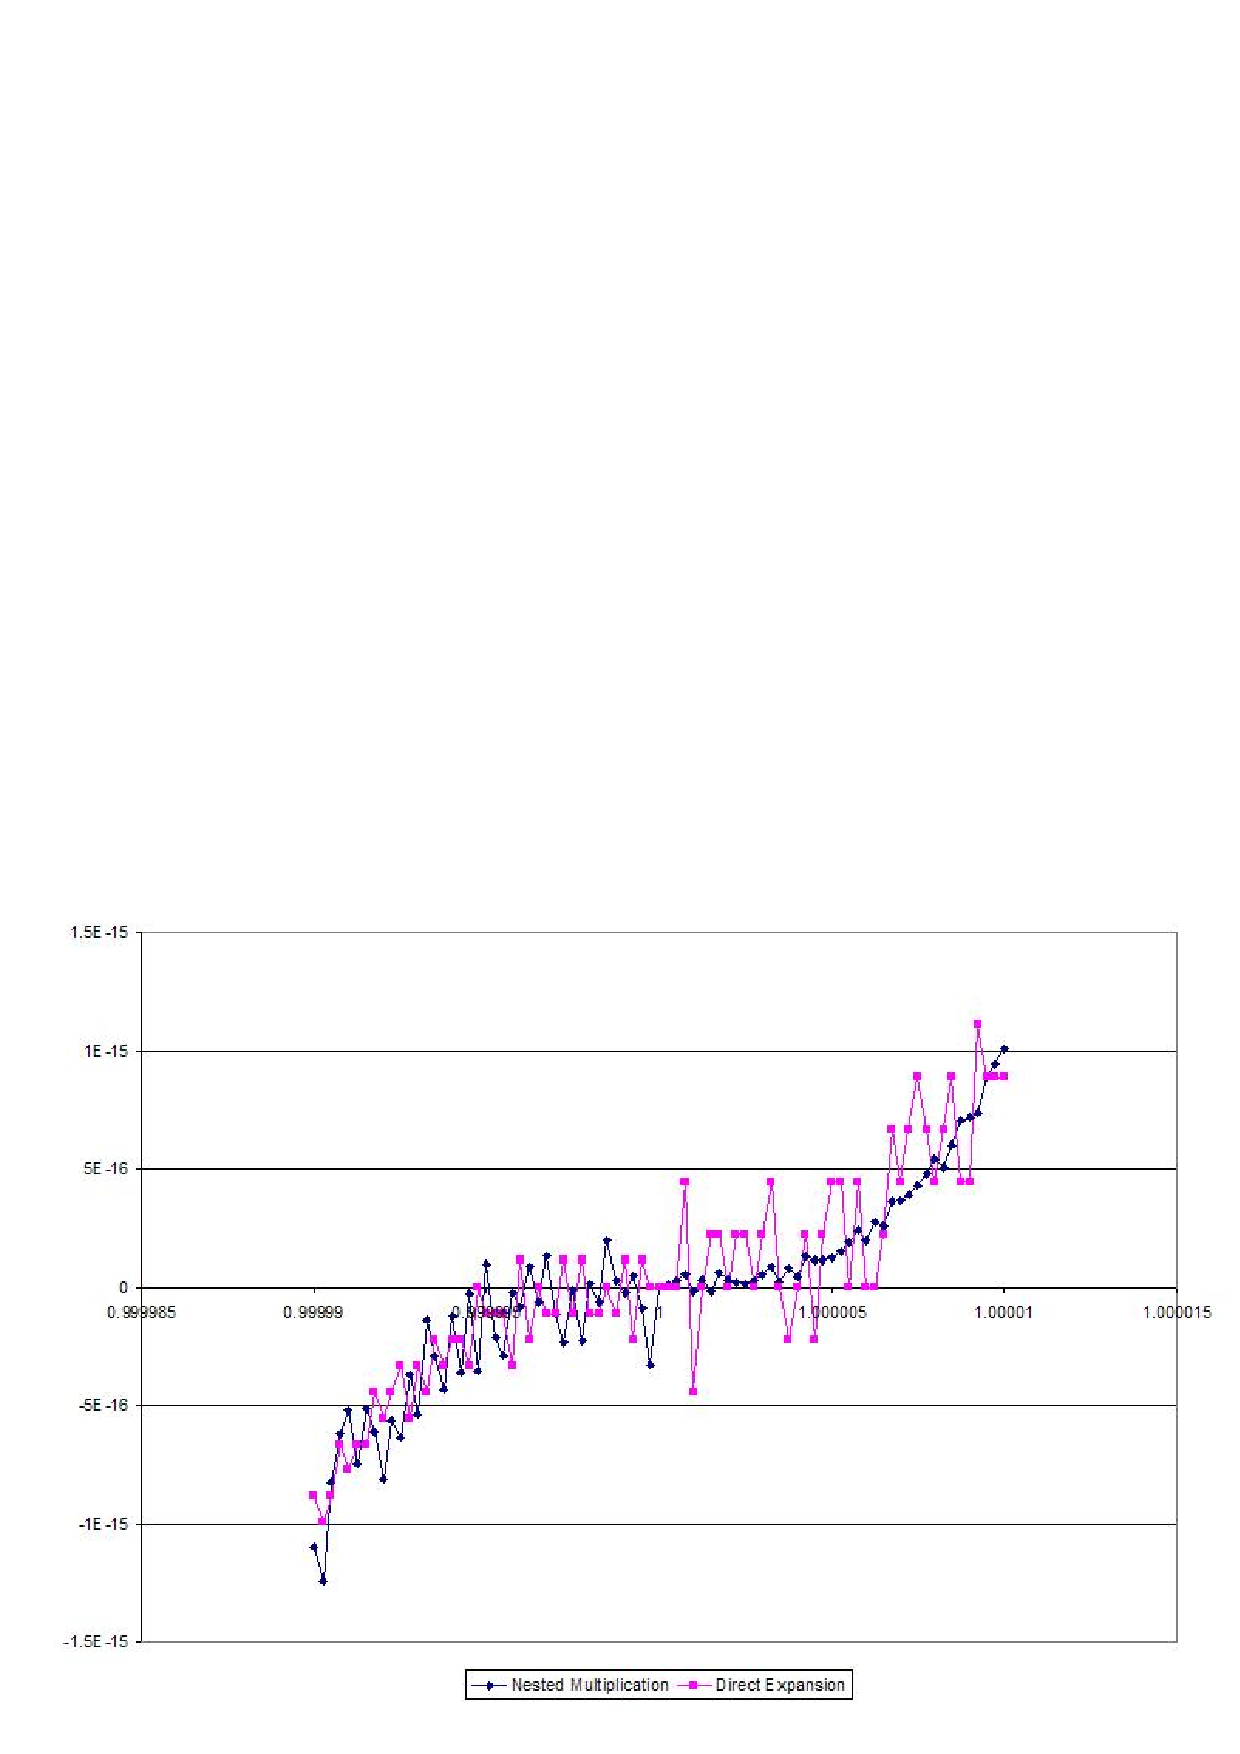
\includegraphics[width=4in]{cubicpoly.png}\\
  \caption{Close-up Look at Resulting Values of Two Evaluation Methods for $y=x^3-3x^2+3x-1$}\label{f-polyeval}
\end{figure}

\part{Organization}
\chapter{Arithmetic Operations}
\label{c-arith}


We have looked at number representation and calculation techniques, now we will look at how to specify the operations to a computer.  In order to do an arithmetic operation, we need to know where the two operands (sources) are located and where the result should be placed (destination).  Computers are classified by how many of the addresses must be explicitly stated and how many are implicit.

\section{Three Address Machines}

This is the most flexible form.  Each address can be specified by the user.  The commands are of the form

\begin{tabular}{c}
command source1, source2, destination \\
\textbf{or} \\
command destination, source1, source2 \\
\end{tabular}

\ThreeAddy

\section{Two Address Machines}

The destination is also a source in this case.  The commands are of the form

\begin{tabular}{c}
command destination, source \\
\end{tabular}

\section{One Address Machines}

A special register, called the accumulator, is designated to be a source and destination.  The accumulator has two special instructions, load accumulator and store accumulator.  Accumulator machines rarely use additional registers, though it is not technically required.  The arithmetic commands are of the form

\begin{tabular}{c}
command source \\
\end{tabular}

\section{Zero Address Machines}

The internal registers are arranged as a stack.  The source operands are taken from the stack in order (first operand on top, second operand below).  The result is pushed on the stack.  These are often called stack machines.  The arithmetic commands are of the form

\begin{tabular}{c}
command \\
\end{tabular}

\section{Comparison Code}

Consider the following equation:

\beqn
y & = & x^2+2x+3 \\
& = & (x+2)*x+3
\eeqn

Assume $x$ is at $100$, $2$ is at $104$, $3$ is at $108$, and $y$
is at $112$.  The following uses a three address scheme with destination first.

\vspace{.1in}
\begin{tabular}{ll} \hline
  % after \\ : \hline or \cline{col1-col2} \cline{col3-col4} ...
  version 1 & version 2 \\
  $y = x^2+2x+3$ & $y = (x+2)*x+3$ \\ \hline
  mpy 112,100,100 & add 112,100,104 \\
  mpy 116,100,104 & mpy 112,112,100 \\
  add 112,112,116 & add 112,112,108 \\
  add 112,112,108 &  \\ \hline
\end{tabular}
\vspace{.1in}

\vspace{.2in}
The following shows the second version on different machines.
\vspace{.1in}

\begin{tabular}{llll} \hline
  % after \\ : \hline or \cline{col1-col2} \cline{col3-col4} ...
  3 address       & 2 address    & 1 address & 0 address \\ \hline
  add 112,100,104 & move 112,100 & load 100  & push 100 \\
  mpy 112,112,100 & add 112,104  & add 104   & push 104 \\
  add 112,112,108 & mpy 112,100  & mpy 100   & add \\
                  & add 112,108  & add 108   & push 100 \\
                  &              & store 112 & mpy \\
                  &              &           & push 108 \\
                  &              &           & add \\
                  &              &           & pop 112 \\ \hline
\end{tabular}
\vspace{.1in}


Assume $x$ is in $R_1$, $2$ is in $R_2$, $3$ is in $R_3$, and $y$
is in $R_4$. 
\chapter{Stack Machines}
\label{c-stack}


Stack machines are also known as 0-address machines, because no address must be specified for arithmetic operations.  The most common example of a stack machine is an HP calculator.  The application "Toy Stack" is an executable for Windows XP, which is available at the website.  It has 64 bytes of memory split into 32 for instructions and 32 for data.  All variables are 1 byte long and stored in 2's complement or unsigned form.  Instructions are 1 byte long, but can have two commands in it in some cases.  There is no branch delay slot.  The commands are

\textbf{Memory}

\begin{tabular}{|cc|c|c|}
\hline
  0 & 0 & P & Addr \\ \hline
\end{tabular}

where,
\begin{eqnarray*}
  P &=& \left\{%
\begin{array}{ll}
    0, & \hbox{Push;} \\
    1, & \hbox{Pop.} \\
\end{array}%
\right.     \\
  Addr &=& \hbox{5-bit address in memory.}
\end{eqnarray*}


\textbf{Branching}

\begin{tabular}{|cc|c|c|}
\hline
  0 & 1 & C & Addr \\ \hline
\end{tabular}

where,
\begin{eqnarray*}
  C &=& \left\{%
\begin{array}{ll}
    0, & \hbox{Always;} \\
    1, & \hbox{Less (i.e. the top number on the stack is negative).} \\
\end{array}%
\right.     \\
  Addr &=& \hbox{5-bit address in memory to branch to.}
\end{eqnarray*}
Note: branch less is also branch bit set, for the most significant bit on the top of the stack.


\textbf{Arithmetic}

\begin{tabular}{|cc|c|c|}
\hline
  1 & 0 & $Op_1$ & $Op_2$ \\ \hline
\end{tabular}

where,
\begin{eqnarray*}
  Op_i &=& \left\{%
\begin{array}{ll}
    000, & \hbox{halt ($Op_1$) or nop ($Op_2$);} \\
    001, & \hbox{addition;} \\
    010, & \hbox{subtraction;} \\
    011, & \hbox{negation;} \\
    100, & \hbox{unsigned multiplication;} \\
    101, & \hbox{signed multiplication;} \\
    110, & \hbox{unsigned division;} \\
    111, & \hbox{signed division.} \\
\end{array}%
\right.
\end{eqnarray*}
Note: Nop is no operation, and is used to allow, just one arithmetic command to execute rather than two.  Halt is used to terminate the program run.  If something other than nop is in $Op_2$ after a halt then that command is executed before termination.


\textbf{Shifting}

\begin{tabular}{|cc|c|c|c|c|}
\hline
  1 & 1 & 0 & L/R & mode & times \\ \hline
\end{tabular}

where,
\begin{eqnarray*}
  L/R &=& \left\{%
\begin{array}{ll}
    0, & \hbox{left shift;} \\
    1, & \hbox{right shift.} \\
\end{array}%
\right. \\
  mode &=& \left\{%
\begin{array}{ll}
    00, & \hbox{fill with 0's;} \\
    01, & \hbox{fill with 1's;} \\
    10, & \hbox{arithmetic shift;} \\
    11, & \hbox{circulant shift.} \\
\end{array}%
\right. \\
times &=& \hbox{shift (1+times) bits (times is a two bit number).}
\end{eqnarray*}


\textbf{Push Signed Constant}

\begin{tabular}{|cc|c|c|c|}
\hline
  1 & 1 & 1 & 0 & Const \\ \hline
\end{tabular}

where, Const is a four bit number that is sign extended to eight bits and pushed on the stack.


\textbf{Logic}

\begin{tabular}{|cc|c|c|c|c|}
\hline
  1 & 1 & 1 & 1 & 0 & Op \\ \hline
\end{tabular}

where,
\begin{eqnarray*}
  Op &=& \left\{%
\begin{array}{ll}
    000, & \hbox{or;} \\
    001, & \hbox{nor;} \\
    010, & \hbox{orn;} \\
    011, & \hbox{xor;} \\
    100, & \hbox{and;} \\
    101, & \hbox{nand;} \\
    110, & \hbox{andn;} \\
    111, & \hbox{equivalence.} \\
\end{array}%
\right.
\end{eqnarray*}
Note: all logic functions are bitwise.


\textbf{Undefined}

\begin{tabular}{|cc|c|c|c|c|}
\hline
  1 & 1 & 1 & 1 & 1 & Op \\ \hline
\end{tabular}

where, Op is a three bit operand.  This operation is left undefined.

At the moment you have to enter your programs and data values manually, sorry I just started writing this.  A load and save feature has been added which saves the memory to a file in encrypted format.  You can only load programs that were encrypted with your exact name (spelling and caps count).  Essentially this removes sharing data files as you need to submit your solutions electronically to me, with the exact spelling of your name (so I can load them).  I will not give credit to you unless the name is yours.

\section{Affine Encryption Program}\label{s-stack-affine}

Affine encryption is one of the simplest methods for doing encryption.  Let $P_i$ be the $i^{th}$ character in the plain text message, and let $C_i$ be the corresponding encoded character.  Let there be $n$ possible characters to encode, then the basic idea is to pick two numbers $(a,b)$ to encode a message such that $\gcd(a,n)=1$ (so $a$ has an inverse).  No requirement on $b$ is needed if your modulus function has been encoded correctly.  The encoded character can then be found by
\begin{eqnarray*}
  a\times P_i +b &=& C_i \mod n.
\end{eqnarray*}
Note that the "$\mod n$" at the end says the equation holds in $\Zed_n$, the set of integers mod $n$ with appropriately defined arithmetic.

To decrypt the message, the equation
\begin{eqnarray*}
  \bar a\times (C_i +d) &=& P_i \mod n
\end{eqnarray*}
is used.  The term $\bar a$ is the inverse of $a$ in $\Zed_n$, which is found by solving
\begin{eqnarray*}
  a\times\bar a &=& 1 \mod n \\
   & \textbf{or} & \\
  a\times\bar a &=& m\times n+1.
\end{eqnarray*}
Note that $m$ is any whole number.  The term $d$ is the additive inverse of $b$ in $\Zed_n$, which is found by solving
\begin{eqnarray*}
  d=n-(b \mod n).
\end{eqnarray*}

We can summarize this by saying an affine cipher is an encryption technique that encodes using three integers: $a$, $b$, and $n$.  If $plain$ is the character to be encoded (with `A'=0 and `Z'=25) then $code=(a*plain+b) \mod n$.  Decoding is also done using three integers: $c$, $d$, and $n$.  If $code$ is the character to be encoded (with `A'=0 and `Z'=25) then $plain=(c*(code+d)) \mod n$.  The requirements on $(a,b,c,d,n)$ are:
\begin{itemize}
    \item $\gcd(a,n)=1$
    \item $(ac) \mod n = 1$
    \item $(b+d) \mod n = 0$
\end{itemize}
Below is C code to implement a particular case of affine cyphers.
\begin{verbatim}

char affine_encode(char plain){
    // affine codes capital letter in plain using a=5, b=12 thus this is modulo 26
    int iCode, iPlain, a=3,b=0;

    // convert char to integer and shift so A=0
    iPlain=int(plain)-65;

    // do the encoding
    iCode = (a*iPlain+b)%26;

    // return the result as a char
    return char(iCode+65);
}

char affine_decode(char code){
    // affine decodes capital letter in plain using c=21, d=8 thus this is modulo 26
    int iCode, iPlain, c=9, d=0;

    // convert char to integer and shift so A=0
    iCode=int(code)-65;

    // do the decoding
    iPlain = (c*(iCode+d))%26;

    // return the result as a char
    return char(iPlain+65);
}
\end{verbatim}


Using this we consider affine encryption for standard ASCII including the control codes.  In this case $n=2^7=128$.  Note that the standard arithmetic on our stack machine is $\Zed_{2^8}$ so we can calculate normally then drop the leading bit to get $\Zed_{2^7}$.  As long as $a$ does not have $2$ as a factor it will meet the requirement $\gcd(a,n)=1$.  Let $a=3$ then $3\times\bar a = m\times n+1$ for some $m\in\{1,2,\ldots\}$.  Start with $m=1$, then $\bar a = 129/3 = 43$.  Since the result is an integer, it is an inverse.  If the result was not an integer, $m$ would be incremented and the process would continue.  Finally, let $b=57$ then $d=128-57=71$.

Let the memory locations of the variables be:

\noindent\begin{tabular}{|c|c|c|}
  \hline
  Variable & Address & Value \\ \hline
  $P$      & 00000 & your choice \\ \hline
  $C$      & 00001 & per calculation \\ \hline
  $P$(calc)& 10000 & per calculation \\ \hline
  $a$      & 11100 & 00000011 \\ \hline
  $\bar a$ & 11101 & 00101011 \\ \hline
  $b$      & 11110 & 00111001 \\ \hline
  $d$      & 11111 & 01000111 \\ \hline
\end{tabular}

The variable $P$(calc) was added so the decoded plain text would not overwrite the original.  The program to encode is thus:

\begin{tabular}{l|l@{ ;}l}
  Machine & Assembly & Comment \\
  \hline
  00011110 & push $b$ & load data \\
  00011100 & push $a$ &  \\
  00000000 & push $P$ &  \\
           & unsigned multiply & aP+b \\
  10100001 & add      &  \\
  11000000 & shl0 1   & drop leading bit \\
  11010000 & shr0 1   &  \\
  00100001 & pop $C$  & store \\
  10000000 & halt     & done \\
\end{tabular}

The program to decode is thus:

\begin{tabular}{l|l@{ ;}l}
  Machine & Assembly & Comment \\
  \hline
  00011101 & push $\bar a$     & load data \\
  00011111 & push $d$          &  \\
  00000001 & push $C$          &  \\
           & add               & $\bar a(C+d)$ \\
  10001100 & unsigned multiply &  \\
  11000000 & shl0 1            & drop leading bit \\
  11010000 & shr0 1            &  \\
  00110000 & pop $P$(calc)     & store \\
  10000000 & halt              & done \\
\end{tabular}


\section{Babylonian Algorithm}

Implement the following Babylonian algorithm to find Pythagorean Triples\footnote{The algorithm actually predates Pythagoras.} on the Toy Stack.
\begin{itemize}
    \item Start with 2 (unsigned) integers $p$, $q$ with $p>q$ (assume these are present)
    \item calculate the three numbers by: $n_1=2pq$, $n_2=p^2-q^2$, $n_3=p^2+q^2$
\end{itemize}
To understand how this works note that
\beqn
n_1^2
&=&(2pq)^2 \\
&=&4p^2q^2
\eeqn
and
\beqn
n_2^2
&=&(p^2-q^2)^2 \\
&=&p^4-2p^2q^2+q^4
\eeqn
and
\beqn
n_3^2
&=&(p^2+q^2)^2 \\
&=&p^4+2p^2q^2+q^4
\eeqn
thus
\beqn
n_1^2+n_2^2
&=& (4p^2q^2)+(p^4-2p^2q^2+q^4) \\
&=& p^4+2p^2q^2+q^4 \\
&=& n_3^2
\eeqn
    {\color{ans}
    The assembly is

    \begin{verbatim}
    push 0   ! calculate 2pq
    push 1
    push #2
    umul
    umul
    pop 16   ! 2pq stored in 16
    push 0   ! calculate p^2
    push 0
    umul
    pop 2    ! p^2 stored in 2
    push 1   ! calculate q^2
    push 1
    umul
    pop 3    ! q^2 stored in 3
    push 3   ! calculate p^2 - q^2
    push 2
    sub
    pop      ! p^2 - q^2 stored in 17
    push 3   ! calculate p^2 + q^2
    push 2
    add
    pop      ! p^2 + q^2 stored in 17
    \end{verbatim}


    For the machine code see the website.
    } 
\chapter{Instruction Set Architecture}
\label{c-isa}

\section{RISC vs. CISC}

\ben
\item[RISC] reduced instruction set computer- For high level language programmers (reduces time for each instruction)
\item[CISC] complex instruction set computer- For assembly programmers (reduces instructions for same program)
\een

\vspace{.2in}
\noindent
\begin{tabular}{lp{2in}p{2in}}
                               & RISC  & CISC  \\
Number of addressing modes     & few   & many  \\
Access to main memory          & Only in loads and stores (hence load-store architecture) 
                                       & One or more operands in most instructions can access \\
Size of instruction set        & small & large \\
Complexity of each instruction & small & large \\
\end{tabular}
\vspace{.2in}

RISC is currently and has been more efficient.


\section{Memory Access}

Most machines are byte addressable (i.e. each byte in memory has an address).  Memory access typically come in three sizes and are often distinguished by the operand suffix .b (byte), .h (halfword), .w (word).  

\section{Branching}

Conditional branching

Three ways: compare two, compare to zero, condition registers

cmp

Branch delay and pipelining

short circuit (positional) put in sum of expressions form and then
do a series of conditional branches

Bitwise (and,or,xor,andn,orn)

bb (bitbranch reg,bit,targ)

bset

bclr

shift L/R

zero fill

one fill

rotate

usually to carry

\chapter{Addressing}
\label{c-address}


\begin{itemize}
  \item .bss
  \item .data
  \item .text
\end{itemize}

\begin{description}
  \item[.bss]  (block started by symbol) memory, reserved only
  \item[.data] memory, predefined values
  \item[.text] instructions
  \item[.reserve val] (alternately ".skip val") sets aside val bytes of memory
  \item[.equate name, val] (alternately ".set name, val") makes name a constant with value val
  \item[.byte val] (alternately .b, ub, sb) specifies the operation to be on a byte
  \item[.half val] (alternately .h, uh, sh) specifies the operation to be on a half word (2 bytes)
  \item[.word val] (alternately .w) specifies the operation to be on a word (4 bytes)
  \item[.align val] aligns the memory location counter
\end{description}

Note that val may be a constant expression for readability.

\noindent
\begin{tabular}{llll}
Name & Generic & Sparc & Uses \\ \hline
memory direct & mX & [\%r0+X] & \\
register direct & rX & \%rX & \\
immediate & \#X & X & \\
memory indirect & @mX & - & pointers \\
register indirect & @rX & [\%rX] & pointers \\
memory indexed & label[mX] & - & arrays \\
register indexed & label[rX] & [\%rY + \%rX] & arrays \\
 & & & (note \%rY is loaded with label) \\
pre-increment & +[rX] & - & increments by size (stride) each time \\
post-increment & [rX]+ & - & increments by size (stride) each time \\
pre-decrement & -[rX] & - & decrements by size (stride) each time \\
post-decrement & [rX]- & - & decrements by size (stride) each time \\
memory displaced & mX $\rightarrow$ label & - & struct \\
register displaced & rX $\rightarrow$ label & [\%rX + label] & struct \\
\end{tabular}


\begin{tabular}{cc}
\begin{tabular}{r|l|l|l|l|} \cline{2-5}
  m0  & 0x00 & 0x00 & 0x00 & 0x12 \\ \cline{2-5}
  m4  & 0x00 & 0x00 & 0x00 & 0x08 \\ \cline{2-5}
  m8  & 0x01 & 0x23 & 0x45 & 0x67 \\ \cline{2-5}
  m12 & 0x89 & 0xAB & 0xCD & 0xEF \\ \cline{2-5}
  m16 & 0x12 & 0x34 & 0x56 & 0x78 \\ \cline{2-5}
  m20 & 0x9A & 0xBC & 0xDE & 0xF0 \\ \cline{2-5}
  m24 & 0x11 & 0x11 & 0x11 & 0x11 \\ \cline{2-5}
\end{tabular}

&

\begin{tabular}{r|l|l|l|l|} \cline{2-5}
  r0  & 0x00 & 0x00 & 0x00 & 0x00 \\ \cline{2-5}
  r1  & 0x00 & 0x00 & 0x00 & 0x08 \\ \cline{2-5}
  r2  & 0x00 & 0x00 & 0x00 & 0x0C \\ \cline{2-5}
  r3  & 0x00 & 0x00 & 0x00 & 0x04 \\ \cline{2-5}
  r4  & 0x00 & 0x00 & 0x00 & 0x10 \\ \cline{2-5}
\end{tabular}
\end{tabular}
\vspace{.1in}

Let var1 be a label for the value 8.

\vspace{.1in}
\begin{tabular}{llll}
Representation & X=4 & Effective Address & Expression \\ \hline
mX & m4 & 0x00000004 & 0x00000008 \\
rX & r4 & - & 0x00000010 \\
\#X & \#4 & - & 0x00000004 \\
@mX & @m4 & 0x00000008 & 0x01234567 \\
@rX & @r4 & 0x00000010 & 0x12345678 \\
var1[mX] & 8[m4] & 0x00000010 (i.e.: 8+8) & 0x12345678 \\
var1[rX] & 8[r4] & 0x00000018 (i.e.: 8+16) & 0x11111111 \\
+[rX] & +[r4] & 0x00000014 & 0x9ABCDEF0 \\
      &       &  & r4 $\leftarrow$ 0x00000014 before \\
$[$rX]+ & [r4]+ & 0x00000010 & 0x12345678 \\
      &       &  & r4 $\leftarrow$ 0x00000014 after \\
-[rX] & -[r4] & 0x0000000C & 0x89ABCDEF \\
      &       &  & r4 $\leftarrow$ 0x0000000C before \\
$[$rX]- & [r4]- & 0x00000010 & 0x12345678 \\
      &       &  & r4 $\leftarrow$ 0x0000000C after \\
mX $\rightarrow$ var1 & m4 $\rightarrow$ 8 & 0x00000010 (i.e.: 8+8) & 0x12345678 \\
rX $\rightarrow$ var1 & r4 $\rightarrow$ 8 & 0x00000018 (i.e.: 8+16) & 0x11111111 \\
\end{tabular}


\subsection{Arrays}

For instance consider an array of 10 integers.

\begin{verbatim}
   int my_int[10];
\end{verbatim}

This creates both the array of integers and a pointer to the first element.  The elements are numbered 0 to 9 and are accessed by $my_int[i]$ for $i\in\{0,1,\ldots,9\}$.  They can also be accessed by $*(my_int+i)$.  In assembly we would have:

\begin{verbatim}
  my_int:  .skip 10*4    ; each int is 4 bytes
\end{verbatim}

The contents can be accessed by:

\begin{verbatim}
  set i, %r2
  ld  [%r2], %r2
  umul %r2, 4, %r3
  set my_int, %r4

  ld [%r4 + %r3], %r5
\end{verbatim}

or if my\_int (the address) fits in a 13 bit signed constant:

\begin{verbatim}
  set i, %r2
  ld  [%r2], %r2
  umul %r2, 4, %r3

  ld [%r3+my_int], %r5
\end{verbatim}

Essentially the address is my\_int + i*4, but this assumes that start of my array is zero.  How about a language like Pascal or VB which allows other starting values?  Consider defining an array (-m,-m+1,\ldots, -1, 0, 1, \ldots, n).  To use the address my\_int + i*size we have

\begin{verbatim}
          .skip m*size       ! negatives
          .skip (n+1)*size   ! zero and positives
\end{verbatim}

Alternately,

\begin{verbatim}
         .skip (m+n+1)*size  ! whole thing
\end{verbatim}

This causes the address to be my\_int + (i+m)*size.  Now you might think this will be longer, but note that it can be rewritten as

\vspace{.1in}
\begin{tabular}{l}
    my\_int + (i+m)*size \\
    my\_int + i*size + m*size \\
    (my\_int + m*size) + i*size \\
\end{tabular}
\vspace{.1in}

That is, rather than constantly biasing the index, it makes more sense to bias the base.  Essentially it makes the second method look like the first, but it works for a positive starting number (by making m a negative).  Since it is more general the later form is what is used in practice.

\subsection{String Storage}

\begin{description}
  \item[string256] (aka length plus value) length of string in first byte, string following
  \item[NULL terminated] string followed by 0
\end{description}


\subsection{Structs}

\begin{verbatim}
struct book{
  int pages;
  float price;
  char title[20];
}library[100];
\end{verbatim}

Would be implemented:

\begin{verbatim}
         .set pages, 0
         .set price, 4
         .set title, 8
         .set book_size, 28

.bss

library: .skip 100*book_size
\end{verbatim}

.bss is done in .data on some assemblers or machines 
\chapter{Subroutines}
\label{c-subs}


\section{Basic Overview}

Before we get into this, let's establish some basic definitions.

\begin{description}
  \item[Caller] the section of code that initiates the call
  \item[Callee] the section of code that is called
  \item[Return Address] The address of the instruction to be
  executed after the call is done (usually the one following the
  branch or jump)
  \item[Subroutine Linkage]   data structure used to share information between
  caller and callee
\end{description}

\subsection{What needs to be passed?}

A subroutine can be called from different sections of code and with different parameters.  The subroutine needs to know what data it must operate on and where to resume execution when it finishes.  Additionally the subroutine usually must return some data, and thus it must place the data in an easy to locate area.  The basic data that must be exchanged is thus,

\begin{itemize}
    \item return address
    \item return value
    \item parameters
\end{itemize}

\subsection{General Call Sequence}

\begin{tabular}{|c|c|c|}
  \multicolumn{1}{c}{Caller} & \multicolumn{1}{c}{ } & \multicolumn{1}{c}{Callee} \\
  & & \\
  \cline{1-1} \cline{3-3}
  Startup  & $\rightarrow$ & Prologue \\ \cline{3-3}
  Sequence &   & Body \\ \cline{1-1}
  Cleanup  &   & Body \\ \cline{3-3}
  Sequence & $\leftarrow$ & Epilogue \\ \cline{1-1} \cline{3-3}
  & & \\
\end{tabular}

\section{Return Addresses in Leaf and Non-Leaf Subroutines}

For the moment we will look only at the issues surrounding return addresses.  The following distinctions must be made:
\begin{quote}
Leaf subroutines do not make subroutine calls, where as non-leaf subroutines call at least one subroutine (itself or another subroutine).
\end{quote}


The most basic leaf subroutine call looks like:

\begin{tabular}{|c|c|c|}
  \multicolumn{1}{c}{Caller} & \multicolumn{1}{c}{ } & \multicolumn{1}{c}{Callee} \\
  & & \\
  \cline{1-1} \cline{3-3}
  address+(4 or 8) to r31  & $\rightarrow$ & none \\ \cline{3-3}
  branch sub     &   & Body \\ \cline{1-1}
  none           &   & Body \\ \cline{3-3}
  none           & $\leftarrow$ & branch @r31 \\ \cline{1-1} \cline{3-3}
  & & \\
\end{tabular}

The basic leaf routine is quick and easy, but it cannot be used on non-leaf procedures as the return address would be lost.  Consider the following subroutine to calculate $x^n$:

\noindent
\begin{tabular}{p{3.4in}|p{2.7in}}
Code & Sample run \\ \hline
\begin{verbatim}
!!!!!!!!!!!!!!!!!!!!!!!!!!!!!!!!!!!!!!!!!!!!
!! name: pow
!! desc: calculates x^n
!! meth: recursive function call
!!            x*(x^{n-1})
!! parm: x in r8
!!       n in r9
!! pre : nothing in r16, it is used as
!!       a temporary variable
!! post:
!! ret : x^n in r8
!! date: 20 May 2003
!! rev : 1.0
!! revh:
!!!!!!!!!!!!!!!!!!!!!!!!!!!!!!!!!!!!!!!!!!!!
pow:        cmp r9,r0        ! see if x^0
            breq,a pow_done  !  if n=0
            add r0,1,r8      !  then ans=1

            cmp r9,1         ! see if x^1
            breq pow_done    ! if n=1
            nop              ! then ans=x

            mv r8,r16        ! else n>1
            call pow         ! calc r8=x^{n-1}
            sub r9,1,r9      !
pow_r:      smul r16,r8,r8   ! ans = x*x^{n-1}
pow_done:   retl
            nop
\end{verbatim}

&

Assume the call was to calculate $5^2$ and return to the label "retn".  For our machine the return address is stored in r31.  We will assume that annulled commands become nop's (they really do, the results are just sent to r0 and the condition codes are not set).

\begin{tabular}{lcccc}
  Instruction & r8 & r9 & r16 & r31 \\ \hline
  cmp r9,r0 & 5 & 2 & - & retn \\
  breq,a pow\_done & 5 & 2 & - & retn \\
  nop & 5 & 2 & - & retn \\
  cmp r9,1 & 5 & 2 & - & retn \\
  breq pow\_done & 5 & 2 & - & retn \\
  nop & 5 & 2 & - & retn \\
  mv r8,r16 & 5 & 2 & 5 & retn \\
  call pow & 5 & 2 & 5 & pow\_r \\
\end{tabular}

Notice at this point we lost the return address!

\begin{tabular}{lcccc}
  Instruction & r8 & r9 & r16 & r31 \\ \hline
  sub r9,1,r9 & 5 & 1 & 5 & pow\_r \\
  cmp r9,r0 & 5 & 1 & 5 & pow\_r \\
  breq,a pow\_done & 5 & 1 & 5 & pow\_r \\
  nop & 5 & 1 & 5 & pow\_r \\
  cmp r9,1 & 5 & 1 & 5 & pow\_r \\
  breq pow\_done & 5 & 1 & 5 & pow\_r \\
  nop & 5 & 1 & 5 & pow\_r \\
  retl & 5 & 1 & 5 & pow\_r \\
  nop & 5 & 1 & 5 & pow\_r \\
  smul r16,r8,r8 & 25 & 1 & 5 & pow\_r \\
  retl & 25 & 1 & 5 & pow\_r \\
  nop & 25 & 1 & 5 & pow\_r \\
\end{tabular}

At this point it should have gone back to "retn" but since that address was lost it will loop endlessly.

\\
\end{tabular}

If the subroutine is non-leaf and not part of a cycle (recursive or otherwise) then the following modification will work nicely.
\vspace{6pt}

\begin{tabular}{|c|c|c|}
  \multicolumn{1}{c}{Caller} & \multicolumn{1}{c}{ } & \multicolumn{1}{c}{Callee} \\
  & & \\
  \cline{1-1} \cline{3-3}
  address+(4 or 8) to r31  & $\rightarrow$ & r31 to mem \\ \cline{3-3}
  branch sub     &   & Body \\ \cline{1-1} \cline{3-3}
  none           &   & mem to r31 \\
  none           & $\leftarrow$ & branch @r31 \\ \cline{1-1} \cline{3-3}
  & & \\
\end{tabular}

\vspace{6pt}
the two versions can be combined as:
\vspace{6pt}

\begin{tabular}{|c|c|c|}
  \multicolumn{1}{c}{Caller} & \multicolumn{1}{c}{ } & \multicolumn{1}{c}{Callee} \\
  & & \\
  \cline{1-1} \cline{3-3}
  address+(4 or 8) to r31  & $\rightarrow$ & if nonleaf r31 to mem \\ \cline{3-3}
  branch sub     &   & Body \\ \cline{1-1} \cline{3-3}
  none           &   & if nonleaf mem to r31 \\
  none           & $\leftarrow$ & branch @r31 \\ \cline{1-1} \cline{3-3}
  & & \\
\end{tabular}

\section{Parameter Passing}

We now turn our attention on the parameters.  First we need to consider how to represent the data.  For instance if you just need to send an integer to do a calculation but you don't want it modified then you would pass by value.  If on the other hand you need to pass an instance of a class you must pass by reference.  The three ways data may be handled are

\begin{enumerate}
    \item pass by value (not returned)
    \item pass by value/result (modify and return)
    \item pass by ref (pointer to actual object)
\end{enumerate}

Beyond these basic considerations, there is a question as to where to locate the data for the subroutine call.  The information could be located in the registers for speed, or in static variables in RAM (parameter block).  Neither of the options discussed so far will handle cyclic subroutines or dynamic local variables.  If either cyclic subroutines or dynamic local variables are needed the information must be passed on the stack (dynamic variables in RAM).  The methods are:

\begin{enumerate}
    \item register
    \begin{itemize}
        \item fast
        \item leaf subroutine
    \end{itemize}
    \item parameter block
    \begin{itemize}
        \item larger data
        \item non-leaf and non-cyclic subroutines
    \end{itemize}

    \item stack
    \begin{itemize}
        \item larger data
        \item (dynamic) local variables
        \item cyclic and recursive calls
    \end{itemize}
\end{enumerate}

\section{Register}

\begin{tabular}{|c|c|c|}
  \multicolumn{1}{c}{Caller} & \multicolumn{1}{c}{ } & \multicolumn{1}{c}{Callee} \\
  & \multicolumn{1}{c}{ } & \multicolumn{1}{c}{} \\ \cline{1-1}
  mv params into r8 to r13 & & \\ \cline{3-3}
  address+(4 or 8) to r31  &  & none \\ \cline{3-3}
  branch sub     & $\nearrow$  & Body \\ \cline{1-1} \cline{3-3}
  none           &   & mv result to r8 \\
  none           & $\nwarrow$ & branch @r31 \\ \cline{1-1} \cline{3-3}
  & & \\
\end{tabular}



\vspace{6pt}
\textbf{Example}
\vspace{6pt}

We have discussed affine ciphers already.  You might have noticed that the equation for encoding and decoding is very similar.  We can combine them with only a small alteration to the decoding formula and one of the requirements.  Decoding is still done using three integers: $c$, $d$, and $n$.  If $code$ is the character to be decoded (with `A'=0 and `Z'=25) then $plain=(c*code+d) \mod n$.  The requirements on $(a,b,c,d,n)$ are:
\begin{itemize}
    \item $\gcd(a,n)=1$
    \item $(ac) \mod n = 1$
    \item $(cb+d) \mod n = 0$
\end{itemize}
Below is C code to implement a particular case of affine cyphers.
\begin{verbatim}

char affine(char letter, int scale, int offset){
    // affine codes capital letter in 'letter' thus this is modulo 26
    int iCode, iLetter;

    // convert char to integer and shift so A=0
    iLetter=int(plain)-65;

    // do the encoding
    iCode = (scale*iLetter+offset)%26;

    // return the result as a char
    return char(iCode+65);
}

\end{verbatim}

The SPARC syntax is then


    \textbf{affine}

    \begin{verbatim}
            ! calculates affine encryption:
            !    crypt = (a*(orig-off)+b) mod p + off
            ! a     is passed   in r8
            ! b     is passed   in r9
            ! n     is passed   in r10
            ! off   is passed   in r11
            ! orig  is passed   in r12
            ! crypt is returned in r
            .text
    affine: sub  r12, r12, r11  ! orig-off
            mult r8,  r12, r8   ! a*(orig-off)
            add  r8,  r8,  r9   ! a*(orig-off)+b
            div  r9,  r8,  r10  ! x= y mod z = y - y/z*z
            mult r9,  r9,  r10
            sub  r8,  r8,  r9   ! (a*(orig-off)+b) mod n
            add  r8,  r8,  r11  ! done
            retl
    \end{verbatim}


    \textbf{encrypt call}

    \begin{verbatim}
            ! affine encrypt
            ! a is passed in r8
            ! b is passed in r9
            ! n     is passed   in r10
            ! off   is passed   in r11
            ! orig  is passed   in r12
            ! crypt is returned in r8
            .text
            set r8, 3            ! given
            set r9, 0            ! given
            set r10, 26          ! letters in alphabet
            set r11, 65          ! A in ascii
            call affine          ! call and link
            ld.b r12, add_plain  ! assume have label add_plain
                                 !   where plain text is stored
            st.b r8,  add_code   ! assume have label add_code where
                                 !   cypher text is to be stored
    \end{verbatim}


    \textbf{decrypt call}

    \begin{verbatim}
            ! affine decrypt
            ! a is passed in r8
            ! b is passed in r9
            ! n     is passed   in r10
            ! off   is passed   in r11
            ! orig  is passed   in r12
            ! crypt is returned in r8
            .text
            set r8, 9            ! given
            set r9, 0            ! given
            set r10, 26          ! letters in alphabet
            set r11, 65          ! A in ascii
            call affine          ! call and link
            ld.b r12, add_code   ! assume have label add_code
                                 !   where cypher text is stored
            st.b r8,  add_plain  ! assume have label add_code where
                                 !   plain text is to be stored
    \end{verbatim}






\vspace{6pt}
\textbf{Example}
\vspace{6pt}


Write the MIPS assembly code for the following function.  Assume the array a has been defined as size \textbf{n}.  The following registers are to be used to pass the values:

    \begin{tabular}{ll}
    pointer to a  &  \verb $a0 \\
    n             &  \verb $a1 \\
    sum           &  \verb $v0 \\
    \end{tabular}

You do not need to write the code to call the function.

\begin{verbatim}
  int sum(int* a, int n){
    int sum;
    sum=0;
    for(int i=0;i<n;i++){
      sum+=a[i]}
    return sum;}
\end{verbatim}



\vspace{6pt}
\textbf{Solution}
\vspace{6pt}

\begin{verbatim}
  sum:
    add $v0, $zero, $zero   # sum=0
    sll $a1, $a1, 2         # 4*n
    add $a1, $a1, $a0       # one element after last in array
    ble $a1, $a0, sum_done  # array empty
  sum_loop:
    lw $t0, 0($a0)          # get element
    addi $a0, $a0, 4        # increment pointer
    add $v0, $v0, $t0       # add element to sum
    bne $a0, $a1, sum_loop  # check if more elements
  sum_done:
    jr $ra                  # return
\end{verbatim}



\section{Parameter Block}

\begin{tabular}{|c|c|c|}
  \multicolumn{1}{c}{Caller} & \multicolumn{1}{c}{ } & \multicolumn{1}{c}{Callee} \\
  &  &  \\ \cline{1-1} \cline{3-3}
  store params into block using labels & & allocate block and labels in .data \\
  store address+(4 or 8) to block  &  & none \\ \cline{3-3}
  branch sub     & $\nearrow$  & Body \\ \cline{1-1} \cline{3-3}
  load result to desired register &   & store result to block \\
  none           & $\nwarrow$ & ld return address to r31 \\
  none           &  & branch @r31 \\ \cline{1-1} \cline{3-3}
  & & \\
\end{tabular}

\section{Stack}

The stack is a large block of RAM which data is pushed onto.  Any piece of information can be pushed onto the stack.  All the data passed to and from the subroutine with all the local variables composes a block of information on the stack called the frame.  The frame is created in the startup and prologue and removed in the epilogue and cleanup.  The startup allocates space for all the information that must be passed (return address, parameters, and return values), and the cleanup removes it.  The prologue allocates any local variables or storage to protect registers and the epilogue removes this local information.

\begin{tabular}{|c|c|c|}
  \multicolumn{1}{c}{Caller} & \multicolumn{1}{c}{ } & \multicolumn{1}{c}{Callee} \\
   & \multicolumn{1}{c}{ } & \multicolumn{1}{c}{} \\ \cline{1-1}
  push params &  &  \\ \cline{3-3}
  allocate return value & & push registers to protect \\
  push return address  & $\nearrow$ & push local variables \\ \cline{3-3}
  branch sub     &   & Body \\ \cline{1-1} \cline{3-3}
  pop result to desired register &   & store result to stack at offset \\
  pop params   & $\nwarrow$ & pop locals (remove) \\
       &  & pop register back \\ \cline{1-1}
       &  & pop return address to r31 \\
       &  & branch @r31 \\ \cline{3-3}
  & & \\
\end{tabular}

\begin{verbatim}
!!!!!!!!!!!!!!!!!!!!!!!!!!!!!!!!!!!!!!!!!!!!
!! name: pow
!! desc: calculates x^n
!! meth: recursive function call
!!            x*(x^{n-1})
!! parm: stack passing:
!!       x              at fp+20
!!       n              at fp+16
!!       return value   at fp+12
!!       return address at fp+8
!! pre :
!! post:
!! ret : x^n at fp+12
!! date: 22 May 2003
!! rev : 1.1
!! revh:
!!!!!!!!!!!!!!!!!!!!!!!!!!!!!!!!!!!!!!!!!!!!
            .set s16,0       ! offset to save r16
            .set s17,4       ! offset to save r17
            .set ra,8        ! offset to ret add
            .set rv,12       ! offset to ret val
            .set n,16        ! offset to n
            .set x,20        ! offset to x
pow:        sub sp,8,sp      ! allocate save space
            mv sp,fp         ! set frame
            st r16,[fp+s16]  ! save r16
            st r17,[fp+s17]  ! save r17

            ld [fp+n],r17    ! load n
            cmp r17,r0       ! see if x^0
            breq,a pow_done  !  if n=0
            add r0,1,r16     !  then ans=1

            cmp r17,1        ! see if x^1
            breq pow_done    !  if n=1
            ld [fp+x],r16    !  then ans=x

                             ! else n>1
            sub sp,4,sp      !  decrement pointer
            st r16,[sp]      !  push x
            sub r17,1,r17    !  calc n-1
            sub sp,4,sp      !  decrement pointer
            st r17,[sp]      !  push n-1
            sub sp,8,sp      !  decrement pointer
                             !  for return value
                             !  and address
            call pow         !  calc r8=x^{n-1}
            st r31,[sp]      !  push return address

            ld [sp],r16      !  get x^{n-1}
            add sp,12,sp     !  deallocate
            mv sp,fp         !  restore frame

            ld [fp+x],r17    !  get x
            smul r16,r17,r16 !  ans = x*x^{n-1}

pow_done:   st r16,[fp+rv]   ! store return value
            ld [fp+s16],r16  ! restore r16
            ld [fp+s17],r17  ! restore r17
            ld [fp+ra],r31   ! get return address
            retl
            add sp,12,sp     !  deallocate ra, s16, s17
\end{verbatim}


\section{Temperature Conversion}

Write a function that converts Fahrenheit to Celsius by following the steps below.  A C/C++ command to do the conversion is:
    \begin{verbatim}

    celsius = ((fahrenheit - 32)* 5) / 9;
    \end{verbatim}
    Note: I added an extra set of parenthesis to let you know you must do the multiplication first!  Why does the multiplication have to be done first?  Include an example.

    {\color{ans}
        If you do not multiply first, you can loose precision.  ex: 2/9*5=0, while 2*5/9=1 (in integer math).
    }

    \begin{enumerate}
        \item State the passing convention you will use (include what needs to be passed and where you will pass it) and any other reasonable assumptions on the machine.

        {\color{ans}
        I will use register passing and will use register r8 to pass both the parameter and the result.  Since this is a leaf procedure and I do not need other registers, I will use the book's leaf procedure (return address in r31).  I will further assume that my machine has call and retl that automatically store and access the return address.  Finally, I will assume there is a branch delay slot, the destination is always the first location, and I have all addressing modes.  (your choices may be different).
        }

        \item Write the function.

        {\color{ans}
        \begin{verbatim}
        fahr_2_cels:   sub r8, r8, 32
                       mpy r8, r8, 5
                       retl
                       div r8, r8, 9
        \end{verbatim}

        }

        \item Show how it would be called.  Assume that the Fahrenheit temperature is stored in a memory location specified by the label "fahr\_temp".  The result should be stored at the memory location specified by the label "cels\_temp".

        {\color{ans}
        \begin{verbatim}
                       set r1, fahr_temp
                       call fahr_2_cels
                       ld.w r8, @r1
                       set r1, cels_temp
                       st.w @r1, r8
        \end{verbatim}

        }

    \end{enumerate}

\input{Kohw_mips}
\chapter{Data Transfer}
\label{c-comps}


\section{I/O}

Transmission of data from one device to another is the essence of
I/O.  Usually, I/O is accomplished by defining registers to hold
the information necessary to transmit the data.  The registers
that handle the transmission are called the I/O port. At least
three registers are used, one for the data, one for the control,
and one for the Status.
\begin{description}
  \item[Data] the codes to be transmitted.  These can be
  traditional codes, such as ASCII, or even an address of data
  being requested.
  \item[Control] the commands specifying what is to be done.
  \item[Status] a series of bits specifying what is going on with
  the bus and the current transaction.
\end{description}
Accessing the registers (reading from or writing to) can be
accomplished in two ways.
\begin{description}
  \item[Memory Mapped] the registers of the I/O port, have
  addresses in regular memory, and thus can be treated as a
  regular memory location for access purposes.
  \item[Isolated] the registers are in a separate (isolated)
  memory address scheme, and thus the memory must be access
  through special commands.
\end{description}


\section{Busses} \label{s-busses}

Internal vs. External (relative to cpu)

Master/Slave (initiator/target)

\begin{description}
  \item[(Transaction) Master] the initiator of a transaction.
  \item[(Transaction) Slave] the target of a transaction.
  \item[Bus Master] any device that can be a (transaction) master.
  \item[Burst Mode Transaction] transaction which transmits several
  values.
  \item[Bus Transaction] data transfer on an external bus.
\end{description}
Synchronous Bus Lines

\begin{tabular}{lcl}
  Line/Signal        & Num & Owner        \\ \hline
  Clock              & 1   & Bus          \\
  Start              & 1   & Master       \\
  Address            & k   & Master       \\
  $R$/$\overline{W}$ & 1   & Master       \\
  Data               & n   & Master/Slave \\
  Done               & 1   & Slave        \\
\end{tabular}

Arbitration is usually overlapped

\subsection{Synchronous/Asynchronous Transfer}

Busses have to have a way to specify when to transfer and if data
has been received.  The two basic schemes for transfer is
synchronous and asynchronous.

Synchronous transfers uses a clock signal to coordinate
communication, and is thus very fast.  For a data request, we only
need to spend one bus cycle to sent the request, the access time to
find the data, and one bus cycle to send the answer.  The time to
transmit the data is thus
\beqn
T_{transmit}=\frac{2}{f_{bus}}+T_a,
\eeqn
were $T_a$ is the time to access the data, and $f_{bus}$ is the bus clock rate\footnote{A one way transmission must finish in this time.}.  The faster the clock the less time to transmit the data.  The bandwidth of the bus in terms of transactions is
\beqn
BW_{transaction}=\frac{W_{bus}}{T_{transmit}},
\eeqn
where $W_{bus}$ is the width of the bus\footnote{How much data can be sent simultaneously, i.e. the number of wires measured in bits or bytes.  A bus that has 32 data wires is 32 bits wide or 4 bytes wide.}.  Frequently however, buses are measured not by an actual transaction but by what a one way message would be
\beqn
BW &=& \frac{W_{bus}}{T_{bus}}\\
   &=& W_{bus}f_{bus}.
\eeqn
Let's consider a few examples.  Note that we will be reporting bandwidth in megabytes per second (MB/s).  A byte is 8 bits, and a megabyte is $2^{20}$ bytes.  Bus frequencies (sometimes called speeds) are reported in megaHertz (MHz), but here mega is in base 10 not base 2, so it is $10^6$ Hertz.  Recall a Hertz is a reciprocal second.  Sometimes this distinction is ignored to simplify calculations.

\begin{example}[PCI]
A basic PCI bus is 32 bits wide (4 bytes) and runs at 33.3 MHz.  Thus the bandwidth is
\begin{eqnarray}
BW 
&=& W_{bus}f_{bus} \\
&=& \left(4 [B]\frac{1 [MB]}{2^{20} [B]}\right)\left(33.3 [MHz]\frac{10^6 [Hz]}{1 [MHz]}\right) \\
&=& \left(\frac{1}{2^{18} [MB]}\right)\left(3.33\times 10^7 [Hz]\right) \\
&=& \left(\frac{1}{2^{18} [MB]}\right)\left(3.33\times 10^7 [Hz]\right) \\
&\approx & 127 [MB/s]
\end{eqnarray}
\end{example}



Clock signals take time to transfer down the wire and thus is subject to clock skew.  To understand clock skew, consider a simple example of two clocks 3 kilometers apart.  The clocks are synchronized by a beam of light, which travels at $3\times 10^5$ km/s, and thus it takes 10$\mu$s for the synchronization pulse to arrive from the master clock.  If the clocks were only synchronized once per second the fraction of the synchronization time used to transmit the pulse would be $\frac{10\mu s}{1s}=.001\%$, which is basically insignificant. What if we wanted to synchronize the clocks every tenth of a milisecond (.1ms)? The fraction of time to transfer now is $\frac{10\mu s}{.1ms}=10\%$, which is very significant.  When the clock pulse arrives it is off by 10\%!  That is called clock skew, when the transmission time of the clock pulse takes a significant portion of the clock frequency.  Clock skew is effected by the distance ($d$) and the clock rate ($f$).  If the clock skew is some fraction ($s$) and we assume that the clock signal is carried at the speed of light ($c$) then the relation between the variables is
\beqn
\frac{d}{c} = \frac{s}{f}
\eeqn
Assuming we want the skew to be less than a third ($s=.33\ldots$), the distance is measured in meters and the bus clock will be measured in megahertz, then
\beqn
df=100.
\eeqn
In other words a 100MHz bus (f=100) can only be 1 meter long (d=1) to keep clock skew under 33.3\%!  Given that bus speeds of 400MHz are very reasonable, this would limit bus length to about 9in.  Thus we see that clock skew limits bus length, and thus synchronous buses are fast but short.

Asynchronous transfers get around the problem of clock skew by doing a procedure called handshaking.  Basically two units that want to talk send messages back and forth letting each other know what is going on.  A basic handshaking protocol between a sender (S) and a receiver (R) to request data from R is
\begin{enumerate}
  \item S to R: Here is the address of the data I want.
  \item R to S: I got your request and will look it up.
  \item S: Drop request when recieve
  \item R: looking up data.
  \item R to S: Here is your data.
  \item S to R: I got it.
  \item S: Wait till see data signal drop then drop acknowledgement.
\end{enumerate}
Call the time for the signal to travel from sender to receiver or vice versa $T_h$ (for handshake time), and the time to get the data as $T_a$(for access time).  If we are clever we can overlap items 2,3 with item 4, so that we will only take the longer of $2T_h$ or $T_a$ rather than $2T_h+T_a$.  The total time for one transfer is thus
\beqn
T_{transfer}=4T_h+\max(2T_h,T_a).
\eeqn
The bandwidth of the bus is the rate at which data can be sent, and
thus
\beqn
BW &=& \frac{W_{bus}}{T_{transfer}},
\eeqn
where $W_{bus}$ is the width of the bus.

\subsection{Polling and Interrupts}

There are two basic ways to handle bus communication with the CPU:
polling, interrupts.  Direct Memory Access (DMA) is a special case
of interrupts.

\subsubsection{Polling - CPU Controlled Data Transfer}

\beqn
\hbox{Fraction of CPU Time}
&=& \frac{\hbox{Cycles Per Second used on Polls}}{\hbox{Clock Frequency}} \\
&=& \frac{\frac{\hbox{Polls}}{\hbox{Sec}}\frac{\hbox{Cycles}}{\hbox{Poll}}}{\hbox{Clock Frequency}} \\
&=& \frac{\frac{\hbox{Data Rate}}{\hbox{Poll Size}}\frac{\hbox{Cycles}}{\hbox{Poll}}}{\hbox{Clock Frequency}}
\eeqn


\subsubsection{Interrupt Driven - CPU Controlled Data Transfer}

\beqn
\hbox{Fraction of CPU Time}
&=& \frac{\hbox{Cycles Per Second used on Interrupts}}{\hbox{Clock Frequency}} \\
&=& \frac{\frac{\hbox{Interrupts}}{\hbox{Sec}}\frac{\hbox{Cycles}}{\hbox{Interrupts}}}{\hbox{Clock Frequency}} \\
&=& \frac{\frac{\hbox{Data Rate}}{\hbox{Packet Size}}\frac{\hbox{Cycles}}{\hbox{Interrupt}}}{\hbox{Clock Frequency}}
\eeqn


\subsubsection{Interrupt Driven - Direct Memory Access (DMA)}

\beqn
T_{\hbox{Transfer}}
&=&\frac{\hbox{Size Transfer}}{\hbox{Speed Transfer}} \\
&=&\frac{\hbox{Data Size}}{\hbox{Data Rate}} \\
\hbox{Cycles to Handle}
&=& C_h \\
&=&\frac{\hbox{Cycles to Start}+\hbox{Cycles to Complete}+f_e\times\hbox{Cycles to handle errors}}{1-f_e} \\
\hbox{Fraction of CPU Time}
&=& \frac{\hbox{Cycles Per Second used to handle DMA}}{\hbox{Clock Frequency}} \\
&=& \frac{\frac{C_h}{T_{\hbox{Transfer}}}}{\hbox{Clock Frequency}} \\
&=& \frac{C_h}{T_{\hbox{Transfer}}\hbox{Clock Frequency}}
\eeqn




\vspace{.1in}\noindent
\textbf{Example}


You are given a 32-bit \textbf{asynchronous} bus with a handshaking time of 15 ns.  Your computer has the following equipment attached:

    \begin{tabular}{|l|l|} \hline
    Hard Drive                 & RAM                 \\ \hline
    Total Latency: 7.2 ms      & Access Time: 40ns   \\ \hline
    Disk Transfer Rate: 10MB/s & No Burst Mode       \\ \hline
    Number of Disks: 4         &                     \\ \hline
    \end{tabular}

    Showing all work calculate the following:
    \begin{enumerate}
    \item the band width of the bus,
    \item the percent of the bus utilized by continuous paging of a virtual memory system with 32KB pages,
    \item the number of cache to RAM transfers that can occur if: The bus is continuously paging and 10\% of the bandwidth must be left for other transactions (Hint: calculate the available bandwidth for the RAM transactions and use the size of the transactions).
    \end{enumerate}

{\color{ans}

The bandwidth of the bus is:
\beqn
\hbox{BW}
 &=& \frac{\hbox{Data Transfered}}{\hbox{Time to Transfer}} \\
 &=& \frac{\hbox{Bus Width}}{4T_{Hand}+\max{2T_{Hand},T_{RAM}}} \\
 &=& \frac{4 B}{4(15 ns)+\max{2(15 ns),40 ns}} \\
 &=& \frac{4 B}{100 ns} \\
 &=& 40 MB/s
 \hbox{}
\eeqn

The effective transfer rate of the pages from the disks is:
\beqn
\hbox{Rate}_{\hbox{Disk}}
 &=& \frac{\hbox{Data Transfered}}{\hbox{Time to Transfer}} \\
 &=& \frac{\hbox{Data Transfered}}{\hbox{Total Latency}+\frac{\hbox{Data Transfered}}{\hbox{Combined Disk Transfer Rate}}} \\
 &=& \frac{32 KB}{7.2 ms+\frac{32 KB}{4\times 10 MB/s}} \\
 &=& \frac{32 KB}{7.2 ms+.8 ms} \\
 &=& 4 MB/s
\eeqn

Thus the bandwidth available to RAM is $40-4-4=32$ MB/s.  Since each transfer is 4 B, the transfers per second is $8\times 10^6$ transfers/sec or 1 cache miss every 125 ns.
}

\chapter{Memory and Cache}
\label{c-cache}


\section{Memory}

2D

2.5D

A synchronous memory bus for a system with $2^k$ addresses of $n$ bit words would require at least:
\begin{itemize}
    \item k address lines
    \item n data lines
    \item 4+ control lines
\end{itemize}
or a total of $k+n+4$ parallel lines.  See Section~\ref{s-busses}

Memory is usually byte-addressable, but I don't just load it one byte at a time.  In a typical 2D or 2.5D RAM configuration though, if I had all of memory in one large module/array, I would only be able to access one byte at a time.  To allow access to more than one byte at a time, memory is interleaved: the first byte is stored in the first location of the first module/array, the second byte in the first location of the second module/array, and so on.  When all the module/arrays have their first location addressed, the second locations are specified, see Table~\ref{t-memadd}.

\begin{table}[h]
  \centering
  \begin{tabular}{|c|c|c|c|c|}
    \hline
    Module Address  & Module 1   & Module 2     & $\ldots$ & Module N \\ \hline
    $0$      & $0$        & $1$          & $\ldots$ & $N-1$    \\
    $1$      & $N$        & $N+1$        & $\ldots$ & $2N-1$   \\
    $\vdots$ & $\vdots$   & $\vdots$     & $\ddots$ & $\vdots$ \\
    $2^k-1$  & $(2^k-1)N$ & $(2^k-1)N+1$ & $\ldots$ & $2^kN-1$ \\ \hline
  \end{tabular}
  \caption{Mapping Memory Module's Addresses to the Computer's Memory Addresses}\label{t-memadd}
\end{table}

A number of potential problems can arise.  Consider the four byte integer, $0x12345678$, stored starting in address 2 on a machine with four modules.  In the easiest and fastest way to implement the hardware, the first byte of the returned number comes from the first module, the second byte from the second module and so on.  By examining Table~\ref{t-nonaligned} you will notice that this means the value sent back is $0x56781234$ or even $0xABCD1234$ depending on how the addresses are selected!

\begin{table}[h]
  \centering
  \begin{tabular}{|c|c|c|c|c|}
    \hline
    First Byte Address  & Module 1   & Module 2     & Module 3 & Module N \\ \hline
    $0$      & $0xAB$   & $0xCD$     & $0x12$   & $0x34$   \\
    $1$      & $0x56$   & $0x78$     & $0x00$   & $0x00$   \\ \hline
  \end{tabular}
  \caption{Memory Contents of Non-Aligned Integer}\label{t-nonaligned}
\end{table}

To prevent such problems, systems adopt standards of how memory must be stored.  The simplest method is justified, in which the first byte of any new memory item must start in the first module.  Justified can obviously lead to some inefficiencies in memory utilization.  A more sophisticated method is aligned, in which a new memory item must start at an address that is divisible by the number of bytes in the memory item (e.g.: a 4 byte integer can start at any address that can be expressed as $4i$ for $i$ a non-negative integer).

\subsection{Endian}

Big (LR) and little (RL) endian

Consistent (same for bits)

Sparc is inconsistent big-endian.

\begin{tabular}{ccc}
  % after \\: \hline or \cline{col1-col2} \cline{col3-col4} ...
  Endian & Consistent & Inconsistent \\
  \vspace{6pt}Big\vspace{6pt}    & \bigendianCon & \bigendianInc \\
  \vspace{6pt}Little\vspace{6pt} & \littleendianCon & \littleendianInc \\
\end{tabular}

\section{Cache Design}

In general DRAM has a cycle-time of about 50ns to 80ns, and SRAM has a cycle-time of 5ns to 20ns.  Main memory is almost exclusively DRAM due to size and cost, so access will be slow.  Strategies must be used to speed up access to main memory.  Several common techniques are:
\begin{description}
    \item[Wide Memory] memory that passes multiple words at a time.
    \item[Interleaving] memory that has successive addresses stored in different components that can be accessed simultaneously.
    \item[Prefetching] buffer that fetches most likely instructions (or sometimes data) when memory is idle.
    \item[Cache] data and instructions that have been accessed are stored in fast memory (SRAM) that is close to the CPU often as well as in main memory.
\end{description}
Usually, a variety of techniques are used, and often multiple levels of cache (l1, l2, and even l3).

Cache can be:
\begin{description}
    \item[fully associative] any main memory location can be stored in any cache location.
    \item[$2^k$-way set associative] each main memory location must be stored in one of n prescribed cache locations.  Usually, $16\geq k\geq 1$.
    \item[direct mapping] each main memory location must be stored in a particular cache location.  This is the same as 1-way set associative.
\end{description}

Let's introduce some formalisms.  Let $2^k$ be the associativity of the cache, $2^l$ be the size of a cache location (block size, usually less than 16 words), $2^m$ be the number of cache locations, and $2^n$ be the size of main memory.

Then
\beqn
\hbox{number of sets} &=& m-k \\
\hbox{size of the cache} &=& 2^{(l\times m)} \\
\hbox{\# address bits inferred by location} &=& m-k+l \\
\hbox{\# tag address bits} &=& n-(m-k+l)
\eeqn

\begin{tabular}{@{}clclclc@{}}
 & n-(m-k+l) && m-k && l & \\ \hline
\vline &  tag address bits & \vline & set address bits & \vline & offset in block & \vline \\ \hline
\end{tabular}

\vspace{.1in}
\Example{Cache for Toy Stack}

Design a 4 way associative, 8 byte cache for a 64 byte system (i.e.: the Toy Stack).  Show an example of how your system would do a cache lookup (ie: through all the steps for a lookup, you may pick memory and cache to have any values you want)

    {\color{ans}
    The numbers of our design are as follows.
    \begin{itemize}
        \item 64 bytes means 6 bit addresses
        \item 8 byte cache means 3 bit addresses
        \item 4 way associative means the high two bits of each cache address do not need to match the corresponding bits in main memory, but the least bit does.
        \item 5 bits of address from main memory need to be identified for each cache location, with the valid bit, this makes 6 tag bits for each cache location.
        \item the least significant bit of the main memory address to be checked for is used as a lookup on the cache to provided the 4 specific locations in cache that must be checked
        \item the 5 address tag bits of each of the 4 cache locations is compared with the high 5 bits of the main memory address.
        \item if any of them match and the corresponding valid bit is set then we have a cache hit and the data is sent
        \item if there is no match or the match is not valid main memory is accessed.
    \end{itemize}


    \textbf{lookup}

    Let the address to be checked for be $010111$, and let the cache be

    \begin{tabular}{|ccccc|c|ccc|c|}
      \hline
      \multicolumn{6}{|c|}{Tag Bits} & \multicolumn{3}{|c|}{Address} & Contents \\
      \multicolumn{5}{|c|}{High Address} & Valid Bit & \multicolumn{3}{|c|}{} &  \\
      \hline
      0 & 0 & 1 & 1 & 0 & 1 & 0 & 0 & 0 & 11011101 \\
      0 & 1 & 0 & 1 & 0 & 1 & 0 & 0 & 1 & 11010110 \\
      0 & 0 & 0 & 0 & 0 & 0 & 0 & 1 & 0 & 00011100 \\
      1 & 0 & 0 & 0 & 0 & 0 & 0 & 1 & 1 & 10010100 \\
      1 & 1 & 0 & 1 & 1 & 1 & 1 & 0 & 0 & 11101101 \\
      1 & 0 & 1 & 0 & 1 & 0 & 1 & 0 & 1 & 11011110 \\
      1 & 0 & 0 & 0 & 0 & 1 & 1 & 1 & 0 & 11111111 \\
      0 & 1 & 0 & 1 & 1 & 1 & 1 & 1 & 1 & 11010000 \\
      \hline
    \end{tabular}

    First, the low bit (a 1) of the address tells us to look at the 4 odd addresses in cache:

    \begin{tabular}{|ccccc|c|ccc|c|}
      \hline
      \multicolumn{6}{|c|}{Tag Bits} & \multicolumn{3}{|c|}{Address} & Contents \\
      \multicolumn{5}{|c|}{High Address} & Valid Bit & \multicolumn{3}{|c|}{} &  \\
      \hline
      0 & 1 & 0 & 1 & 0 & 1 & 0 & 0 & 1 & 11010110 \\
      1 & 0 & 0 & 0 & 0 & 0 & 0 & 1 & 1 & 10010100 \\
      1 & 0 & 1 & 0 & 1 & 0 & 1 & 0 & 1 & 11011110 \\
      0 & 1 & 0 & 1 & 1 & 1 & 1 & 1 & 1 & 11010000 \\
      \hline
    \end{tabular}

    The 5 address tag bits are checked against the high five bits of the address ($01011$):

    \begin{tabular}{|ccccc|c|ccc|c|}
      \hline
      \multicolumn{6}{|c|}{Tag Bits} & \multicolumn{3}{|c|}{Address} & Contents \\
      \multicolumn{5}{|c|}{High Address} & Valid Bit & \multicolumn{3}{|c|}{} &  \\
      \hline
      0 & 1 & 0 & 1 & 1 & 1 & 1 & 1 & 1 & 11010000 \\
      \hline
    \end{tabular}

    The address matches and the valid bit is set so $11010000$ is sent as the contents.

    }


\vspace{.1in}
\Example{8-way set associative}

Consider a machine with 32 bit addressing (up to 4GB of RAM) and 512k ($2^{19}$) of data cache with 1 byte blocks.  To define the 8-way set association, it will be required that main memory addresses must have the same last 16 bits (19-3=16) as a cache location to be stored in that cache location.  Every cache location has 17 extra bits, 16 for addressing, and one for validity.  Eight location in cache must be checked for each main memory access (it is 8-way for a reason).  The main memory address to be checked is split into the upper and lower 16 bits.  The lower 16 bits are used to identify the eight cache locations, whose 16 address tag bits are then compared to the 16 high bits of the main memory address, see Figure~\ref{f-8wsac}.  This generates eight signals (true if match was found) that are then logically and'ed together with the corresponding 8 validity bits (might have the same address but might not be current).  If any generates a hit (is true) then its contents are sent as the data.

\begin{figure}
  % Requires \usepackage{graphicx}
  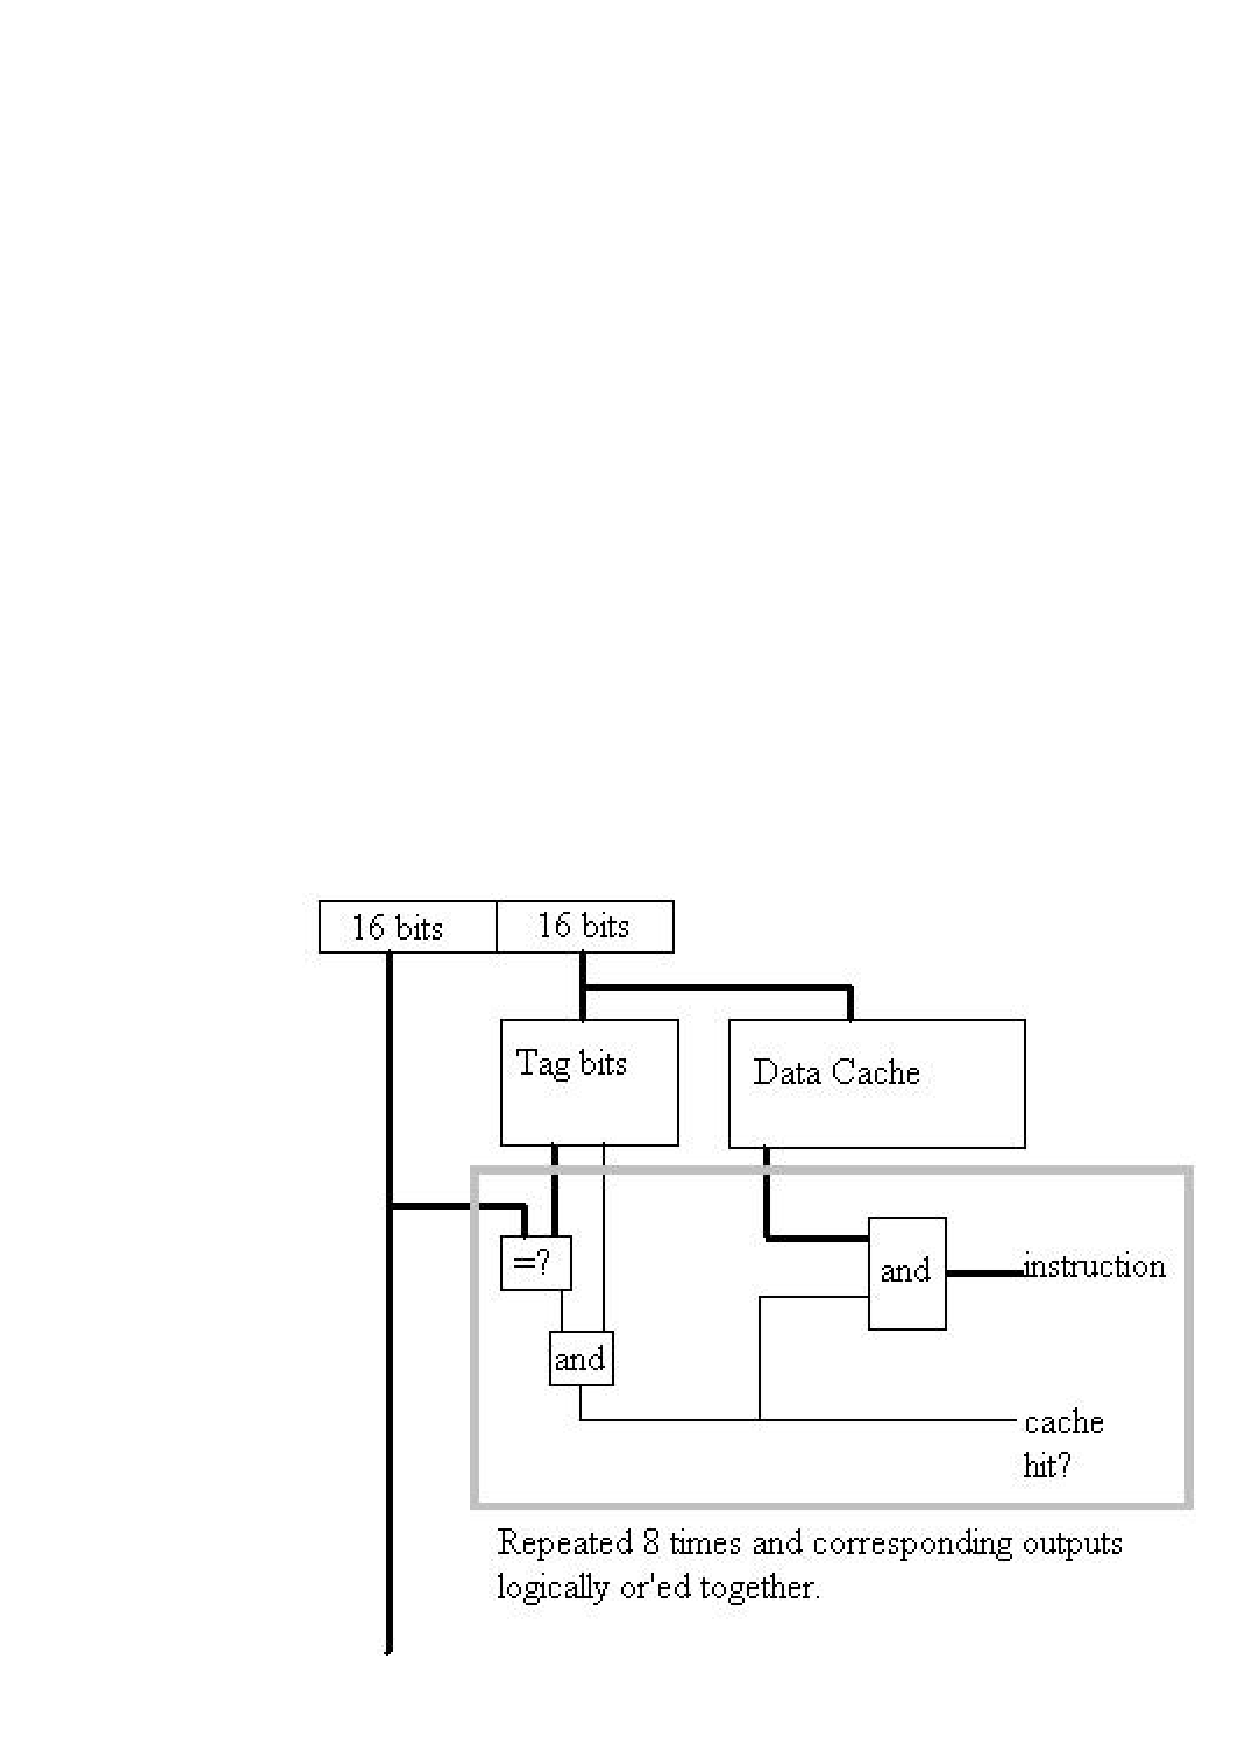
\includegraphics[width=4in]{cache.png}\\
  \caption{8-Way Set Associative Cache}\label{f-8wsac}
\end{figure}

Replacement policies
\begin{description}
    \item[LRU] Least Recently Used
    \item[FIFO] First-in First-out
    \item[LFU] Least Frequently Used
    \item[Random] Random
\end{description}

\subsection{Neat Little LRU Algorithm}

Let the number of cache slots (locations) be $2^k$, then we create a matrix of bits that is $2^k\times 2^k$ (so we can associate the cache address with both a row and column).  Initially they are all cleared.  When a cache slot, say address $p$, is accessed:
\begin{enumerate}
    \item $1$'s are placed in every bit of the matrix row $p$,
    \item $0$'s are placed in every bit of the matrix column $p$.
\end{enumerate}
Note that the second step will delete one of the $1$'s you placed in the first step.

The the address that was least recently used corresponds to the number of the row that has a sum of zero.  Equivalently, the address that was least recently used corresponds to the number of the column with the largest sum.

\Example{Fully Associative Cache With 4 Slots}

For simplicity we will assume main memory has 256 ($2^8$) bytes, and the data length is 1 byte.  The cache starts empty.

\vspace{6pt}\noindent
\begin{tabular}{|c|c|c|c|c|c|c|c|}
  \hline
  \multicolumn{4}{|c|}{NLLRU} & \multicolumn{3}{|c|}{Tag Bits} & Data \\
  0 & 1 & 2 & 3 & V & D & Address & \\ \hline
  0 & 0 & 0 & 0 & 0 & 0 & 0x00 & 0x00 \\
  0 & 0 & 0 & 0 & 0 & 0 & 0x00 & 0x00 \\
  0 & 0 & 0 & 0 & 0 & 0 & 0x00 & 0x00 \\
  0 & 0 & 0 & 0 & 0 & 0 & 0x00 & 0x00 \\
  \hline
\end{tabular}
\vspace{6pt}

Address 0x1A, which contains 0x49, is accessed.

\vspace{6pt}\noindent
\begin{tabular}{|c|c|c|c|c|c|c|c|}
  \hline
  \multicolumn{4}{|c|}{NLLRU} & \multicolumn{3}{|c|}{Tag Bits} & Data \\
  0 & 1 & 2 & 3 & V & D & Address & \\ \hline
  0 & 1 & 1 & 1 & 1 & 0 & 0x1A & 0x49 \\
  0 & 0 & 0 & 0 & 0 & 0 & 0x00 & 0x00 \\
  0 & 0 & 0 & 0 & 0 & 0 & 0x00 & 0x00 \\
  0 & 0 & 0 & 0 & 0 & 0 & 0x00 & 0x00 \\
  \hline
\end{tabular}
\vspace{6pt}

Address 0x05, which contains 0x11, is accessed.

\vspace{6pt}\noindent
\begin{tabular}{|c|c|c|c|c|c|c|c|}
  \hline
  \multicolumn{4}{|c|}{NLLRU} & \multicolumn{3}{|c|}{Tag Bits} & Data \\
  0 & 1 & 2 & 3 & V & D & Address & \\ \hline
  0 & 0 & 1 & 1 & 1 & 0 & 0x1A & 0x49 \\
  1 & 0 & 1 & 1 & 1 & 0 & 0x05 & 0x11 \\
  0 & 0 & 0 & 0 & 0 & 0 & 0x00 & 0x00 \\
  0 & 0 & 0 & 0 & 0 & 0 & 0x00 & 0x00 \\
  \hline
\end{tabular}
\vspace{6pt}

Address 0x25, which contains 0xFF, is accessed.

\vspace{6pt}\noindent
\begin{tabular}{|c|c|c|c|c|c|c|c|}
  \hline
  \multicolumn{4}{|c|}{NLLRU} & \multicolumn{3}{|c|}{Tag Bits} & Data \\
  0 & 1 & 2 & 3 & V & D & Address & \\ \hline
  0 & 0 & 0 & 1 & 1 & 0 & 0x1A & 0x49 \\
  1 & 0 & 0 & 1 & 1 & 0 & 0x05 & 0x11 \\
  1 & 1 & 0 & 1 & 0 & 0 & 0x25 & 0xFF \\
  0 & 0 & 0 & 0 & 0 & 0 & 0x00 & 0x00 \\
  \hline
\end{tabular}
\vspace{6pt}

The value 0x33 is stored to address 0x05.

\vspace{6pt}\noindent
\begin{tabular}{|c|c|c|c|c|c|c|c|}
  \hline
  \multicolumn{4}{|c|}{NLLRU} & \multicolumn{3}{|c|}{Tag Bits} & Data \\
  0 & 1 & 2 & 3 & V & D & Address & \\ \hline
  0 & 0 & 0 & 1 & 1 & 0 & 0x1A & 0x49 \\
  1 & 0 & 1 & 1 & 1 & 1 & 0x05 & 0x33 \\
  1 & 0 & 0 & 1 & 0 & 0 & 0x25 & 0xFF \\
  0 & 0 & 0 & 0 & 0 & 0 & 0x00 & 0x00 \\
  \hline
\end{tabular}
\vspace{6pt}

The value 0xF5 is stored to address 0x06.

\vspace{6pt}\noindent
\begin{tabular}{|c|c|c|c|c|c|c|c|}
  \hline
  \multicolumn{4}{|c|}{NLLRU} & \multicolumn{3}{|c|}{Tag Bits} & Data \\
  0 & 1 & 2 & 3 & V & D & Address & \\ \hline
  0 & 0 & 0 & 0 & 1 & 0 & 0x1A & 0x49 \\
  1 & 0 & 1 & 0 & 1 & 1 & 0x05 & 0x33 \\
  1 & 0 & 0 & 0 & 0 & 0 & 0x25 & 0xFF \\
  1 & 1 & 1 & 0 & 1 & 1 & 0x06 & 0xF5 \\
  \hline
\end{tabular}
\vspace{6pt}

The value 0x07 is stored to address 0x07.

\vspace{6pt}\noindent
\begin{tabular}{|c|c|c|c|c|c|c|c|}
  \hline
  \multicolumn{4}{|c|}{NLLRU} & \multicolumn{3}{|c|}{Tag Bits} & Data \\
  0 & 1 & 2 & 3 & V & D & Address & \\ \hline
  0 & 1 & 1 & 1 & 1 & 1 & 0x07 & 0x07 \\
  0 & 0 & 1 & 0 & 1 & 1 & 0x05 & 0x33 \\
  0 & 0 & 0 & 0 & 0 & 0 & 0x25 & 0xFF \\
  0 & 1 & 1 & 0 & 1 & 1 & 0x06 & 0xF5 \\
  \hline
\end{tabular}
\vspace{6pt}

\subsection{Implementing LRU Algorithm}

NLLRU is a nice algorithm to learn off, but it is not a good one to build.  First off it requires over twice as many bits as is needed.  Second, it can become inconsistent if a bit flip occurs.  To understand these problems notice the LRU square is skew symmetric:
\begin{enumerate}
\item The main diagonal is always zero.
\item The lower triangular elements (lower left triangle of the LRU square) are the negated transpose (each bit is the logical not of the bit on the opposite side of the main diagonal) of the upper triangular elements (upper right triangle of the LRU square.
\end{enumerate}


\section{Memory Performance}
\subsection{Cacheless Performance}

Every memory access must go to RAM and pay the access time for RAM, which is typically around 50ns - 70ns.  Burst transfers would be hard to use, except say for a queue system on instruction loads.

\begin{example}
Consider a system, which has no cache or instruction queue, and has RAM with 50ns access time, thus,
\begin{eqnarray}
T_{data} &=& 50ns
T_{inst} &=& 50ns
\end{eqnarray}
What is the effect on the CPI of the system assuming everything else is ideal and load/stores are a quarter of all operations?


\end{example}

\subsection{Cache Performance}

We will be concerned with some basic numbers
\begin{description}
    \item[Hit Ratio (HR)] The number of cache hits over the number of lookups.
    \item[Miss Ratio (MR)] The number of cache misses over the number of lookups.
    \item[Effective Access Time (EAT or $T_{eff}$)] The average time spent in a memory access.
\end{description}

First let us consider the hit and miss ratios.  For a series of lookups, the number of hits was ``$Hit$" and the number of misses was ``$Miss$", thus $Hit+Miss=lookups$.  Given this,
\begin{eqnarray*}
  HR &=& \frac{Hit}{Hit+Miss} \\
  MR &=& \frac{Miss}{Hit+Miss} \\
  1 &=& HR+MR
\end{eqnarray*}

thus,

\begin{eqnarray*}
  T_{eff} &=& \frac{Hit\times T_{Hit}+Miss\times T_{Miss}}{Hit+Miss} \\
          &=& HR\times T_{Hit}+MR\times T_{Miss}.
\end{eqnarray*}

Usually, the miss time is the access time ($T_{Hit}$), plus a miss penalty (say $T_{Penalty}$).

\begin{eqnarray*}
  T_{Miss}&=& T_{Hit}+T_{Penalty} \\
  T_{eff} &=& HR\times T_{Hit}+MR\times T_{Miss} \\
          &=& HR\times T_{Hit}+MR\times (T_{Hit}+T_{Penalty}) \\
          &=& (HR+MR)\times T_{Hit}+MR\times T_{Penalty} \\
          &=& T_{Hit}+MR\times T_{Penalty}
\end{eqnarray*}





\vspace{.1in}\noindent
\textbf{Example}


Use the following chart to show the state of a 4 location, 2-Way associative cache, that uses LRU.  If a location has a number printed in it, the address is valid, if no number appears the contents are invalid.  For simplicity the computer only has 16 locations in memory.  If the cache takes 5ns to access and RAM takes 60ns, what is the effective access time given the sequence?

\begin{tabular}{|l|c|c|c|c|c|c|c|c|c|c|c|} \hline
Time              & 0 & 1 & 2 & 3 & 4 & 5 & 6 & 7 & 8 & 9 & 10 \\ \hline
Lookup Address    & - & 2 & 5 & 6 & B & 5 & 2 & 2 & B & C & 5  \\ \hline
Cache location 00 & A &   &   &   &   &   &   &   &   &   &    \\ \hline
Cache location 01 & B &   &   &   &   &   &   &   &   &   &    \\ \hline
Cache location 10 &   &   &   &   &   &   &   &   &   &   &    \\ \hline
Cache location 11 &   &   &   &   &   &   &   &   &   &   &    \\ \hline
\end{tabular}

{\color{ans}
\begin{tabular}{|l|c|c|c|c|c|c|c|c|c|c|c|} \hline
Time              & 0 & 1 & 2 & 3 & 4 & 5 & 6 & 7 & 8 & 9 & 10 \\ \hline
Lookup Address    & - & 2 & 5 & 6 & B & 5 & 2 & 2 & B & C & 5  \\ \hline
Cache location 00 & A & A & A & 6 & 6 & 6 & 6 & 6 & 6 & C & C  \\ \hline
Cache location 01 & B & B & B & B & B & B & B & B & B & B & B  \\ \hline
Cache location 10 &   & 2 & 2 & 2 & 2 & 2 & 2 & 2 & 2 & 2 & 2  \\ \hline
Cache location 11 &   &   & 5 & 5 & 5 & 5 & 5 & 5 & 5 & 5 & 5  \\ \hline
\end{tabular}

MR=.4

\beqn
T_{eff}
 &=& T_{cache}+MR(T_{RAM}) \\
 &=& 5 ns+.4(60 ns) \\
 &=& 29 ns
\eeqn
}



\section{Virtual Memory}

A 32-bit virtual memory system has a 64KB page size, and 1 GB of RAM.  How large is the physical page number in bits? Assuming that the each entry in the table is word aligned, how large is the lookup table in bytes?

{\color{ans}
64KB = $2^{16}$

1GB = $2^{30}$

So the physical page number takes 30-16=14 bits or almost 2B to store in the table.  We also need to add memory protection, ownership, validity, location, etc.  I will assume that I can fit all this in 4B.

The table size is $2^{(32-16)}\times 4 B = 2^{18} B = 256 KB$
} 
\input{Kohw_control}
\part{Performance}
\input{Kohw_perf}
\input{Kohw_ilp}
\input{Kohw_pipeline}
\chapter{Tomasulo}\label{c-tomasulo}


\section{Multiple Issue Tomasulo}

To illustrate the method we will consider a simple piece of code.
\begin{verbatim}
  loop:
    mul  $t4,$t2
    mflo $t4
    subi $t3,$t3,1
    bgtz $t3,loop
\end{verbatim}
This code will calculate $ \$t4 = \$t2^{\$t3}$, assuming $\$t4=1$ initially and $\$t2>0$ and $\$t3>1$.

Further lets assume add/sub/move takes 1 cycle of execution, multiply takes 2 cycles, and branches take 2 cycle.  The branch predictor will always predict branch taken in this example.  Let's schedule this for our machine.


\noindent
\begin{tabular}{p{4in}p{2in}}
Cycle 1 & \\ \hline \hline

\noindent
\begin{tabular}{rlp{1in}lll}
\multicolumn{6}{c}{Reorder Buffer} \\
Entry & Busy & Instruction       & State & Destination & Value \\ \hline
 1    & yes  & mul  \$t4,\$t2    & Issue & \$Hi, \$Lo  &       \\
 2    & yes  & mflo \$t4         & Issue & \$t4        &       \\
 3    &      &                   &       &             &       \\
 4    &      &                   &       &             &       \\
 5    &      &                   &       &             &       \\
 6    &      &                   &       &             &       \\
 7    &      &                   &       &             &       \\
 8    &      &                   &       &             &       \\
 9    &      &                   &       &             &       \\
10    &      &                   &       &             &       \\
\end{tabular} &

\begin{tabular}{llll}
\multicolumn{4}{c}{Registers} \\
Field & Data & Reorder & Busy \\ \hline
\$t0  &      &         &      \\
\$t1  &      &         &      \\
\$t2  & 5    &         &      \\
\$t3  & 2    &         &      \\
\$t4  & 1    & \#2     & yes  \\
\$t5  &      &         &      \\
\$t6  &      &         &      \\
\$t7  &      &         &      \\
\$t8  &      &         &      \\
\$t9  &      &         &      \\
\end{tabular} \\

\noindent
\begin{tabular}{lllllllll}
\multicolumn{9}{c}{Reservation Station} \\
Name & Busy & Op   & $V_1$ & $V_2$ & $S_1$ & $S_2$ & Dest & A \\ \hline
Add1 &      & mflo &       &       & \#1   &       & \#2  &   \\
Add2 &      &      &       &       &       &       &      &   \\
Add3 &      &      &       &       &       &       &      &   \\
Add4 &      &      &       &       &       &       &      &   \\ \hline
Mul1 &      & mul  & 1     & 5     &       &       & \#1  &   \\
Mul2 &      &      &       &       &       &       &      &   \\ \hline
Br1  &      &      &       &       &       &       &      &   \\
Br2  &      &      &       &       &       &       &      &   \\
\end{tabular} & \\
\end{tabular}






\noindent
\begin{tabular}{p{4in}p{2in}}
Cycle 2 & \\ \hline \hline

\begin{tabular}{rlp{1in}lll}
\multicolumn{6}{c}{Reorder Buffer} \\
Entry & Busy & Instruction        & State & Destination & Value \\ \hline
 1    & yes  & mul  \$t4,\$t2     & Exec  & \$Hi, \$Lo  &       \\
 2    & yes  & mflo \$t4          & Issue & \$t4        &       \\
 3    & yes  & subi \$t3,\$t3,1   & Issue & \$t3        &       \\
 4    & yes  & bgtz \$t3,loop     & Issue &             &       \\
 5    &      &                    &       &             &       \\
 6    &      &                    &       &             &       \\
 7    &      &                    &       &             &       \\
 8    &      &                    &       &             &       \\
 9    &      &                    &       &             &       \\
10    &      &                    &       &             &       \\
\end{tabular} &

\begin{tabular}{llll}
\multicolumn{4}{c}{Registers} \\
Field & Data & Reorder & Busy \\ \hline
\$t0  &      &         &      \\
\$t1  &      &         &      \\
\$t2  & 5    &         &      \\
\$t3  & 2    & \#3     & yes  \\
\$t4  & 1    & \#2     & yes  \\
\$t5  &      &         &      \\
\$t6  &      &         &      \\
\$t7  &      &         &      \\
\$t8  &      &         &      \\
\$t9  &      &         &      \\
\end{tabular} \\

\noindent
\begin{tabular}{lllllllll}
\multicolumn{9}{c}{Reservation Station} \\
Name & Busy & Op   & $V_1$ & $V_2$ & $S_1$ & $S_2$ & Dest & A \\ \hline
Add1 &      & mflo &       &       & \#1   &       & \#2  &   \\
Add2 &      & subi & 2     & 1     &       &       & \#3  &   \\
Add3 &      &      &       &       &       &       &      &   \\
Add4 &      &      &       &       &       &       &      &   \\ \hline
Mul1 & yes  & mul  & 1     & 5     &       &       & \#1  &   \\
Mul2 &      &      &       &       &       &       &      &   \\ \hline
Br1  &      & bgtz &       &       & \#3   &       & \#4  &   \\
Br2  &      &      &       &       &       &       &      &   \\
\end{tabular} &  \\
\end{tabular}






\noindent
\begin{tabular}{p{4in}p{2in}}
Cycle 3 & \\ \hline \hline

\begin{tabular}{rlp{1in}lll}
\multicolumn{6}{c}{Reorder Buffer} \\
Entry & Busy & Instruction        & State & Destination & Value \\ \hline
 1    & yes  & mul  \$t4,\$t2     & Exec  & \$Hi, \$Lo  &       \\
 2    & yes  & mflo \$t4          & Issue & \$t4        &       \\
 3    & yes  & subi \$t3,\$t3,1   & Exec  & \$t3        &       \\
 4    & yes  & bgtz \$t3,loop     & Issue &             &       \\
 5    & yes  & mul  \$t4,\$t2     & Issue & \$Hi, \$Lo  &       \\
 6    & yes  & mflo \$t4          & Issue & \$t4        &       \\
 7    &      &                    &       &             &       \\
 8    &      &                    &       &             &       \\
 9    &      &                    &       &             &       \\
10    &      &                    &       &             &       \\
\end{tabular} &

\begin{tabular}{llll}
\multicolumn{4}{c}{Registers} \\
Field & Data & Reorder & Busy \\ \hline
\$t0  &      &         &      \\
\$t1  &      &         &      \\
\$t2  & 5    &         &      \\
\$t3  & 2    & \#3     & yes  \\
\$t4  & 1    & \#6     & yes  \\
\$t5  &      &         &      \\
\$t6  &      &         &      \\
\$t7  &      &         &      \\
\$t8  &      &         &      \\
\$t9  &      &         &      \\
\end{tabular} \\

\noindent
\begin{tabular}{lllllllll}
\multicolumn{9}{c}{Reservation Station} \\
Name & Busy & Op   & $V_1$ & $V_2$ & $S_1$ & $S_2$ & Dest & A \\ \hline
Add1 &      & mflo &       &       & \#1   &       & \#2  &   \\
Add2 & yes  & subi & 2     & 1     &       &       & \#3  &   \\
Add3 &      & mflo &       &       & \#5   &       & \#6  &   \\
Add4 &      &      &       &       &       &       &      &   \\ \hline
Mul1 & yes  & mul  & 1     & 5     &       &       & \#1  &   \\
Mul2 &      & mul  &       & 5     & \#2   &       & \#5  &   \\ \hline
Br1  &      & bgtz &       &       & \#3   &       & \#4  &   \\
Br2  &      &      &       &       &       &       &      &   \\
\end{tabular} &  \\
\end{tabular}






\noindent
\begin{tabular}{p{4in}p{2in}}
Cycle 4 & \\ \hline \hline

\begin{tabular}{rlp{.9in}lll}
\multicolumn{6}{c}{Reorder Buffer} \\
Entry & Busy & Instruction        & State & Destination & Value \\ \hline
 1    & no   & mul  \$t4,\$t2     & Commit& \$Hi, \$Lo  & 5     \\
 2    & yes  & mflo \$t4          & Exec  & \$t4        &       \\
 3    & no   & subi \$t3,\$t3,1   & done  & \$t3        & 1     \\
 4    & yes  & bgtz \$t3,loop     & Exec  &             &       \\
 5    & yes  & mul  \$t4,\$t2     & Issue & \$Hi, \$Lo  &       \\
 6    & yes  & mflo \$t4          & Issue & \$t4        &       \\
 7    & yes  & subi \$t3,\$t3,1   & Issue & \$t3        &       \\
 8    & yes  & bgtz \$t3,loop     & Issue &             &       \\
 9    &      &                    &       &             &       \\
10    &      &                    &       &             &       \\
\end{tabular} &

\begin{tabular}{llll}
\multicolumn{4}{c}{Registers} \\
Field & Data & Reorder & Busy \\ \hline
\$t0  &      &         &      \\
\$t1  &      &         &      \\
\$t2  & 5    &         &      \\
\$t3  & 1    & \#7     & yes  \\
\$t4  & 1    & \#6     & yes  \\
\$t5  &      &         &      \\
\$t6  &      &         &      \\
\$t7  &      &         &      \\
\$t8  &      &         &      \\
\$t9  &      &         &      \\
\end{tabular} \\

\noindent
\begin{tabular}{lllllllll}
\multicolumn{9}{c}{Reservation Station} \\
Name & Busy & Op   & $V_1$ & $V_2$ & $S_1$ & $S_2$ & Dest & A \\ \hline
Add1 & yes  & mflo & 5     &       &       &       & \#2  &   \\
Add2 &      & subi & 1     & 1     &       &       & \#7     &   \\
Add3 &      & mflo &       &       & \#5   &       & \#6  &   \\
Add4 &      &      &       &       &       &       &      &   \\ \hline
Mul1 &      &      &       &       &       &       &      &   \\
Mul2 &      & mul  &       & 5     & \#2   &       & \#5  &   \\ \hline
Br1  & yes  & bgtz & 1     &       &       &       & \#4  &   \\
Br2  &      & bgtz &       & \#7   &       &       & \#8  &   \\
\end{tabular} &  \\
\end{tabular}






\noindent
\begin{tabular}{p{4in}p{2in}}
Cycle 5 & \\ \hline \hline

\begin{tabular}{rlp{.9in}lll}
\multicolumn{6}{c}{Reorder Buffer} \\
Entry & Busy & Instruction        & State & Destination & Value \\ \hline
 1    &      &                    &       &             &       \\
 2    & no   & mflo \$t4          & Commit& \$t4        & 5     \\
 3    & no   & subi \$t3,\$t3,1   & Commit& \$t3        & 1     \\
 4    & yes  & bgtz \$t3,loop     & Exec  &             &       \\
 5    & yes  & mul  \$t4,\$t2     & Exec  & \$Hi, \$Lo  &       \\
 6    & yes  & mflo \$t4          & Issue & \$t4        &       \\
 7    & yes  & subi \$t3,\$t3,1   & Exec  & \$t3        &       \\
 8    & yes  & bgtz \$t3,loop     & Issue &             &       \\
 9    & yes  & mul  \$t4,\$t2     & Issue & \$Hi, \$Lo  &       \\
10    & yes  & mflo \$t4          & Issue & \$t4        &       \\
\end{tabular} &

\begin{tabular}{llll}
\multicolumn{4}{c}{Registers} \\
Field & Data & Reorder & Busy \\ \hline
\$t0  &      &         &      \\
\$t1  &      &         &      \\
\$t2  & 5    &         &      \\
\$t3  & 1    & \#7     & yes  \\
\$t4  & 5    & \#10     & yes  \\
\$t5  &      &         &      \\
\$t6  &      &         &      \\
\$t7  &      &         &      \\
\$t8  &      &         &      \\
\$t9  &      &         &      \\
\end{tabular} \\

\noindent
\begin{tabular}{lllllllll}
\multicolumn{9}{c}{Reservation Station} \\
Name & Busy & Op   & $V_1$ & $V_2$ & $S_1$ & $S_2$ & Dest & A \\ \hline
Add1 &      & mflo &       &       & \#9   &       & \#10 &   \\
Add2 & yes  & subi & 1     & 1     &       &       & \#7  &   \\
Add3 &      & mflo &       &       & \#5   &       & \#6  &   \\
Add4 &      &      &       &       &       &       &      &   \\ \hline
Mul1 &      & mul  &       & 5     & \#6   &       & \#9  &   \\
Mul2 & yes  & mul  & 5     & 5     &       &       & \#5  &   \\ \hline
Br1  & yes  & bgtz & 1     &       &       &       & \#4  &   \\
Br2  &      & bgtz &       & \#7   &       &       & \#8  &   \\
\end{tabular} &  \\
\end{tabular}






\noindent
\begin{tabular}{p{4in}p{2in}}
Cycle 6 & \\ \hline \hline

\begin{tabular}{rlp{.9in}lll}
\multicolumn{6}{c}{Reorder Buffer} \\
Entry & Busy & Instruction        & State & Destination & Value \\ \hline
 1    & yes  & subi \$t3,\$t3,1   & Issue & \$t3        &       \\
 2    & yes  & bgtz \$t3,loop     & Issue &             &       \\
 3    &      &                    &       &             &       \\
 4    & no   & bgtz \$t3,loop     & Commit&             &       \\
 5    & yes  & mul  \$t4,\$t2     & Exec  & \$Hi, \$Lo  &       \\
 6    & yes  & mflo \$t4          & Issue & \$t4        &       \\
 7    & no   & subi \$t3,\$t3,1   & Done  & \$t3        & 0     \\
 8    & yes  & bgtz \$t3,loop     & Issue &             &       \\
 9    & yes  & mul  \$t4,\$t2     & Issue & \$Hi, \$Lo  &       \\
10    & yes  & mflo \$t4          & Issue & \$t4        &       \\
\end{tabular} &

\begin{tabular}{llll}
\multicolumn{4}{c}{Registers} \\
Field & Data & Reorder & Busy \\ \hline
\$t0  &      &         &      \\
\$t1  &      &         &      \\
\$t2  & 5    &         &      \\
\$t3  & 1    & \#1     & yes  \\
\$t4  & 5    & \#10    & yes  \\
\$t5  &      &         &      \\
\$t6  &      &         &      \\
\$t7  &      &         &      \\
\$t8  &      &         &      \\
\$t9  &      &         &      \\
\end{tabular} \\

\noindent
\begin{tabular}{lllllllll}
\multicolumn{9}{c}{Reservation Station} \\
Name & Busy & Op   & $V_1$ & $V_2$ & $S_1$ & $S_2$ & Dest & A \\ \hline
Add1 &      & mflo &       &       & \#9   &       & \#10 &   \\
Add2 &      & subi & 0     & 1     &       &       & \#1  &   \\
Add3 &      & mflo &       &       & \#5   &       & \#6  &   \\
Add4 &      &      &       &       &       &       &      &   \\ \hline
Mul1 &      & mul  &       & 5     & \#6   &       & \#9  &   \\
Mul2 & yes  & mul  & 5     & 5     &       &       & \#5  &   \\ \hline
Br1  &      & bgtz &       &       & \#2   &       & \#2  &   \\
Br2  & yes  & bgtz & 0     &       &       &       & \#8  &   \\
\end{tabular} &  \\
\end{tabular}






\noindent
\begin{tabular}{p{4in}p{2in}}
Cycle 7 & \\ \hline \hline

\begin{tabular}{rlp{.9in}lll}
\multicolumn{6}{c}{Reorder Buffer} \\
Entry & Busy & Instruction        & State & Destination & Value \\ \hline
 1    & yes  & subi \$t3,\$t3,1   & Issue & \$t3        &       \\
 2    & yes  & bgtz \$t3,loop     & Issue &             &       \\
 3    &      &                    &       &             &       \\
 4    &      &                    &       &             &       \\
 5    & no   & mul  \$t4,\$t2     & Commit& \$Hi, \$Lo  & 25    \\
 6    & yes  & mflo \$t4          & Exec  & \$t4        &       \\
 7    & no   & subi \$t3,\$t3,1   & Done  & \$t3        & 0     \\
 8    & yes  & bgtz \$t3,loop     & Exec  &             &       \\
 9    & yes  & mul  \$t4,\$t2     & Issue & \$Hi, \$Lo  &       \\
10    & yes  & mflo \$t4          & Issue & \$t4        &       \\
\end{tabular} &

\begin{tabular}{llll}
\multicolumn{4}{c}{Registers} \\
Field & Data & Reorder & Busy \\ \hline
\$t0  &      &         &      \\
\$t1  &      &         &      \\
\$t2  & 5    &         &      \\
\$t3  & 1    & \#1     & yes  \\
\$t4  & 5    & \#10    & yes  \\
\$t5  &      &         &      \\
\$t6  &      &         &      \\
\$t7  &      &         &      \\
\$t8  &      &         &      \\
\$t9  &      &         &      \\
\end{tabular} \\

\noindent
\begin{tabular}{lllllllll}
\multicolumn{9}{c}{Reservation Station} \\
Name & Busy & Op   & $V_1$ & $V_2$ & $S_1$ & $S_2$ & Dest & A \\ \hline
Add1 &      & mflo &       &       & \#9   &       & \#10 &   \\
Add2 &      & subi & 0     & 1     &       &       & \#1  &   \\
Add3 & yes  & mflo & 25    &       &       &       & \#6  &   \\
Add4 &      &      &       &       &       &       &      &   \\ \hline
Mul1 &      & mul  &       & 5     & \#6   &       & \#9  &   \\
Mul2 &      &      &       &       &       &       &      &   \\ \hline
Br1  &      & bgtz &       &       & \#2   &       & \#2  &   \\
Br2  & yes  & bgtz & 0     &       &       &       & \#8  &   \\
\end{tabular} &  \\
\end{tabular}






\noindent
\begin{tabular}{p{4in}p{2in}}
Cycle 8 & \\ \hline \hline

\begin{tabular}{rlp{.9in}lll}
\multicolumn{6}{c}{Reorder Buffer} \\
Entry & Busy & Instruction        & State & Destination & Value \\ \hline
 1    & yes  & subi \$t3,\$t3,1   & Exec  & \$t3        &       \\
 2    & yes  & bgtz \$t3,loop     & Issue &             &       \\
 3    & yes  & mul  \$t4,\$t2     & Issue &             &       \\
 4    & yes  & mflo \$t4          & Issue &             &       \\
 5    &      &                    &       &             &       \\
 6    &      &                    &       &             &       \\
 7    &      &                    &       &             &       \\
 8    & no   & bgtz \$t3,loop     & Flush &             &       \\
 9    & yes  & mul  \$t4,\$t2     & Exec  & \$Hi, \$Lo  &       \\
10    & yes  & mflo \$t4          & Issue & \$t4        &       \\
\end{tabular} &

\begin{tabular}{llll}
\multicolumn{4}{c}{Registers} \\
Field & Data & Reorder & Busy \\ \hline
\$t0  &      &         &      \\
\$t1  &      &         &      \\
\$t2  & 5    &         &      \\
\$t3  & 0    & \#1     & yes  \\
\$t4  & 25   & \#4     & yes  \\
\$t5  &      &         &      \\
\$t6  &      &         &      \\
\$t7  &      &         &      \\
\$t8  &      &         &      \\
\$t9  &      &         &      \\
\end{tabular} \\

\noindent
\begin{tabular}{lllllllll}
\multicolumn{9}{c}{Reservation Station} \\
Name & Busy & Op   & $V_1$ & $V_2$ & $S_1$ & $S_2$ & Dest & A \\ \hline
Add1 &      & mflo &       &       & \#9   &       & \#10 &   \\
Add2 & yes  & subi & 0     & 1     &       &       & \#1  &   \\
Add3 &      & mflo &       &       & \#3   &       & \#4  &   \\
Add4 &      &      &       &       &       &       &      &   \\ \hline
Mul1 & yes  & mul  & 25    & 5     &       &       & \#9  &   \\
Mul2 &      & mul  &       & 5     & \#10  &       & \#3  &   \\ \hline
Br1  &      & bgtz &       &       & \#2   &       & \#2  &   \\
Br2  &      &      &       &       &       &       &      &   \\
\end{tabular} &  \\
\end{tabular}

At this point the buffers and stations will be flushed, the executions cancelled, and the registers not updated (they are at the right point).  New commands will be loaded from after the branch, and execution proceeds normally. 
\input{Kohw_tlp}

\part{Appendices}
\appendix
\input{Kohw_machine_examples}
\chapter{Encryption}
\label{c-encryption}

\section{Modular Arithmetic}

\subsection{Congruence}

We say $a$ is congruent to $b$ modulus $n$ when $a-b$ is divisible by $n$.  In mathematical notation, we write $a \equiv b \qquad(\mod n)\quad\Leftrightarrow\quad a-b= kn$ for some integer $k$.  Several important properties of congruence are
\begin{enumerate}
\item $a \equiv a \qquad(\mod n)$
\item $a \equiv b \qquad(\mod n)\qquad\Rightarrow\qquad b \equiv a \qquad(\mod n)$
\item $\{\{a \equiv b \qquad(\mod n)\}\,\cdot\,\{b \equiv c \qquad(\mod n)\}\}
       \qquad\Rightarrow\qquad a \equiv c \qquad(\mod n)$
\end{enumerate}

\begin{example}
\beqn
8&\equiv&29\qquad(\mod 7) \\
8-29 &=& -21 \\
&=& (-3)7
\eeqn


\beqn
9&\equiv&-15\qquad(\mod 6) \\
9-(-15) &=& 24 \\
&=& (4)6
\eeqn
\end{example}

\subsection{Modulus}

Invariably confusion happens with integer division, modulus, and remainder involving negative numbers.  The problem arises in the basic definition.  For a dividend, $a\in\mathbb{Z}$ and a divisor, $b\in\mathbb{Z}$, the quotient, $q$ and remainder $r$ must satisfy
\begin{enumerate}
\item $\{r,q\}\in\mathbb{Z}$,
\item $a=b*q+r$,
\item $|r|<|d|$.
\end{enumerate}
The problem comes with the last requirement, because many choices can be made.  The three most justifiable definitions are below\footnote{other definitions exist such as ceiling division and rounding division, but they do not correspond to the what most people think of division for positive numbers.  Note, from the requirements nothing says $5/2=3r-1$ but this is hardly what most people would think of, and thus would probably not be programmed very well.}
\begin{enumerate}
\item Truncate division preserves the magnitudes of the quotient and remainder, independent of the signs of the dividend and divisor.  This forces the remainder to have the same sign as the dividend.
\item Floor division forces the remainder to have the same sign as the divisor.
\item Euclidean division defines $r\geq 0$ and thus ensures $b\times q\leq a$.
\end{enumerate}
Each is defensible.


\subsubsection{Truncate}
Remainder's definition is based off the definition of integer division.  Integer division, $a/b$, is defined for positive $a$ and $b$ to be the number $q$ such that
\begin{enumerate}
\item $b\times q\leq a$,
\item $b\times (q+1)\geq a$.
\end{enumerate}
When negative numbers are allowed the following requirement is added
\begin{enumerate}
\item[3] $(-a)/b = a/(-b) = -(a/b)$,
\end{enumerate}
still for $a$ and $b$ positive.  One could summarize this as:
\beqn
c/d &=& \sign(c)\sign(d)(|c|/|d|)
\eeqn
Given we now have quotient or integer division defined we can then define remainder such that
\beqn
a &=& a/b + a rem b \\
a rem b &=& a-a/b.
\eeqn
Note that the sign of the remainder is the same as the 

\begin{example}
Consider the following:

\begin{tabular}{cc}
\begin{minipage}{2in}
\beqn
5/2 &=& 2 \\
(-5)/2 &=& -2 \\
5/(-2) &=& -2 \\
(-5)/(-2) &=& 2
\eeqn
\end{minipage}
&
\begin{minipage}{2in}
\beqn
5 rem 2 &=& 1 \\
(-5) rem 2 &=& -1 \\
5 rem (-2) &=& 1 \\
(-5) rem (-2) &=& -1
\eeqn
\end{minipage} \\
\end{tabular}
\end{example}



\subsection{Addition}

$\{\{a \equiv b \qquad(\mod n)\}\,\cdot\,\{c \equiv d \qquad(\mod n)\}\} \qquad\Rightarrow\qquad a+c \equiv b+d \qquad(\mod n)$

\subsection{Additive Inverse}

\beqn
a + \bar a &\equiv& 0 \quad(\mod n) \\
a + \bar a &=& k n, \qquad k\in\mathbb{Z} \\
\bar a &=& k n-a, \qquad k\in\mathbb{Z}
\eeqn

\begin{example}
Find the additive inverse(s) of 3 mod 7.

\beqn
\bar a &=& k n-a, \qquad k\in\mathbb{Z} \\
&=& 7k -3, \qquad k\in\mathbb{Z}
\eeqn

\begin{tabular}{lll}
k & $\bar a$ & $(3+\bar a)\mod 7$ \\ \hline
1 & 4        & $(3+4)\mod 7=0$ \\
2 & 11       & $(3+11)\mod 7=0$ \\
3 & 18       & $(3+18)\mod 7=0$ \\
4 & 25       & $(3+25)\mod 7=0$ \\
\vdots & \vdots \\
\end{tabular}
\end{example}

\subsection{Multiplication}

$\{\{a \equiv b \qquad(\mod n)\}\,\cdot\,\{c \equiv d \qquad(\mod n)\}\} \qquad\Rightarrow\qquad ac \equiv bd \qquad(\mod n)$



\subsection{Multiplicative Inverse}

\beqn
a \bar a &\equiv& 1 \quad(\mod n) \\
a \bar a &=& 1+k n, \qquad k\in\mathbb{Z} \\
\bar a &=& \frac{1+k n}{a}, \qquad k\in\mathbb{Z}
\eeqn
Let $k_1+a k_2=k$ for $k_1$ and $k_2$ positive integers.
\beqn
\bar a &=& \frac{1+k n}{a}, \qquad k\in\mathbb{Z} \\
 &=& \frac{1+k_1 n+ a k_2 n}{a}, \qquad k_1,k_2\in\mathbb{Z^+} \\
 &=& \frac{1+k_1 n}{a}+k_2 n, \qquad k_1,k_2\in\mathbb{Z^+}
\eeqn
We need $a$ to divide $1+k_1n$, which means it divides with no remainder (aka divides evenly).  Consider what would happen if $gcd(a,n)=a_1>1$, thus $a=a_1a_2$ and $n=a_1n_2$ for $a_1$, $a_2$, and $n_2$ positive integers.  If $a_1$ is a factor of $n$ then it is also a factor of $k_1n$  If $a_1$ is a factor of $k_1n$ then it cannot be a factor of $k_1n+1$ (it evenly divides $k_1n$ and $k_1n+k_1$ but nothing in between).

Now assume $gcd(a,n)=1$.  For $a$ to divide $1+k_1n$ implies $ak_3=1+k_1n$ for some positive integer $k_3$.

\begin{example}
Find the multiplicative inverse(s) of 3 mod 7.

\beqn
\bar a &=& \frac{1+k n}{a}, \qquad k\in\mathbb{Z} \\
&=& \frac{1+7k}{3}, \qquad k\in\mathbb{Z}
\eeqn

\begin{tabular}{lll}
k & $\bar a$          & $(3+\bar a)\mod 7$ \\ \hline
1 & $\frac{8}{3}$ no  &  \\
2 & $\frac{15}{3}=5$  & $(3\times 5)\mod 7=1$ \\
3 & $\frac{22}{3}$ no &  \\
4 & $\frac{29}{3}$ no &  \\
5 & $\frac{36}{3}=12$ & $(3\times 12)\mod 7=1$ \\
\vdots & \vdots \\
\end{tabular}
\end{example}

\section{Affine Encryption Program}\label{s-affine}

Affine encryption is one of the simplest methods for doing encryption.  Let $P_i$ be the $i^{th}$ character in the plain text message, and let $C_i$ be the corresponding encoded character.  Let there be $n$ possible characters to encode, then the basic idea is to pick two numbers $(a,b)$ to encode a message such that $\gcd(a,n)=1$ (so $a$ has an inverse).  No requirement on $b$ is needed if your modulus function has been encoded correctly.  The encoded character can then be found by
\begin{eqnarray*}
  a\times P_i +b &=& C_i \mod n.
\end{eqnarray*}
Note that the "$\mod n$" at the end says the equation holds in $\Zed_n$, the set of integers mod $n$ with appropriately defined arithmetic.

To decrypt the message, the equation
\begin{eqnarray*}
  \bar a\times (C_i +d) &=& P_i \mod n
\end{eqnarray*}
is used.  The term $\bar a$ is the inverse of $a$ in $\Zed_n$, which is found by solving
\begin{eqnarray*}
  a\times\bar a &=& 1 \mod n \\
   & \textbf{or} & \\
  a\times\bar a &=& m\times n+1.
\end{eqnarray*}
Note that $m$ is any whole number.  The term $d$ is the additive inverse of $b$ in $\Zed_n$, which is found by solving
\begin{eqnarray*}
  d=n-(b \mod n).
\end{eqnarray*}

We can summarize this by saying an affine cipher is an encryption technique that encodes using three integers: $a$, $b$, and $n$.  If $plain$ is the character to be encoded (with `A'=0 and `Z'=25) then $code=(a*plain+b) \mod n$.  Decoding is also done using three integers: $c$, $d$, and $n$.  If $code$ is the character to be encoded (with `A'=0 and `Z'=25) then $plain=(c*(code+d)) \mod n$.  The requirements on $(a,b,c,d,n)$ are:
\begin{itemize}
    \item $\gcd(a,n)=1$
    \item $(ac) \mod n = 1$
    \item $(b+d) \mod n = 0$
\end{itemize}
Below is C code to implement a particular case of affine cyphers.
\begin{verbatim}

char affine_encode(char plain){
    // affine codes capital letter in plain using a=5, b=12 thus this is modulo 26
    int iCode, iPlain, a=3,b=0;

    // convert char to integer and shift so A=0
    iPlain=int(plain)-65;

    // do the encoding
    iCode = (a*iPlain+b)%26;

    // return the result as a char
    return char(iCode+65);
}

char affine_decode(char code){
    // affine decodes capital letter in plain using c=21, d=8 thus this is modulo 26
    int iCode, iPlain, c=9, d=0;

    // convert char to integer and shift so A=0
    iCode=int(code)-65;

    // do the decoding
    iPlain = (c*(iCode+d))%26;

    // return the result as a char
    return char(iPlain+65);
}
\end{verbatim} 
\chapter{Projects for CSCI 313}
\label{c-proj}

\section{Data Compression/Uncompression}

Write in SPARC assembly a program that would use Huffman coding to compress an ASCII file and then uncompress the same file using Huffman coding in reverse.

The following table presents the relative frequencies of letters in the English language.

\begin{tabular}{ll|ll|ll}
  Letter & Freq.  & Letter & Freq.  & Letter  & Freq. \\ \hline
  A      & 0.0681 & K      & 0.0037 & U       & 0.0272 \\
  B      & 0.0123 & L      & 0.0355 & V       & 0.0095 \\
  C      & 0.0288 & M      & 0.0257 & W       & 0.0144 \\
  D      & 0.0406 & N      & 0.0628 & X       & 0.0025 \\
  E      & 0.1205 & O      & 0.0671 & Y       & 0.0146 \\
  F      & 0.0283 & P      & 0.0210 & Z       & 0.0004 \\
  G      & 0.0134 & Q      & 0.0009 & space   & 0.0600 \\
  H      & 0.0580 & R      & 0.0514 & .       & 0.0400 \\
  I      & 0.0577 & S      & 0.0496 & newline & 0.0090 \\
  J      & 0.0018 & T      & 0.0752 &         &  \\
\end{tabular}

You must first derive the decode tree using the above table and then create the translation table manually.  The translation table can then be used to compress and decompress ASCII files.

\section{Postfix Expression Evaluator}

The project is to write in SPARC assembly a program that would evaluate a postfix expression.  The postfix expression will contain the following arithmetic operators:
\begin{description}
    \item[+] binary addition
    \item[-] binary subtration
    \item[*] binary multiplication
    \item[/] binary division
    \item[?] unary increment
    \item[!] unary decrement
    \item[$\sim$] unary negation
\end{description}

The infix expression
\beqn
5 \, / \, 2 \, ? \, + \, 4 \, * \, 6 \, - \, 1 \, * \, 3
\eeqn
is equivalent to the postfix expression
\beqn
5 \, 2 \, ? \, / \, 4 \, 6 \, * \, + \, 1 \, 3 \, * \, -.
\eeqn

The following is the algorithm for the postfix expression evaluator.

\begin{tabbing}
          aaa \= aaa \= aaa \= aaa \= aaa \= aaa  \kill
          % \> for next tab, \\ for new line...
          procedure EVAL (E) \\
            \> /* \> Evaluate the postfix expression E.  It is assumed  \\
            \>    \> that the last character in E is a NUL.  A procedure  \\
            \>    \> NEXT-TOKEN is used to extract from E the next token.   \\
            \>    \> A token array STACK(1:n) is used as a stack.  \\
            \> */  \\
            \> \\
            \> top $\leftarrow$ 0 \\
            \> loop \\
            \>    \> x $\leftarrow$ NEXT-TOKEN(E) \\
            \>    \>   \> case \\
            \>    \>   \> :x = NUL: return \\
            \>    \>   \> :x is an operand: call PUSH(x,STACK) \\
            \>    \>   \> :else: remove the correct number of opeands \\
            \>    \>   \>   \> for operator x from STACK, perform \\
            \>    \>   \>   \> the operation and store the result,  \\
            \>    \>   \>   \> if any, onto the STACK \\
            \>    \>   \> end \\
            \> forever \\
          end EVAL
\end{tabbing}

\chapter{Mini: ALU}
\label{c-lab-alu}

\section{Half Adder}

Let's begin this section by considering a simple problem of how to design an adder for two bits.  Call the bits ``a" and ``b".  The sum will take two bits to hold, ``carry" (c) and ``sum" (s).

\vspace{.1in}
\begin{tabular}{rcrcrcrcr}
 a & &  0 & &  0 & &  1 & &  1 \\
+b & & +0 & & +1 & & +0 & & +1 \\ \cline{1-1} \cline{3-3} \cline{5-5} \cline{7-7} \cline{9-9}
cs & & 00 & & 01 & & 01 & & 10 \\
\end{tabular}

\vspace{.1in}
\noindent
We can express this as a table.

\vspace{.1in}
\begin{tabular}{c|c||c|c}
a & b & c & s \\ \hline
0 & 0 & 0 & 0 \\
0 & 1 & 0 & 1 \\
1 & 0 & 0 & 1 \\
1 & 1 & 1 & 0 \\
\end{tabular}

\vspace{.1in}
\noindent
From the table we can recognize that $c=a\cdot b$ and $s=a\oplus b$.

\begin{verbatim}
// name: half_adder
// desc: adds two single bits and outputs the the two bit answer [C,S]
// date:
// by  :
module half_adder(C,S,a,b); // you list all inputs and outputs, by convention outputs go first
  input  a, b;              // this tells the compiler which lines are inputs, outputs, and inouts
  output C, S;

  parameter delay=1;        // this creates a parameter that can be changed when it is
                            // instantiated, default value is 1

  and #delay carry(C,a,b);  // this instantiates a gate, sets its parameter to delay (time delay)
  xor #delay sum(S,a,b);    //  and passes the wires a,b as inputs to the gate and gets the
                            //  gate driven wires C or S as outputs
endmodule
\end{verbatim}

\section{Full Adders}

We really want to have a way to add three bits, the two bits of the current digit and one bit carried from the previous sum.

\begin{tabular}{r}
 $c_{prev}$ \\
 a \\
+b \\ \hline
cs \\
\end{tabular}

As before we could make a table, but it is not necessary we can just add in pairs:

\begin{tabular}{rcr}
half-adder 1 & & half-adder 2 \\
 a           & & $c_{prev}$ \\
+b           & & +$s_i$     \\ \cline{1-1} \cline{3-3}
$c_is_i$     & & $c_js$     \\
\end{tabular}

and we \textbf{or} (as in the gate) the two intermediate carries together ($c=c_i+c_j$).  Thus we can implement it as two half adders.  Create a module ``full\_adder" and instantiate two half adders per the table to generate the sum and the intermediate carries, then combine the carries with an or gate to generate the carry out.  Make sure you also include the parameter delay, or the next level up will not be able to change the levels below it.

\section{Adder-Subtractor}

In the previous section you made a module of a full adder.  In this preparation you will make a four bit adder subtractor using your full adder module.  We will add a feature called carry enable, which when set (equal 1) causes the adder-subtractor to act normally, but when unset (equal 0) stops the carry from being passed, and thus turn the adder-subtractor into an \textbf{xor} gate (from the half-adder).

\begin{enumerate}
\item Create a new module with two four bit inputs for the numbers and a four bit output for the result.  Your module should also have a carry in and a carry out line.

\begin{verbatim}
// name: four_bit_adder
// desc: four bit ripple carry adder with carry enable,
//         if C_en then [C_out,Z] = x+y+C_in
//                 else Zi = Xi xor Yi
// date:
// by  :
module four_bit_adder(Z,C_out,x,y,C_in,c_en);
  input  C_in, c_en;
  input  [3:0] x,y;
  output C_out;
  output [3:0] Z;

  parameter delay=1;        // this creates a parameter that can be changed when it is
                            // instantiated, default value is 1

endmodule
\end{verbatim}


\item Now create 7 wires to hold the intermediate carries between the full adders and the and gates that will connect them.

\item Make four instances of your full adder, being sure to pass it the delay parameter.

\item Create four \textbf{and} gates to do the carry enable logic.  Be sure to give them the parameter ``delay" so we can do timing later.  The outputs of each And gate should be connected to the carry in of one of the full adders.  One of the inputs of each and gate should be connected to C\_en.

\item Finally, connect the carry outs of the first three adders to the \textbf{and} gate of the next bit.  The first \textbf{and} gate gets C\_in.

\end{enumerate}

Test your full adder with the following module:

\begin{verbatim}
// name: test1
// desc: tests four bit ripple carry adder
// date:
// by  :
module test1();
  reg [3:0] a, b;
  reg c0, cen;
  wire [3:0] s;
  wire c4;

  // create instance of adder
  four_bit_adder #1 adder(c,c4,a,b,c0,cen);

  // set up the monitoring
  initial
  begin
    $display("A    B    C0   C4 S     Time");
    $monitor("%b   %b   %b   %b %b    %d", a,b,c0,c4,s,$time);
  end

  // run through a series of numbers
  initial
  begin
        a=4'b0000; b=4'b0000; c0=1'b0; cen=1'b1;
    #10 a=4'b0100; b=4'b0000; c0=1'b0; cen=1'b1;
    #10 a=4'b0100; b=4'b0011; c0=1'b0; cen=1'b1;
    #10 a=4'b0100; b=4'b0011; c0=1'b1; cen=1'b1;
    #10 a=4'b1100; b=4'b0011; c0=1'b1; cen=1'b1;
    #10 a=4'b1100; b=4'b0011; c0=1'b0; cen=1'b1;
    #10 a=4'b0100; b=4'b0000; c0=1'b0; cen=1'b0;
    #10 a=4'b0100; b=4'b0011; c0=1'b0; cen=1'b0;
    #10 a=4'b0100; b=4'b0011; c0=1'b1; cen=1'b0;
    #10 a=4'b1100; b=4'b0011; c0=1'b1; cen=1'b0;
    #10 a=4'b1100; b=4'b0011; c0=1'b0; cen=1'b0;
    #10 $finish;
  end

endmodule
\end{verbatim}

Once your four bit adder is working, you need to make a four bit adder subtractor from it.  See Figure 4-13 in Morris Mano, Digital Design, page 127 for a diagram of a ripple carry adder-subtractor.  For simplicity we will not calculate overflow (V).   Follow these steps:

\begin{enumerate}
\item Create a new module.

\begin{verbatim}
// name: four_bit_adder_subtractor
// desc: four bit ripple carry adder, [C_out,Z] = x+(-)y+C_in
// date:
// by  :
module four_bit_adder_subtractor(Z,C_out,x,y,sub,mode_arith);
  input  sub, mode_arith;
  input  [3:0] x,y;
  output C_out;
  output [3:0] Z;

  parameter delay=1;        // this creates a parameter that can be changed when it is
                            // instantiated, default value is 1

endmodule
\end{verbatim}

\item Add a four bit wire called ``w", which will hold the output of the four \textbf{xor} gates in Figure 4-13.  Don't forget the delay parameter.

\item Create four \textbf{xor} gates whose inputs are the bits of ``y" with "sub" outputs are the bits of ``w".  Don't forget the delay parameter.

\item Make an instance of your adder subtractor and pass it ``x", ``w", ``sub", and ``mode\_arith".  Don't forget the delay parameter.

\item Modify test1 to verify the design.
\end{enumerate}


\chapter{Mini: Register File}
\label{c-lab-reg}

\section{Register File}

In this lab you will be making the register file (memory) for the Mini. In the preparation you will be designing the register file in Verilog.  First read section 5-5 in the book (pages 190-197).  The registers in the Mini each hold one nibble (half a byte, i.e.: four bits).  The register file is made up of four registers.  We will design our register file in four steps:
\begin{enumerate}
\item \textbf{create a D flip-flop}

A D flip-flop must hold 1 bit of data, and it only changes its data when the clock changes.  We want a positive edge triggered flip-flop.  Enter the D flip-flop, "D\_FF" from example 5-2 on page 192 of the book.

\item \textbf{make a four bit register with D flip-flops}

\begin{floatingfigure}{1in}
\FourBitRegister
\end{floatingfigure}

  Create a module to hold our four bit register.  Just like the picture.

\begin{verbatim}
// name: Nibble_Reg
// desc: four bit register with output enable (low),
//        made from D flip-flops
// date:
// by  :
module Nibble_Reg(data_out,data_in,load,out_en);
  input  [3:0] data_in;
  input        load,out_en;
  output [3:0] data_out;

  // wires between flip-flops and tri-state gates
  wire   [3:0] dff_out;

  // instantiate tri-state gates to do output enable
  bufif0 tri3(data_out[3],dff_out[3],out_en);
  bufif0 tri2(data_out[2],dff_out[2],out_en);
  bufif0 tri1(data_out[1],dff_out[1],out_en);
  bufif0 tri0(data_out[0],dff_out[0],out_en);


  //instantiate D flip-flops here
  D_FF Reg_Bit_3(dff_out[3],data_in[3],load);

     // you finish making instances

endmodule

\end{verbatim}

\item \textbf{create a 2 to 4 line decoder}

We will need two decoders in the final step of our design so we will create them now.  Enter the 2 to 4 line decoder, "decoder\_df" from example 4-3 on page 153 of the book.  To follow standard design practices we will make a few modifications.
\begin{itemize}
    \item Put ``D'' first in the port list.  As a general rule, outputs are always first.
    \item The ports ``A'' and ``B'' are actually the address bits so combine them into one new port ``A'' that has two bits.  Note you will have to change the port list, input line, and the assignments.
    \item Change the bit ordering of ``D'' from ``[0:3]''(big endian) to ``[3:0]''(little endian) to be consistent with the rest of the design
\end{itemize}

\item \textbf{build the register file from the registers}

%\begin{floatingfigure}{2in}
\RegisterFile
%\end{floatingfigure}

  Create a module to hold our register file.  Just like the picture

\begin{verbatim}
// name: Register_File
// desc: 4x4 register file
// date:
// by  :
module Register_File(data_out,data_in,read_add,read_en,write_add,write_en);
  input  [3:0] data_in;            // data to write
  input  [2:0] read_add,write_add; // read address and write address
  input        read_en,write_en;   // read and write enable
  output [3:0] data_out;           // data to read

  wire   [3:0] read_sel,write_sel;

  //instantiate registers here
  decoder_df Dec_Read(read_sel,read_en,read_add);
  decoder_df Dec_Write(write_sel,write_en,write_add);


  //instantiate registers here
  Nibble_Reg Reg_0(data_out,data_in,write_sel[0],read_sel[0]);

     // you finish making instances

endmodule

\end{verbatim}


\end{enumerate}



\chapter{Mini: Timing}
\label{c-lab-time}

\section{Timing}

One of the main advantages of using a Hardware Description Language (HDL) like Verilog is the ability to simulate timing and performance of a circuit and work out any problems quickly before fabricating.  In this lab we will be looking at the basic techniques of how this is done.

\begin{enumerate}

\item Use the VeriLogger Pro software that came with your book to do the following.
      \begin{enumerate}
      \item If you have not done so already, install Verilogger Pro.
      \item Launch Verilogger Pro.
      \item Under the ``Project" tab, select ``Add File(s)..." and add the files you created for Lab~\ref{c-lab03} and Lab~\ref{c-lab04}.  They should appear in the ``Project" window and show you all the modules that are defined in them.
      \item Press the green play arrow.  VeriLogger will automatically check your syntax, compile, and run if no errors are found.  If it runs you will see your signals automatically plotted in the ``Diagram" window.
      \end{enumerate}

\item Add gate delays by adding ``parameter delay=0" to the top of each module with gates, which sets the default value to be zero (no delay).  You can edit a module by double clicking its name in the ``Project" window.  We set a clock parameter because it allows us to easily change it later when we need.  Parameters can even be changed when we instantiate them by placing a ``\#(value)" between the between the module name and the instance name when instantiating.  At each gate declaration modify them so that you pass the time delay to them by adding a ``\#(delay)" before the gate name (see HDL Example 3.2 in the book).  For example an xor gate would now look like ``xor \#(delay) x0(T[0], M, B[0]);".  The delays are used by the simulator to see how long it takes for the signal to propagate through the circuit.  We can graph the signals over time and thus see what is happening in any system we design.  Make sure you modify all the following modules.
      \begin{itemize}
      \item halfadder
      \item fulladder
      \item four\_bit\_adder\_subtractor
      \item four\_bit\_alu
      \end{itemize}

\item Run the Verilog code.  It should produce the same results since the delay is zero.

\item Modify the test module for the four bit alu so that the instantiation is now ``four\_bit\_alu \#(5) alu(s,c4,a,b,m,cen)" and run it.  What happens and why?

\item Modify the delay a few times and see if you can predict what will happen each time.  How long does it take to get the solution?  How long is that in terms of gate delays?  Can you express it as a formula?

\end{enumerate}

\section{Assembling}

In this lab we will be timing a simple version of our cpu.

\begin{enumerate}
\item Create a module to contain our simple computer.
\item Add two four bit registers named ``ACC" and ``Op2".
\item Now make two registers to hold the signals ``sub" and ``mode".
\item Next create four wires called ``result" and a single wire called carry.
\item Make an instance of the adder-subtractor and pass the registers and wires you created to it.
\item Just like you did for the test units create an initial unit and set the values of the registers to
      \begin{itemize}
      \item ACC=0
      \item Op2=5
      \item sub=0
      \item mode=1
      \end{itemize}
      and setup a ``\$monitor" command to track the registers and wires.
\item Make a parameter called ``wait" and set its value to the time you calculated in the preparation to get the solution.
\item Then make an always unit to control the flow of data in the computer.  This essentially tells the accumulator to load the result of the alu.
\begin{verbatim}
       always begin
           #(wait) ACC=result;
       end
\end{verbatim}
\item Run the computer.  What does it do?  Show the output to the instructor.
\item Set ``wait" to twice its value.  Does it still give the correct results?  Why or why not?
\item Now set ``wait" to half its initial value.  Does it still work?  Why or why not?
\end{enumerate} 

\begin{tabular}{|c|c|c|c|p{3in}|} \hline \hline
Nibble 1 & Nibble 2 & Nibble 3 & Nibble 4 & Instruction \\ \hline\hline
0000     &          &          &          & Add         \\
0001     &          &          &          & Sub         \\ \hline
0010     &          &          &          & Two Op Codes \\
         & 0000     & S1       & S2       & Unsigned Multiplication, (U,V)$<$-S1 x S2 \\
         & 0001     & S1       & S2       & Signed Multiplication, (U,V)$<$-S1 x S2 \\
         & 0010     & S1       & S2       & Unsigned Division, U$<$- S1/S2, V$<$-S1 mod S2 \\
         & 0011     & D1       & D2       & Move D1 $<$- U, D2 $<$- V \\
         & 0100     & D/S      & ShiftAmt & Shift left logical by ShiftAmt \\
         & 0101     & D/S      & ShiftAmt & Shift left circulant by ShiftAmt \\
         & 0110     & D/S      & ShiftAmt & Shift right arithmetic by ShiftAmt \\
         & 0111     & D        & S        & Not            \\ \cline{3-4}
0011     & D        & \multicolumn{2}{|c|}{Imm} & Set, D $<$- SE(Imm) \\ \hline\hline
0100     &          &          &          & And         \\
0101     &          &          &          & Or          \\ \hline
0110     &          &          &          & Xor         \\
0111     & D        & S        & Imm      & Addi, D $<$- S + SE(Imm) \\ \hline\hline
1000     &          &          &          & \\
1001     &          &          &          & \\ \hline
1010     &          &          &          & Branching \\ \cline{3-4}
         & 0leg     & \multicolumn{2}{|c|}{Address} & branch conditionally, leg are flags for less, equal, or greater; PC $<$- PC + SE(Address) \\ \cline{3-4}
         & 1000     & S1       & S2       & Compare R0 $<$- S1-S2, set condition codes \\ \cline{3-4}
         & 1100     & R        &          & Jump, PC $<$- PC+R, r15 $<$- PC+1 \\
         & 1101     & R        &          & Jump, PC $<$- R \\ \cline{3-4}
         & 1110     & \multicolumn{2}{|c|}{Code} & Trap, call Trap(Code) \\ \cline{3-4}
         & 1111     &          &          & Return from Interrupt \\ \cline{3-4}
1011     & D        & \multicolumn{2}{|c|}{Imm} & LEA, D $<$- PC+SE(Imm) \\ \hline\hline
1100     & D        & S1       & S2       & Load Indexed, D $<$- m[S1+S2]  \\
1101     & D        & S        & Imm      & Load Displaced D $<$- m[S + ZE(Imm)]  \\ \hline
1110     & S3       & S1       & S2       & Store Indexed, m[S1+S2] $<$- S3 \\
1111     & S2       & S1       & Imm      & Store Displaced m[S1 + ZE(Imm)] $<$- S2 \\ \hline
\end{tabular}


\chapter{7400 Series Part Numbers}\label{c:7400}
\begin{tabular}{rl}
Part & Description \\\hline
00 & 4x Two input NAND\\
01 & 4x Two input NAND, Open collector\\
02 & 4x Two input NOR\\
03 & 4x Two input NAND, Open collector\\
04 & 6x Inverter (NOT)\\
05 & 6x Inverter (NOT), Open collector\\
06 & 6x Inverter (NOT), High voltage Open collector\\
07 & 6x Buffer (NO-OP), High voltage Open collector\\
08 & 4x Two input AND\\
09 & 4x Two inout AND, Open collector\\
10 & 3x Three input NAND\\
11 & 3x Three inout AND\\
12 & 3x Three input NAND, Open collector\\
13 & 2x Four input, Schmitt Trigger NAND\\
14 & 6x Inverter (NOT), Schmitt Trigger\\
15 & 3x Three input AND, Open collector\\
16 & 6x Inverter (NOT), High voltage Open collector\\
17N & 6x Buffer (NO-OP), High voltage Open collector\\
19 & 6x Inverter (NOT), Schmitt Trigger\\
20 & 2x Four input NAND\\
21 & 2x Four input AND\\
22 & 2x Four input NAND, Open collector\\
23 & 2x Four input NOR with Strobe\\
25 & 2x Four input NOR with Strobe\\
26 & 4x Two input NAND, High voltage\\
27 & 3x Three input NOR\\
28 & 4x Two input NOR\\
30 & Eight input NAND\\
31 & 6x DELAY (6nS to 48nS)\\
32 & 4x Two input OR\\
33 & 4x Two input NOR, Open collector\\
37 & 4x Two inout NAND\\
38 & 4x Two input NAND, Open collector\\
39 & 4x Two input NAND, Open collector\\
40 & 4x Two input NAND, Open collector\\
\end{tabular}

\begin{tabular}{rl}
Part & Description \\\hline
42 & Four-to-Ten (BCD to Decimal) DECODER\\
45 & Four-to-Ten (BCD to Decimal) DECODER, High current\\
46 & BCD to Seven-Segment DECODER, Open Collector, lamp test and leading zero handling\\
47 & BCD to Seven-Segment DECODER, Open Collector, lamp test and leading zero handling\\
48 & BCD to Seven-Segment DECODER, lamp test and leading zero handling\\
49 & BCD to Seven-Segment DECODER, Open collector\\
50 & 2x (Two input AND) NOR (Two input AND), expandable\\
51 & (a AND b AND c) NOR (c AND e AND f) plus (g AND h) NOR (i AND j)\\
53 & NOR of Four Two input ANDs, expandable\\
54 & NOR of Four Two input ANDs\\
55 & NOR of Two Four input ANDs\\
56P & 3x Frequency divider, 5:1, 5:1, 10:1\\
57P & 3x Frequency divider, 5:1, 6:1, 10:1\\
64 & 4-3-2-2 AND-OR-INVERT\\
65 & 4-3-2-2 AND-OR-INVERT\\
68 & 2x Four bit BCD decimal COUNTER\\
69 & 2x Four bit binary COUNTER\\
70 & 1x gated JK FF with preset and clear\\
72 & 1x gated JK FF with preset and clear\\
73 & 2x JK FF with clear\\
74A & 2x D FF, edge triggered with preset and clear\\
75 & 4x D LATCH, gated\\
76A & 2x JK FF with preset and clear\\
77 & 4x D LATCH, gated\\
78A & 2x JK FF with preset and clear\\
83 & Four bit binary ADDER\\
85 & Four bit binary COMPARATOR\\
86 & 4x Two input XOR (exclusive or)\\
90 & Four bit BCD decimal COUNTER\\
91 & Eight bit SHIFT register\\
92 & Four bit divide-by-twelve COUNTER\\
93 & Four bit binary COUNTER\\
94 & Four bit SHIFT register\\
95B & Four bit parallel access SHIFT register\\
96 & Five bit SHIFT register\\
107A & 2x JK FF with clear\\
109A & 2x JK FF, edge triggered, with preset and clear\\
112A & 2x JK FF, edge triggered, with preset and clear\\
114A & 2x JK FF, edge triggered, with preset\\
116 & 2x Four bit LATCH with clear\\
121 & Monostable Multivibrator\\
122 & Retriggerable Monostable Multivibrator\\
123 & Retriggerable Monostable Multivibrator\\
124 & 2x Clock Generator or Voltage Controlled Oscillator\\
125 & 4x Buffer (NO-OP), (low gate) Tri-state\\
126 & 4x Buffer (NO-OP), (high gate) Tri-state\\
130 & Retriggerable Monostable Multivibrator\\
128 & 4x Two input NOR, Line driver\\
132 & 4x Two input NAND, Schmitt trigger\\
133 & Thirteen input NAND\\
134 & Twelve input NAND, Tri-state\\
135 & 4x Two input XOR (exclusive or)\\
136 & 4x Two input XOR (exclusive or), Open collector\\
\end{tabular}

\begin{tabular}{rl}
Part & Description \\\hline
137 & 3-8 DECODER (demultiplexer)\\
138 & 3-8 DECODER (demultiplexer)\\
139A & 2x 2-4 DECODER (demultiplexer)\\
140 & 2x Four input NAND, 50 ohm Line Driver\\
143 & Four bit counter and latch with 7-segment LED driver\\
145 & BCD to Decimal decoder and LED driver\\
147 & 10-4 priority ENCODER\\
148 & 8-3 gated priority ENCODER\\
150 & 16-1 SELECTOR (multiplexer)\\
151 & 8-1 SELECTOR (multiplexer)\\
153 & 2x 4-1 SELECTOR (multiplexer)\\
154 & 4-16 DECODER (demultiplexer)\\
155A & 2x 2-4 DECODER (demultiplexer)\\
156 & 2x 2-4 DECODER (demultiplexer)\\
157 & 4x 2-1 SELECTOR (multiplexer)\\
158 & 4x 2-1 SELECTOR (multiplexer)\\
159 & 4-16 DECODER (demultiplexer), Open collector\\
160A & Four bit synchronous BCD COUNTER with load and asynchronous clear\\
161A & Four bit synchronous binary COUNTER with load and asynchronous clear\\
162A & Four bit synchronous BCD COUNTER with load and synchronous clear\\
163A & Four bit synchronous binary COUNTER with load and synchronous clear\\
164 & Eight bit parallel out SHIFT register\\
165 & Eight bit parallel in SHIFT register\\
166A & Eight bit parallel in SHIFT register\\
169A & Four bit synchronous binary up+down COUNTER\\
170 & 4x4 Register file, Open collector\\
174 & 6x D LATCH with clear\\
175 & 4x D LATCH with clear and dual outputs\\
170 & Four bit parallel in and out SHIFT register\\
180 & Four bit parity checker\\
181 & Four bit ALU\\
182 & Look-ahead carry generator\\
183 & 2x One bit full ADDER\\
190 & Four bit Synchronous up and down COUNTER\\
191 & Four bit Synchronous up and down COUNTER\\
192 & Four bit Synchronous up and down COUNTER\\
193 & Four bit Synchronous up and down COUNTER\\
194 & Four bit parallel in and out bidirectional SHIFT register\\
195 & Four bit parallel in and out SHIFT register\\
198 & Eight bit parallel in and out bidirectional SHIFT register\\
199 & Eight bit parallel in and out bidirectional SHIFT register, JK serial input\\
221 & 2x Monostable multivibrator\\
240 & 8x Inverter (NOT), Tri-state\\
241 & 8x Buffer (NO-OP), Tri-state\\
242 & 4x Bidirectional, Tri-state inverting transceiver\\
243 & 4x Bidirectional, Tri-state transceiver\\
244 & 8x Buffer (NO-OP), Tri-state Line driver\\
245 & 8x Bidirectional Tri-state BUFFER\\
259 & Eight bit addressable LATCH\\
260 & 2x Five input NOR\\
273 & 8x D FF with clear\\
279 & 4x SR LATCH\\
283 & Four bit binary full ADDER\\
373 & 8x Transparent (gated) LATCH, Tri-state\\
374 & 8x Edge-triggered LATCH, Tri-state\\
\end{tabular}

\begin{tabular}{rl}
Part & Description \\\hline
629 & Volatge controlled OSCILLATOR\\
688 & Eight bit binary COMPARATOR\\
\end{tabular}


\bibliographystyle{plain}
\bibliography{kohw}
\end{document}
